\documentclass[8pt,aspectratio=43,englisht,xcolor={usenames,dvipsnames}]{beamer}


% BIBLATEX stuff
\usepackage[english]{babel}
\usepackage[citestyle=numeric-comp,bibstyle=ieee,sorting=none,minbibnames=5,maxbibnames=5,defernumbers=true,firstinits=true,natbib=true]{biblatex}
\addbibresource{lit.bib}
\renewcommand*{\bibfont}{\normalfont\footnotesize}
\DefineBibliographyStrings{english}{andothers = {{et\, al\adddot}},}
\AtEveryBibitem{\clearfield{pages}} 
\AtEveryBibitem{\clearfield{doi}} 
\AtEveryBibitem{\clearfield{url}} 
\AtEveryBibitem{\clearfield{publisher}} 
\AtEveryBibitem{\clearfield{number}} 
\AtEveryBibitem{\clearfield{month}} 
\AtEveryBibitem{\clearfield{issn}} 


% PREAMBLE / MACROS
\graphicspath{{graphics/}}

%\RequirePackage{color}
%\RequirePackage[utf8]{inputenc}
%\RequirePackage{graphicx}
%\RequirePackage{epigraph}
%\RequirePackage{amsmath}

%\RequirePackage[ruled,vlined]{algorithm2e}
\RequirePackage{algorithm}
\RequirePackage[noend]{algpseudocode}

\RequirePackage{amssymb}
\RequirePackage{braket}
%\RequirePackage{xfrac} %for sfrac
\usepackage{eqparbox}

%\let\proof\relax
%\let\endproof\relax
%\RequirePackage{amsthm}
%\RequirePackage{thmtools}
\RequirePackage{multirow}
%\RequirePackage{comment}
%\RequirePackage[T1]{fontenc}
\RequirePackage{stmaryrd}
%\RequirePackage{thm-restate}
%\RequirePackage{complexity}
%\RequirePackage[colorlinks,citecolor=blue!60!black!70,linkcolor=blue!60!black!70]{hyperref}%\RequirePackage{cite}
%\RequirePackage{hyperref}
%%\RequirePackage{caption}
%%\RequirePackage{subcaption}
%\RequirePackage{mathrsfs}
%\RequirePackage[english]{babel}
%%\RequirePackage{mathabx}
%%\RequirePackage{pgfplots}
\RequirePackage{calc}
\RequirePackage{nicefrac}
\RequirePackage{complexity}
%\RequirePackage{fdsymbol}
%\RequirePackage{eucal}
\RequirePackage{tikz}
\usetikzlibrary{shapes,backgrounds,calc,arrows,automata}
\usetikzlibrary{graphs,quotes}
\usetikzlibrary{arrows.meta}
\usetikzlibrary{positioning}
\usetikzlibrary{decorations.pathreplacing}
%\usetikzlibrary{shapes,backgrounds,calc,arrows}
%\RequirePackage{verbatim}
\RequirePackage{soul}
%\RequirePackage{wrapfig}
%\tikzstyle{every node} = [circle, draw,inner sep=3pt]
\let\clipbox\relax
\usepackage{adjustbox}
\usepackage{array}
\usepackage{booktabs}
\usepackage{multicol} 
\usepackage{empheq}
\usepackage{xspace}
\usepackage{textpos}
\usepackage{pifont} 
\usepackage{eurosym} 

\RequirePackage{venndiagram}

\usepackage{comment}
\usepackage{qcircuit}
\usepackage{circuitikz}
\usepackage{tabto}



\newenvironment<>{varblock}[2][\textwidth]{
    \begin{center}
      \begin{minipage}{#1}
        \setlength{\textwidth}{#1}
          \begin{actionenv}#3
            \def\insertblocktitle{#2}
            \par
%            \usebeamertemplate{block begin}
            }
  {\par
%      \usebeamertemplate{block end}
    \end{actionenv}
  \end{minipage}
\end{center}}

%\usepackage{enumitem}


%\newlist{todolist}{itemize}{2}
%\setlist[todolist]{label=$\square$}
%\usepackage{pifont}


\newcommand{\cmark}{\ding{51}}%
\newcommand{\xmark}{\ding{55}}%
\newcommand{\done}{\rlap{$\square$}{\raisebox{2pt}{\large\hspace{1pt}\cmark}}%
\hspace{-2.5pt}}
\newcommand{\wontfix}{\rlap{$\square$}{\large\hspace{1pt}\xmark}}


\usepackage{etoolbox}

\newcommand{\algruledefaultfactor}{.75}
\newcommand{\algstrut}[1][\algruledefaultfactor]{\vrule width 0pt
depth .25\baselineskip height #1\baselineskip\relax}
\newcommand*{\algrule}[1][\algorithmicindent]{\hspace*{.5em}\vrule\algstrut
\hspace*{\dimexpr#1-.5em}}

\makeatletter
\newcount\ALG@printindent@tempcnta
\def\ALG@printindent{%
    \ifnum \theALG@nested>0% is there anything to print
    \ifx\ALG@text\ALG@x@notext% is this an end group without any text?
    % do nothing
    \else
    \unskip
    % draw a rule for each indent level
    \ALG@printindent@tempcnta=1
    \loop
    \algrule[\csname ALG@ind@\the\ALG@printindent@tempcnta\endcsname]%
    \advance \ALG@printindent@tempcnta 1
    \ifnum \ALG@printindent@tempcnta<\numexpr\theALG@nested+1\relax% can't do <=, so add one to RHS and use < instead
    \repeat
    \fi
    \fi
}%

\patchcmd{\ALG@doentity}{\noindent\hskip\ALG@tlm}{\ALG@printindent}{}{\errmessage{failed to patch}}

\AtBeginEnvironment{algorithmic}{\lineskip0pt}

\newcommand\Stateh{\State \algstrut[1]}



\interfootnotelinepenalty=10000

\RequirePackage[bottom,symbol]{footmisc} 
\RequirePackage{footnote}
\makesavenoteenv{tabular}
\makesavenoteenv{table}

%\let\OldComment\Comment
%\renewcommand\Comment[1]{\OldComment {\footnotesize #1}}
\renewcommand{\algorithmiccomment}[1]{\hfill$\triangleright$ {\footnotesize #1}}


\newlength\mytemplen
\newsavebox\mytempbox

\makeatletter
\newcommand\mybluebox{%
    \@ifnextchar[%]
       {\@mybluebox}%
       {\@mybluebox[0pt]}}

\def\@mybluebox[#1]{%
    \@ifnextchar[%]
       {\@@mybluebox[#1]}%
       {\@@mybluebox[#1][0pt]}}

\def\@@mybluebox[#1][#2]#3{
    \sbox\mytempbox{#3}%
    \mytemplen\ht\mytempbox
    \advance\mytemplen #1\relax
    \ht\mytempbox\mytemplen
    \mytemplen\dp\mytempbox
    \advance\mytemplen #2\relax
    \dp\mytempbox\mytemplen
    \colorbox{myblue}{\hspace{1em}\usebox{\mytempbox}\hspace{1em}}}
\makeatother


\definecolor{shadecolor}{cmyk}{.05,.05,0.05,0.05}
\definecolor{light-blue}{cmyk}{0.15,.15,.15,.15}
\newsavebox{\mysaveboxM} % M for math
\newsavebox{\mysaveboxT} % T for text

\newcommand*\Garybox[2][Example]{%
  \sbox{\mysaveboxM}{#2}%
  \sbox{\mysaveboxT}{\fcolorbox{black}{light-blue}{#1}}%
  \sbox{\mysaveboxM}{%
    \parbox[b][\ht\mysaveboxM+.5\ht\mysaveboxT+.5\dp\mysaveboxT][b]{\wd\mysaveboxM}{#2}%
  }%
  \sbox{\mysaveboxM}{%
    \fcolorbox{black}{shadecolor}{%
      \makebox[19em]{\usebox{\mysaveboxM}}%
    }%
  }%
  \usebox{\mysaveboxM}%
  \makebox[0pt][r]{%
    \makebox[\wd\mysaveboxM][c]{%
      \raisebox{\ht\mysaveboxM-0.5\ht\mysaveboxT+0.5\dp\mysaveboxT-0.5\fboxrule}{\usebox{\mysaveboxT}}%
    }%
  }%
}


\makeatletter
\def\blfootnote{\gdef\@thefnmark{}\@footnotetext}
\makeatother


%\RequirePackage{textgreek} % for \textchi

%\usepackage{algorithm}
%\usepackage{algpseudocode}



%\theoremstyle{definition}
%\newtheorem{definition}{Definition}
%\declaretheorem[name=Theorem]{theorem}
%\newtheorem{lemma}[theorem]{Lemma}
%\newtheorem{corollary}{Corollary}[theorem]
%\newtheorem{proposition}{Proposition}
%\newtheorem{proposition}{Proposition}
%\newtheorem{conjecture}{Conjecture}
%\declaretheorem[name=Conjecture]{conjecture}
%\declaretheorem{definition}
%\newtheorem{problem}{Problem}
%\newtheorem{subproblem}{Problem}[problem]
%\newtheorem{solution}{Solution}[problem]
%\newtheorem{subsolution}{Solution}[subproblem]
%\newtheorem{conjecturesolution}{Solution}[conjecture]
%\newtheorem{conjecturecounterexample}{Counterexample}[conjecture]
%\newtheorem{smalldefinition}{Definition}

%\declaretheoremstyle[qed=$\diamond$]{definitionstyle}
%\theoremstyle{definitionstyle}
%\declaretheorem[style=definitionstyle]{definitions}
%


%%%% New commands for algorithmic package: Case statements
\algnewcommand\algorithmicswitch{\textbf{switch}}
\algnewcommand\algorithmiccase{\textbf{case}}
\algnewcommand\algorithmicassert{\texttt{assert}}
\algnewcommand\Assert[1]{\State \algorithmicassert(#1)}%
% New "environments"
\algdef{SE}[SWITCH]{Switch}{EndSwitch}[1]{\algorithmicswitch\ #1\ \algorithmicdo}{\algorithmicend\ \algorithmicswitch}%
\algdef{SE}[CASE]{Case}{EndCase}[1]{\algorithmiccase\ #1}{\algorithmicend\ \algorithmiccase}%
\algtext*{EndSwitch}%
\algtext*{EndCase}%

%




\setlength{\parskip}{7pt}
\setlength{\parindent}{0pt}


% Below: added by Tim

\usepackage{enumerate}
\newcommand{\innerprod}[2]{\langle #1 | #2 \rangle}

\newcommand{\unit}{1\!\!1}
\def\X{X}
\def\Y{Y}
\def\Z{Z}
\newenvironment{algo}[1][Algorithm]
    {\begin{center} 
    \begin{tabular}{|p{0.9\textwidth}|} 
    \hline 
    \vspace{0.1\baselineskip} 
    \textbf{#1}\\} 
    { 
    \\\hline 
    \end{tabular} 
    \end{center} 
    \vspace{\baselineskip} 
    } 

%\theoremstyle{df}
%\declaretheorem{df}
%\theoremstyle{thm}
%\declaretheorem{thm}
%\newtheorem{example}{Example}
%\theoremstyle{prop}
%\declaretheorem{prop}
%\theoremstyle{corollary}
%\declaretheorem{corollary}
%\theoremstyle{conj}
%\declaretheorem{conj}

%\usepackage{physics}
% package physics clashes with another package; now manually adding the
% commands needed:
%\newcommand{\expval}[1]{\langle #1 \rangle}
%\newcommand{\dyad}[1]{| #1 \rangle \langle #1 |}
%\newenvironment{smallmat}{\left[\begin{smallmatrix}}{\end{smallmatrix}\right]}
%\newcommand{\Iso}{\ensuremath{\text{Iso}}}
%\newcommand{\Stab}{\ensuremath{\text{Stab}}}
%\newcommand{\Aut}{\ensuremath{\text{Aut}}}

%\defaccr{\qmdd}{\textsf{QMDD}}
%\defaccr{\add}{\textsf{ADD}}
%\defaccr{\isoqmdd}{\textsf{LIMDD}}
%\defaccr{\limdd}{\textsf{LIMDD}}
%\defaccr{\qmdds}{\textsf{QMDD}s}
%\defaccr{\adds}{\textsf{ADD}s}
%\defaccr{\isoqmdds}{\textsf{LIMDD}s}
%\defaccr{\limdds}{\textsf{LIMDD}s}
%\defaccr{\glimdd}{\ensuremath{G}-\limdd}
%\defaccr{\glimdds}{\ensuremath{G}-\limdds}

\newcommand{\diagonal}[1]{\begin{smallmat}1 & 0 \\ 0 & #1\end{smallmat}}
\newcommand{\antidiagonal}[1]{\begin{smallmat}0 & #1 \\ 1 & 0\end{smallmat}}

%\newcommand{\tim}[1]{\textcolor{blue}{[\textbf{Tim: }#1]}}
%\newcommand{\lieuwe}[1]{\textcolor{blue}{\textbf{Lieuwe: }#1}}

%\renewcommand\index{\textsf{idx}}
%\newcommand\iso{\textsf{iso}}




% begin vertical rule patch for algorithmicx (http://tex.stackexchange.com/questions/144840/vertical-loop-block-lines-in-algorithmicx-with-noend-option)
\makeatletter
% start with some helper code
% This is the vertical rule that is inserted
\renewcommand*{\algrule}[1][\algorithmicindent]{\makebox[#1][l]{\hspace*{.5em}\vrule height .75\baselineskip depth .25\baselineskip}}%
\makeatother



%\newcommand[1]{\genset}{[#1]}
\usepackage{caption}




\usetikzlibrary{intersections,fit,shapes.misc, decorations.markings}

\newcommand{\moresuccinct}{\leq_s}

\newcommand\marktopleft[1]{%
    \tikz[overlay,remember picture] 
        \node (marker-#1-a) at (-.5ex,1.5ex) {};%
}
\newcommand\markbottomright[1]{%
    \tikz[overlay,remember picture] 
        \node (marker-#1-b) at (-.5ex,-0.1ex) {};%
    \tikz[overlay,remember picture,inner sep=3pt]
        \node[draw=none,fill=red!20,rectangle,fill opacity=.2,fit=(marker-#1-a.center) (marker-#1-b.center)] {};%
}

%\newenvironment{rcases}
%  {\left.\begin{aligned}}
%  {\end{aligned}\right\rbrace}

\newcommand\marktopleftb[1]{%
    \tikz[overlay,remember picture] 
        \node (marker-#1-a) at (-.5ex,1.5ex) {};%
}
\newcommand\markbottomrightb[1]{%
    \tikz[overlay,remember picture] 
        \node (marker-#1-b) at (-.5ex,-0.1ex) {};%
    \tikz[overlay,remember picture,inner sep=3pt]
        \node[draw=none,fill=blue!20,rectangle,fill opacity=.2,fit=(marker-#1-a.center) (marker-#1-b.center)] {};%
}

\def\tikzmark#1{\tikz[remember picture,overlay]\node[inner ysep=0pt,anchor=base](#1){\strut};}


\makeatletter
\def\namedlabel#1#2{\begingroup
    #2%
    \def\@currentlabel{#2}%
    \phantomsection\label{#1}\endgroup
}
\makeatother

%\theoremstyle{definition}
%\newtheorem{definition}{Definition}[section]

%\setlength{\parindent}{0em}
%\setlength{\parskip}{.2em}

%\captionsetup[figure]{labelfont={bf,it},textfont={it}}

%\setcounter{secnumdepth}{3}

%\renewcommand\sectionautorefname{Sec.}
%\renewcommand\subsectionautorefname{Sec.}
%\renewcommand\subsubsectionautorefname{Sec.}
%%\renewcommand\subsubsectionautorefname{\textsection}
%%\newcommand\corollaryautorefname{Cor.}
%\renewcommand\figureautorefname{Fig.}
%\renewcommand\tableautorefname{Table}
%%\renewcommand\exampleautorefname{Ex.}
%\newcommand\algorithmautorefname{Alg.}
%\renewcommand\appendixautorefname{App.}
%%\renewcommand\definitionautorefname{Def.}
%%\renewcommand\observationautorefname{Obs.}
%\renewcommand\itemautorefname{Item}
%%\renewcommand\lemmaautorefname{Lemma}
%\renewcommand\theoremautorefname{Th.}
%\renewcommand\equationautorefname{Eq.}
%%\newcommand{\subfigureautorefname}{\figureautorefname}
%\providecommand*\definitionautorefname{Def.}

\makeatletter
\patchcmd{\ALG@step}{\addtocounter{ALG@line}{1}}{\refstepcounter{ALG@line}}{}{}
\newcommand{\ALG@lineautorefname}{Line}
\makeatother

\newcommand\obj[1]{\textbf{Obj.~#1}}
%\newcommand\problem[1]{\textbf{Problem~#1}}
\newcommand\task[1]{\textbf{Task~#1}}


\newcommand{\cbox}[2][yellow]{%
  \colorbox{#1}{\parbox{\dimexpr\linewidth-2\fboxsep}{\strut #2\strut}}%
}

%\definecolor{emph}{rgb}{1,0.5,0}
%\renewcommand\emph[1]{{\color{emph}#1}}

\renewcommand\phi{\varphi}


\newcommand\defaccr[2]{\newcommand#1{#2\xspace}}
\newcommand\defmath[2]{\newcommand#1{\ensuremath{#2}\xspace}}
\newcommand\concept[1]{\textit{#1}}

\defmath\leqpoly{\leq_\poly}


\defmath{\img}{\mathtt{image}}
%\defmath{\pre}{\mathtt{preimage}}
\defmath{\apre}{\mathtt{\forall preimage}}

\defmath{\Post}{\mathit{Postfix}}

\newcommand\ccode[1]{\texttt{#1}} 


\newcommand{\overarrowi}[1]{\xrightarrow{#1}}
\newcommand{\overarrow}[1]{
  \mathchoice{\raisebox{-3pt}{ $\overarrowi{#1}$ }}
             {\raisebox{-3pt}{ $\overarrowi{#1}$ }}
             {\raisebox{-3pt}{ $\overarrowi{#1}$ }}
             {\raisebox{-3pt}{ $\overarrowi{#1}$ }}}

%containers
\let\set\undefined

\providecommand{\tuple}[1]{\ensuremath{\left( #1 \right)}}
\providecommand{\set}[1]{\ensuremath{\left\lbrace #1 \right\rbrace}}
\providecommand{\sequence}[1]{\ensuremath{\left( #1 \right)}}
\providecommand{\sizeof}[1]{\ensuremath{\left\vert{#1}\right\vert}}
\providecommand{\vect}[1]{\ensuremath{( \begin{matrix} #1 \end{matrix} )}}
\providecommand{\always}[1]{\ensuremath{\left[ #1 \right]}}
%\newcommand{\powerset}[1]{\wp({#1})}
\newcommand{\powerset}[1]{\ensuremath{\mathbf{2}^{#1}}}
% Semantics
\newcommand{\eval}[1]{\ensuremath{\llbracket #1\rrbracket}}
\newcommand{\qeval}[1]{\ensuremath{\ket{#1}}}


\providecommand{\gen}[1]{\ensuremath{\left\langle #1 \right\rangle}}



\newcommand{\id}[1][]{\ensuremath{\mathbb{I}_{#1}}\xspace}
\defmath{\bool}{\ensuremath{\mathbb{B}}}
%\defmath{\nat}{\ensuremath{\mathbb{N}}}
\defmath{\complex}{\ensuremath{\mathbb{C}}}
\defmath{\real}{\ensuremath{\mathbb{R}}}
\defmath{\integers}{\ensuremath{\mathbb{Z}}}
\defmath{\conditionalind}{\mathrel{\text{\scalebox{1.07}{$\perp\mkern-10mu\perp$}}}}
\defmath{\dx}{\partial x}
\defmath{\ddx}{\sfrac{\partial}{\partial x}}
\defmath{\half}{\textstyle{\frac{1}{2}}}

\newcommand{\bracket}[1]{\left(#1\right)}
\newcommand{\prob}[1]{P\left[#1\right]}
\newcommand{\underbraceset}[2]{\underset{#1}{\underbrace{#2}}}
\newcommand{\rfrac}[2]{\ ^{#1} \!/_{#2}}
\newcommand{\atmost}[1]{\ensuremath{\mathcal{O}(#1)}}
\newcommand{\ceil}[1]{\left\lceil #1 \right\rceil}
\newcommand{\floor}[1]{\left\lfloor #1 \right\rfloor}


\defmath\Exists{\mathit{Exists}}
\defmath\PlusExists{\mathit{PlusExists}}
\defmath\var{\mathit{var}}
\defmath\calciso{\mathsf{calciso}}



% Abs, Floor, Ceil
\providecommand{\abs}[1]{\lvert#1\rvert}
%\providecommand{\floor}[1]{\lfloor#1\rfloor}
%\providecommand{\ceil}[1]{\lceil#1\rceil}

\newcommand{\defn}{\,\triangleq\,}

% Rotate text
\newcommand{\turner}[3][10em]{% \turn[<width>]{<angle>}{<stuff>}
  \rlap{\rotatebox{#2}{\begin{varwidth}[t]{#1}#3\end{varwidth}}}%
}




\defmath\before{\prec}
\defmath\beforeq{\preccurlyeq}


\newcommand\amat[1]{\ensuremath{
\begin{matrix*}[r]
	#1
\end{matrix*}}
}

\newcommand\mat[1]{\ensuremath{
\begin{bmatrix*}[r]
	#1
\end{bmatrix*}}
}
\newcommand\smat[1]{\ensuremath{
\left[\begin{smallmatrix}
	#1
\end{smallmatrix}\right]}
}

%\usepackage{physics}
% package physics clashes with another package; now manually adding the
% commands needed:
\newcommand{\expval}[1]{\langle #1 \rangle}
\newcommand{\dyad}[1]{| #1 \rangle \langle #1 |}
\newenvironment{smallmat}{\left[\begin{smallmatrix}}{\end{smallmatrix}\right]}
\newcommand{\Iso}{\ensuremath{\text{Iso}}}
\newcommand{\Stab}{\ensuremath{\text{Stab}}}
\newcommand{\Aut}{\ensuremath{\text{Stab}}}

\newcommand\local[5]{\begin{smallmat}#5{#1} & #5{#2} \\ #5{#3} & #5{#4}\end{smallmat}\xspace}
\newcommand\anti[1]{\begin{smallmat}0 & #1 \\ 1 & 0\end{smallmat}\xspace}
\newcommand\diag[1]{\begin{smallmat}1 & 0 \\  0 & #1\end{smallmat}\xspace}

\newcommand\diagg[2]{\begin{smallmat}#1 & 0 \\  0 & #2\end{smallmat}\xspace}


\defaccr{\bdd}{\textsf{BDD}}
\defaccr{\bdds}{\textsf{BDD}s}
\defmath{\qmdd}{\textsf{SLDD}_{\times}}
\defaccr{\add}{\textsf{ADD}}
\defaccr{\isoqmdd}{\textsf{LIMDD}}
\defaccr{\limdd}{\textsf{LIMDD}}
\defaccr{\zlimdd}{\ensuremath{\braket{Z}}-\textsf{LIMDD}}
\defaccr{\paulilimdd}{Pauli-\limdd}
\defaccr{\paulilimdds}{Pauli-\limdds}
\defaccr{\qmdds}{\textsf{QMDD}s}
\defaccr{\adds}{\textsf{ADD}s}
\defaccr{\isoqmdds}{\textsf{LIMDD}s}
\defaccr{\limdds}{\textsf{LIMDD}s}
\defaccr{\glimdd}{\ensuremath{G}-\limdd}
\defaccr{\glimdds}{\ensuremath{G}-\limdds}

\newcommand{\tim}[1]{\textcolor{blue}{[\textbf{Tim: }#1]}}
\newcommand{\lieuwe}[1]{\textcolor{blue}{\textbf{Lieuwe: }#1}}
\newcommand{\codecomment}[1]{{\small \textcolor{blue}{$\triangleright$ #1}}}

\renewcommand\index{\textsf{idx}\xspace}
%\newcommand\iso{\textsf{iso}}
\newcommand\leaf{\textsf{Leaf}\xspace}
\newcommand\lbl{\textsf{label}\xspace}
\newcommand\highlabel{\textsf{HighLabel}\xspace}
\newcommand\rootlabel{\textsf{RootLabel}\xspace}
\newcommand\unique{\textsc{Unique}\xspace}
\newcommand\cache{\textsc{Cache}\xspace}
\newcommand\autocache{\textsc{StabCache}\xspace}
\newcommand\isocache{\textsc{IsoCache}\xspace}
\newcommand\Edge{\textsc{Edge}\xspace}
\newcommand\Node{\textsc{Node}\xspace}
\newcommand\Pauli{\textsc{Pauli}\xspace}
\newcommand\pauli{\Pauli}
\newcommand\makeedge{\textsc{MakeEdge}\xspace}
\newcommand{\rootedge}{\textsc{RootEdge}\xspace}
%\newcommand{\gmax}{\text{gmax}} % todo Please define the \gmax command -LV

\defmath\oh{\mathcal O}

\defmath\rootlim{B_{\textnormal{root}}}
\defmath\lowlim{B_{\textnormal{low}}}
\defmath\highlim{B_{\textnormal{high}}}
%\defmath\gmax{\textnormal{gmax}}
%\def\gmax{g^{\textnormal{max}}}
\defmath\gmax{g}
\defmath\kmax{\kappa^{\textnormal{final}}}

\newcommand{\alfons}[1]{{\sethlcolor{yellow} \hl{#1}}}
%\newcommand\alfons[1]{\colorbox{blue!30}{#1}}

\defmath\cast{\mathbb C^\ast}

\newcommand\numberthis{\addtocounter{equation}{1}\tag{\theequation}}

%\defmath\bool{\mathcal B}

\DeclareMathOperator*{\argmax}{arg\,max}
\DeclareMathOperator*{\argmin}{arg\,min}

\newcommand\follow[2]{\ensuremath{\textsc{follow}_{#1}(#2)}}
%\defmath\plus{\,\,\raisebox{-.1mm}{\rotatebox{0}{$+\hspace{-1.5mm}\triangleright$}}\,\,}
%\defmath\plus{\,\,\raisebox{-.1mm}{\rotatebox{0}{$+\hspace{-.5mm}\rangle$}}\,\,}
%\defmath\plus{\,\,\raisebox{-.4mm}{\rotatebox{90}{$\pm$}}\,\,}
\defmath\plus{+}
%\newcommand\ledge[2]{\ensuremath{#1.#2}}


\newlength{\pgfcalcparm}
\newlength{\pgfcalcparmm}


\DeclareRobustCommand{\leafnode}[1][]{%
%  \pgftext{\settowidth{\global\pgfcalcparm}{\scriptsize $\,\,#2\,\,$}}%
  \raisebox{-.8mm}{%
  \tikz{%
    \node[state,inner sep=0pt,minimum size=10pt,right= of x,leaf](v){\scriptsize $1$};%
  }%
  }%
}


\DeclareRobustCommand{\leafedge}[2][]{%
%  \pgftext{\settowidth{\global\pgfcalcparm}{\scriptsize $\,\,#2\,\,$}}%
  \raisebox{-.8mm}{%
  \tikz{%
    \node[inner sep=0pt] (x){$#1\,\,$};%
    \node[state,inner sep=0pt,minimum size=10pt,right= of x,leaf](v){\scriptsize $1$};%
    \draw (x) to node[above,pos=.5]{\scriptsize $\,#2\,\,$} (v);%
  }%
  }%
}


\DeclareRobustCommand{\ledge}[3][]{%
%  \pgftext{\settowidth{\global\pgfcalcparm}{\scriptsize $\,\,#2\,\,$}}%
  \raisebox{-.8mm}{%
  \tikz{%
    \node[inner sep=0pt] (x){$#1\,\,$};%
    \node[state,inner sep=0pt,minimum size=10pt,right= of x](v){\scriptsize $#3$};%
    \draw (x) to node[above,pos=.5]{\scriptsize $\,#2\,\,$} (v);%
  }%
  }%
}

\DeclareRobustCommand{\lnode}[5][]{%
%    \pgftext{\settowidth{\global\pgfcalcparm}{\scriptsize $\,\,#2\,\,$}}%
%    \pgftext{\settowidth{\global\pgfcalcparmm}{\scriptsize $\,\,#4\,\,$}}%
  \raisebox{-1.5mm}{%
  \tikz{%
    \node[state,inner sep=0pt,minimum size=10pt] (v){\scriptsize $#1$};%
    \node[state,inner sep=0pt,minimum size=10pt,left= of v](v0){\scriptsize $#3$};%
    \draw[dotted] (v) to node[above,pos=.45]{\scriptsize $#2$} (v0);%
    \node[state,inner sep=0pt,minimum size=10pt,right= of v](v1){\scriptsize $#5$};%
    \draw (v) to node[above,pos=.45]{\scriptsize $#4$} (v1);%
  }%
  }%
}
%\renewcommand\lnode[5][]{\ensuremath{\ledge{#2}{#3} \plus \ledge{#4}{#5}}}


\newcommand\low[1]{\ensuremath{#1[0]}}
\newcommand\high[1]{\ensuremath{#1[1]}}
\defmath\Low{\ensuremath{\textsf{low}}}
\defmath\High{\ensuremath{\textsf{high}}}
\defmath\LIM{\textsf{LIM}}

\def\findisomorphism{\textsf{FindIsomorphism}\xspace}
\def\getautomorphisms{{\tt GetStabilizerGenSet}\xspace}
\def\isomorphismset{{\tt IsomorphismSet}\xspace}
\def\getsingleisomorphism{\textnormal{{\tt GetIsomorphism}}\xspace}
\def\findautomorphismsetintersection{{\tt IntersectAutomorphismGenSets}\xspace}
\def\findisomorphisminintersection{{\tt FindIsomorphismInIntersection}\xspace}
\def\findisomorphismsetintersection{{\tt IntersectIsomorphismSets}\xspace}

\def\findpauliisomorphism{{\sc FindSingleIsomorphism}}
\def\getpauliautomorphismgenerators{{\sc get-pauli-automorphism-generators}}
\def\automorphismgenerators{{\tt AutomorphismGenSet}}
\def\none{{\tt None}}
\def\horizontalline{\noindent\rule{\textwidth}{1pt} }
\def\findelementincosetintersection{\textsc{FindElementInCosetIntersection}}
\def\findsolutiontoisomorphismequations{\textsc{FindSolutionToIsomorphismEquations}}
\def\psim{\simeq_{\text{Pauli}}}


\tikzstyle{oval} = [state, ellipse, minimum size=4mm, inner sep=0.5mm, node distance=1cm]
%\tikzset{every picture/.style={->,thick}}



%\tikzstyle{oval} = [state, ellipse, minimum size=4mm, inner sep=0.5mm, node distance=1cm]
%\tikzset{every picture/.style={->,thick}}


% For BDDs:
\tikzstyle{leaf}=[draw, rectangle,minimum size=4.mm, inner sep=3pt]
\tikzstyle{var}=[circle,draw=black!70,solid,thick,minimum size=6mm]
\tikzstyle{bdd}=[regular polygon, regular polygon sides=3, draw=black!70,solid,thick,inner sep=0.5mm]
\tikzstyle{n}=[->,loosely dashed,thick]
\tikzstyle{p}=[->,solid,thick]
\tikzstyle{b}=[->,densely dashdotted,ultra thick]
\tikzset{every node/.style={initial text={}, inner sep=2pt, outer sep=0}}
\tikzstyle{e0}[0]=[dashed,thick,bend right=#1]
\tikzstyle{e1}[0]=[solid, bend left =#1]

\tikzstyle{lbl}=[draw,fill=white,inner sep=2pt, minimum size=0cm,line width=.5pt]





\defmath\yy{\begin{smallmat}
    0 & y^*\\
    y & 0\\
\end{smallmat}}

\defmath\ww{\begin{smallmat}
      0 & y   \\
      y^* & 0  \\
  \end{smallmat}
}


\def\paulilim{\textnormal{\sc PauliLIM}}
\tikzstyle{e0}[0]=[dotted,bend right=#1]
\tikzstyle{e1}[0]=[solid, bend left =#1]
\defmath\hv{{\hat v}}
\tikzset{every node/.style={initial text={}, inner sep=2pt, outer sep=0}}

\defmath\expsep{\succ\hspace{-1.5mm}\succ}

\newcommand{\allformulae}[2]{#1^{#2}}

\defmath{\sumstate}{\ket{\text{Sum}}}
\defmath{\atleastassuccinctas}{\preceq_s}%{\preceq_s}
\defmath{\strictlymoresuccinctthan}{\prec_s}
%\defmath{\stronglyatleastassuccinctas}{\leq_{ss}}
\defmath{\notmoresuccinctthan}{\npreceq_{s}}


\def\bigarrowhead{-{Latex[length=2mm,width=2mm]}}
\def\bigarrowheadb{{Latex[length=2mm,width=2mm]}-{Latex[length=2mm,width=2mm]}}

\newcommand\hide[1]{}

\newcommand\supp[1]{} %to make supplementary material disappear



%    \newcommand{\rbmToMpsLabel}{to node[left,pos=.45,fill=white,draw,solid] {rbmtomps}}


\def\crossedto{\hspace{3mm}\mathclap{\longrightarrow}{\hspace{-1.5mm}\times}\hspace{2mm}}

\def\strictsuccinctto{
    \setbox0\hbox{
    %\ontop{
            $\longrightarrow$
%    }
    }\copy0\llap{\raise\ht0\hbox{
    {
    $    \hspace{0mm}\mathclap{\longleftarrow}{\hspace{-1.5mm}\times}\hspace{0mm}$
    }
    }}
}
\def\questionto{\stackrel{\scriptsize \raisebox{-1mm}?}{\to}}
%

\newcommand{\nindex}{\ensuremath{\textsf{idx}}}


\newcolumntype{R}[2]{%
    >{\adjustbox{angle=#1,lap=\width-(#2)}\bgroup}%
    l%
    <{\egroup}%
}
\newcommand\rot[1]{\multicolumn{1}{R{90}{0em}|}{#1}}



%    ****    USE THESE SYMBOLS IN THE TABLE
\newcommand{\Yes}{\ding{51}\xspace}
\newcommand{\Yar}{\ding{51}'\xspace}
\newcommand{\No}{\ding{54}\xspace}
\newcommand{\Cond}{\ensuremath{\circ}\xspace}
\defmath\samp{\textbf{Sample}}
\defmath\pro{\textbf{Measure}}
\defmath\gates{\textbf{Gates}}
\defmath\eq{\textbf{Equal}}
\defmath\res{\textbf{Res}}
\defmath\addi{\textbf{Addition}}
\defmath\inprod{\textbf{InnerProd}}
\defmath\fid{\textbf{Fidelity}}
\defmath\had{\textbf{Hadamard}}
\defmath\xyz{\textbf{X,Y,Z}}
\defmath\cx{\textbf{CX}}
\defmath\cz{\textbf{CZ}}
\defmath\swap{\textbf{Swap}}
\defmath\loc{\textbf{Local}}
\defmath\T{\textbf{T}}


\defmath\Rot{\mathit{Rot}}


\newcommand{\crule}[3][black]{\textcolor{#1}{\rule{#2}{#3}}}



% THEME
\usetheme[style=fwn]{leidenuniv}
\setbeamertemplate{navigation symbols}{}
% uncomment next line to let framesubtitle have palette primary color
%\setbeamercolor{framesubtitle}{use={palette primary},fg=palette primary.bg}

% uncomment next line to remove navigation symbols from the pdf
\title{The Unreasonable Effectiveness of Classical Automated Reasoning in Quantum Computing}
%\subtitle{A Decision Diagram for Simulation
%		\only<2->{\alert{\&  Verification}} of Quantum Computing}
\author{Alfons Laarman}
\institute[LIACS]{QuSoft}
\usepackage{datetime}
\newdate{date}{24}{05}{2024}
\date{\displaydate{date}}
\titlegraphic{
%	
\includegraphics[height=0.3\paperheight]{logo-universiteitleiden-english.pdf}
\vspace{1.6cm}
\small
Sebastiaan Brand\\
Tim Coopmans\\
Jingyi Mei\\
Arend-Jan Quist\\
Dimitrios Thanos\\
Alejandro Villoria\\
Lieuwe Vinkhuijzen\\
}

\newcommand{\backupbegin}{
   \newcounter{finalframe}
   \setcounter{finalframe}{\value{framenumber}}
}
\newcommand{\backupend}{
   \setcounter{framenumber}{\value{finalframe}}
}




\colorlet{green}{ForestGreen}
\colorlet{blue}{RoyalBlue}
\colorlet{purple}{Orchid}
\colorlet{red}{Red}




\begin{document}

\begin{frame}
	\titlepage
\end{frame}

%\begin{frame}
%	\tableofcontents
%\end{frame}



\section{Simulation}



\begin{frame}{Why Quantum Computing?}

\centering
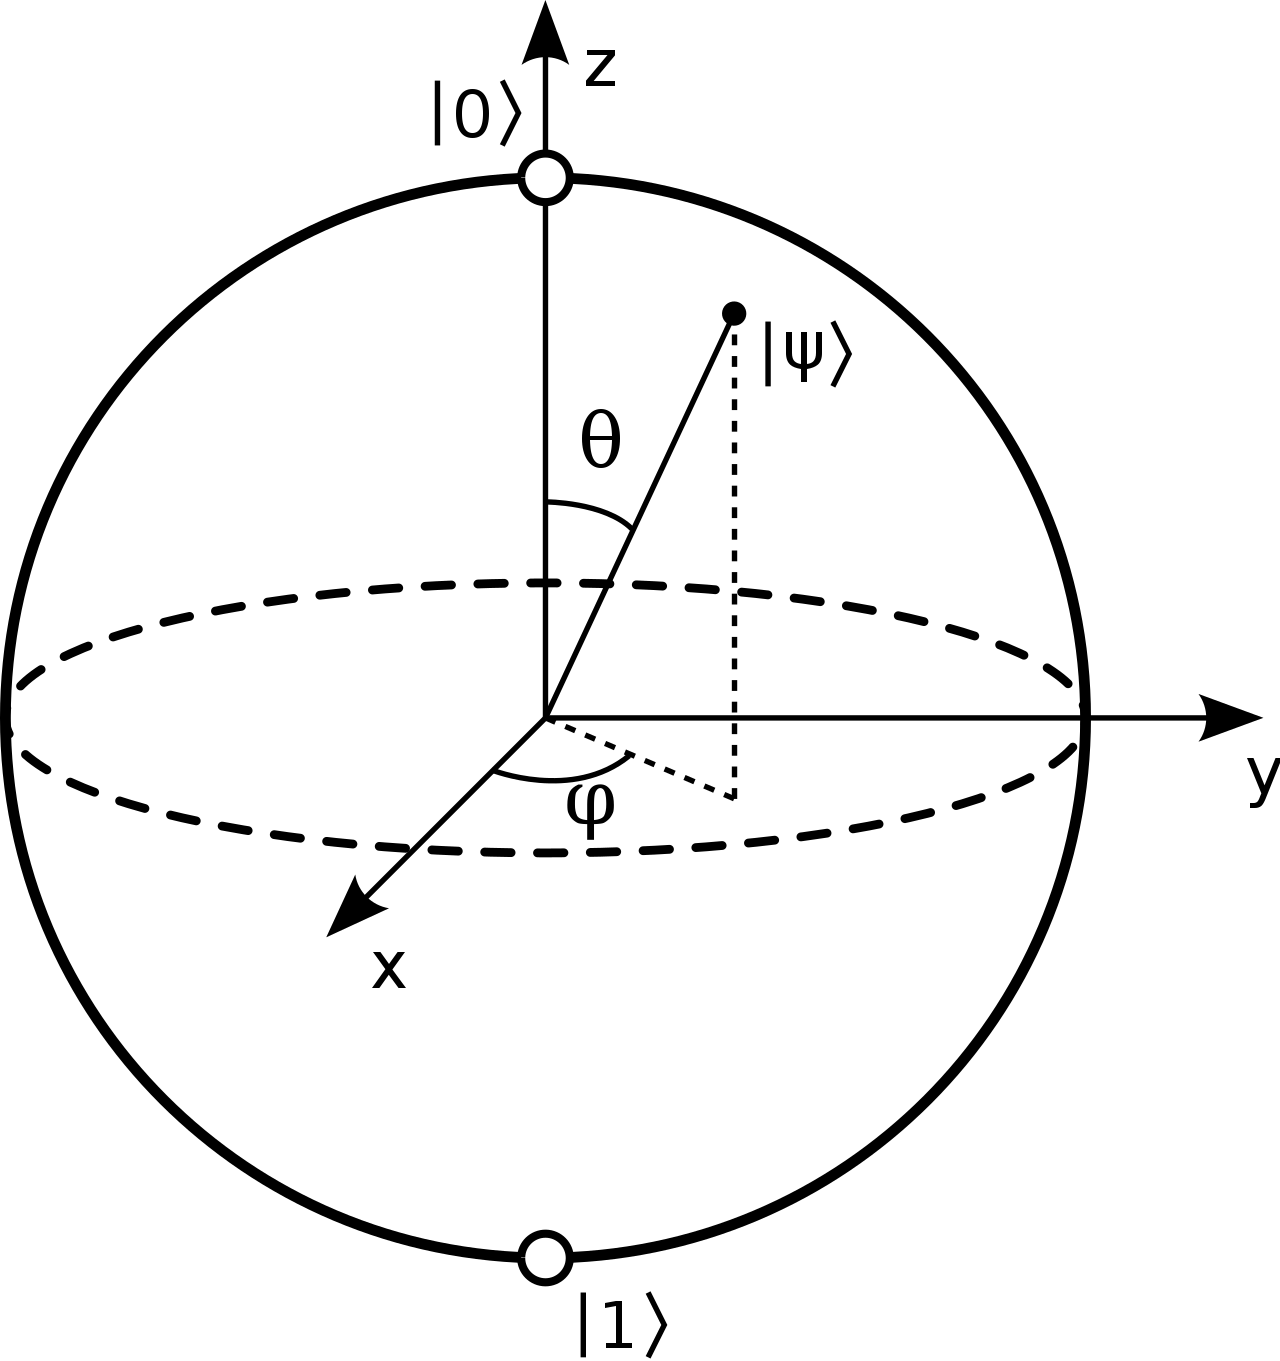
\includegraphics[width=2.5cm]{Bloch_sphere.svg.png}


	\begin{block}{\bf A few reasons ..}
		\begin{itemize}
		\item Some evidence that quantum can solve classically intractable problems
  		\item Nature is inherently quantum
		\begin{itemize}
  		\item Physicists and chemists need to solve hard simulation problems
  		\item Many problems physicists deal with are \QMA-complete (``Quantum \NP'')
		\end{itemize}
		\item Classical hardware is reaching its limitations
		\begin{itemize}
  		\item Quantum effects, like tunneling, put a spoke in the wheel
%  		\item Philosophically interesting
		\end{itemize}
		\end{itemize}
	\end{block}

\end{frame}


\begin{frame}{Why NOT Quantum Computing?}
\begin{refsection}

\vfill

\begin{alertblock}{What if the (error-corrected) quantum computer never materializes?}
		\begin{itemize}
		\item it turns out that \BQP{} = \P, or
		\item the device is too hard to build
		\end{itemize}
\end{alertblock}

\centering


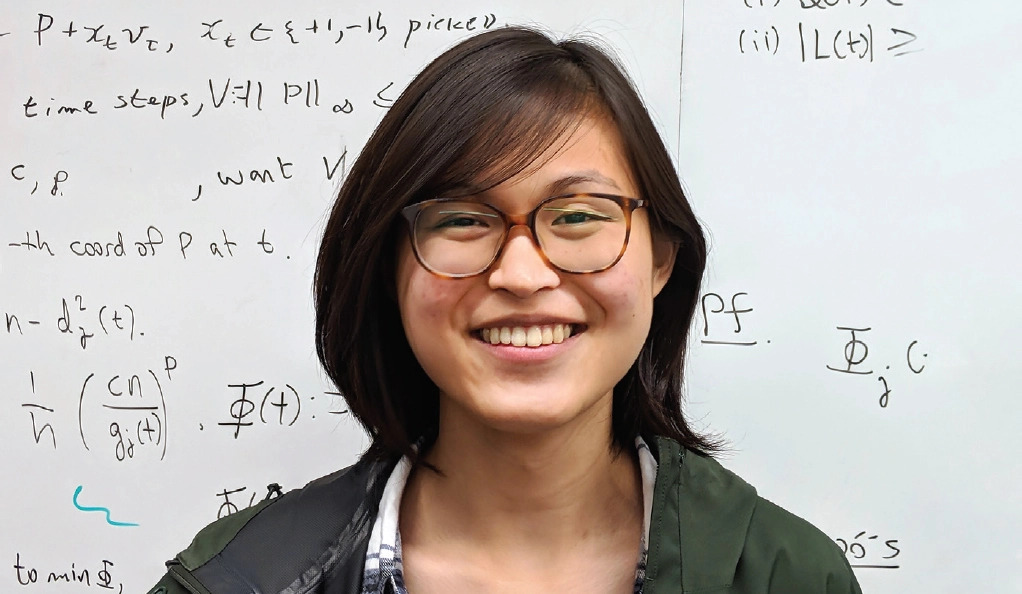
\includegraphics[width=4cm]{tang.jpeg}

 Ewin Tang~\cite{tang2019quantum}

\onslide<2->{
\alert{Regardless of whether a quantum computer ever gets build, we are improving our understanding of quantum-hard problems.}
}

%\vspace{-.5em}

\vfill
\printbibliography[section=\therefsection]

\end{refsection}
\end{frame}




\begin{frame}{On the Road to Quantum Supremacy}


\[
\scalebox{.8}{
\Qcircuit @C=1.em @R=.7em {
\lstick{\ket{0}} & & \gate{H} & \ctrl{1} 						&\qw	& \qw      & \qw  \\
\lstick{\ket{0}} & & \qw      & \gate{X} 						&\qw 	& \ctrl{1} & \qw  \\
\lstick{\ket{0}} &  & \qw      & \push{\rule{1.5em}{.4pt}}\qw 	& \qw 	& \gate{X} & \qw  
}}
\]

~\\

	\begin{block}{\bf How can we contribute?}
		\begin{itemize}
		\item Build an (error-corrected) quantum computer
		\item Come up with a new quantum algorithm that (conditionally) shows that $\BQP \neq P$
		\item {Invent the tools to use current and future quantum computers}
\pause
		\begin{itemize}
		\item \alert{Comparing data structures for representing quantum information}
		\item \alert{Quantum circuit compilation}
		\item \alert{Simulation and analysis of physical systems}
		\item \dots
		\end{itemize}
		\end{itemize}
	\end{block}

\end{frame}

\begin{refsection}
\begin{frame}{Quantum Circuit Compilation}


	\begin{block}{\bf Compilation is essential}
		\begin{itemize}
		\item Efficiently utilize early frugile quantum computers
%		\item ....
		\item Error correction requires hybrid solutions with fast classical components
		\end{itemize}
	\end{block}

\pause
\vspace{-.5em}

	\begin{block}{\bf Compilation entails...}
		\begin{itemize}
		\item {Quantum circuit simulation}~\cite{burgholzer2020advanced,viamontes2003improving,vinkhuijzen2021limdd}
		\item Quantum circuit optimization (topology, gate type minimization, ...)~\cite{shaik2023optimal}
%		\item Quantum circuit verification~\cite{}
		\item Quantum circuit equivalence checking~\cite{thanos2023fast,peham2022equivalence}
		\item Quantum circuit synthesis~\cite{brand2023quantum,}
		\end{itemize}
	\end{block}

\vspace{-.8em}

\printbibliography[section=\therefsection]

\pause
\centering
\alert{(We can use the power of formal methods \& automated reasoning tools)}


\end{frame}
\end{refsection}





\begin{frame}{Quantum Circuit Simulation}

\vfill

~~~~~~~~~~~~~~
\Qcircuit @C=2.3em @R=0.7em {
& \ket{0} & & \gate{H} & \ctrl{1} & \qw      & \qw  \\
& \ket{0} & & \qw      & \gate{X} & \ctrl{1} & \qw \\
& \ket{0} & & \qw      & \push{\rule{1.5em}{.4pt}}\qw & \gate{X} & \meter\\
&	  & & \dstick{U_1} & \dstick{U_2} & \dstick{U_3}  	 & \dstick{U_4}
\gategroup{1}{4}{3}{4}{.7em}{--}
\gategroup{1}{5}{3}{5}{.7em}{--}
\gategroup{1}{6}{3}{6}{.7em}{--}
\gategroup{1}{7}{3}{7}{.7em}{--}
}

\vfill

\vspace{1em}

\pause
\begin{exampleblock}{State-based simulation}
\centering
\scalebox{1.5}{
$ \ket{\phi_1} ~~=~~ U_1 \cdot \ket{\phi_0} $
}

\scalebox{1.5}{
$ \ket{\phi_2} ~~=~~ U_2 \cdot \ket{\phi_1} $
}

\scalebox{1.5}{
$ \ket{\phi_3} ~~=~~ U_3 \cdot \ket{\phi_2} $
}

\scalebox{1.5}{
$ \ket{\phi_4} ~~=~~ \hspace{-.07cm}\underbrace{U_4}_{\mathclap{\text{simple matrices}}}  \hspace{-.1cm} \cdot \ket{\phi_3} $
}
\end{exampleblock}

\pause

\begin{block}{Strong vs weak simulation}
	\begin{itemize}
		\item \textbf{Strong}: compute probability $\braket{b | \phi_3}$ of the measure outcome  for any $b\in \set{0,1}^n$
		\item \textbf{Weak}: sample the probability distribution $b\in \set{0,1}^n \to \braket{b | \phi_3}$

			\alert{(This is what a quantum computer does.)}
	\end{itemize}
\end{block}


\vfill
	
\end{frame}




\begin{refsection}
\begin{frame}{Verification: Circuit Equivalence Checking}

\vfill

\centering


\begin{columns}
\begin{column}{.05\textwidth}
\end{column}
\begin{column}{.4\textwidth}
\scalebox{1}{
\Qcircuit @C=1.em @R=.7em {
& & \gate{H} & \ctrl{1} 						&\qw	& \qw      & \qw  \\
& & \qw      & \gate{X} 						&\qw 	& \ctrl{1} & \qw  \\
&  & \qw      & \push{\rule{1.5em}{.4pt}}\qw 	& \qw 	& \gate{X} & \qw  
}}
\end{column}
\begin{column}{.08\textwidth}
\hspace{-.em}
\scalebox{2}{$\stackrel?\approx$}
\end{column}
\begin{column}{.4\textwidth}
\scalebox{1}{
\Qcircuit @C=1em @R=.7em {
& & \qw		  &  \gate{X}  						& \gate{H} 	& \qw      & \qw  \\
& & \gate{H}  &  \ctrl{-1}\qwx[0] 				& \gate{H} 	& \ctrl{1} & \qw \\
&  & \qw      & \push{\rule{1.5em}{.4pt}}\qw  	&\qw  		&   \gate{X}&\qw  
}}
\end{column}
\begin{column}{.05\textwidth}
\end{column}
\end{columns}

\vspace{.5cm}


\pause


We can reduce this problem to \alert{strong} simulation \cite{thanos2023fast}.

(A reduction to weak simulation would imply ``Quantum \P'' = ``Quantum \NP'')


\vfill

\printbibliography[section=\therefsection]
\end{frame}
\end{refsection}





\begin{frame}{Representing Quantum Information}
%	\framesubtitle{The proof uses \textit{reductio ad absurdum}.}



\begin{columns}%[onlywidth,T]
	\begin{column}{1\textwidth}
	\centering
\[
\def\arraystretch{1.15}
\underbrace{\scalebox{2}{$\ket{\phi}$}}_{n \text{ qubit state}}
~~~~~=~
\left.
\begin{bmatrix*}[c]
    \frac{i+1}{\sqrt 6} \\ 0 \\ 0 \\ 0\\ \vdots \\0\\ \frac1{\sqrt 3} \\ 0 \\\frac1{\sqrt 3} 
\end{bmatrix*}
~~\right \}\text{$2^n$-sized vector}
\]  
	\end{column}
\end{columns}

\begin{alertblock}{The Problem}
	\begin{itemize}
		\item A quantum state on $n$ qubits has $2^n$ amplitudes (complex numbers)
	\end{itemize}
\end{alertblock}



\end{frame}





\begin{frame}{This Talk}
	

\begin{block}{Study different exact representations of quantum states}
	\begin{itemize}
		\item \alert{(Generalized) Stabilizer Formalism}
		\item \alert{Decision Diagrams (DDs)}
	\begin{itemize}
		\item We introduce \alert{\limdd} to unify strengths of stabilizer formalism and DDs.
	\end{itemize}
		\item Tensor Networks (Matrix Product State in specific)
		\item Restrict Boltzmann Machine (RBM; a single layer neural network)
	\end{itemize}
	\vspace{-.5em}
\end{block}

\pause
\vspace{-.5em}

\begin{block}{Compare different representations analytically}
\vspace{-.5em}
	\begin{itemize}
		\item \textbf{Succinctness}: Families of quantum states showing exponential separations
		\item \textbf{Tractability}: Is manipulation of the representation (e.g., applying a gate) efficient
	\end{itemize}
	\vspace{-.5em}
\end{block}

\pause


\begin{columns}
\begin{column}{.45\textwidth}	
\centering
~~~~~~~~\begin{tikzpicture}\footnotesize
  \tikzset{venn circle/.style={circle,minimum width=2cm,fill=####1,opacity=0.4}}
  \node [venn circle=white,minimum width=4cm,draw] (A) at (0,0.3) {};
  \node  at (0,1.95) 			{State space};

  \node [venn circle = Red!40!white, ellipse,minimum height=2.2cm, minimum width=3.6cm] (L) at (0,0.6) {};
  \node  at (0,1.5) 		{poly-\alert{\limdd}};
  
  \node [venn circle = blue!70!white,text width=1.3cm,align=center,rotate=79,ellipse,minimum height=1.8cm, minimum width=2.5cm] (B) at (-.6,-.2) {};
  \node[text width=1.3cm,align=center]  at (-.7,-1.) {poly-MPS};


  \node [venn circle = green!70!white,text width=1.3cm,align=center,rotate=119,ellipse,minimum height=1.8cm, minimum width=2.5cm] (B) at (.6,-.2) {};
  \node[text width=1.3cm,align=center]  at (.9,-1.) {poly-RBM};



  \node [venn circle = Blue!100!white,text width=1cm,align=center, minimum width=1.cm] (B) at (-.5,.3) 	{\textcolor{white}{poly-QMDD}};						

  \node [venn circle = OliveGreen!100!white,text width=1cm,align=center, minimum width=1.cm] (C) at (.5,.2) {\textcolor{white}{Stabilizer states}};

\end{tikzpicture}
	\end{column}
	\begin{column}{.65\textwidth}
\setlength{\tabcolsep}{2pt}
\def\arraystretch{1.1}
\footnotesize
\begin{tabular}{|l@{\hspace{10pt}}|| *{5}{c|}| *{20}{c|}}
%\footnotesize
\hline
 & \multicolumn{5}{c||}{Queries} & \multicolumn{7}{c|}{Manipulation operations} \\
	& \rot{\samp} & \rot{\pro} & \rot{\eq}  & \rot{\inprod} & \multicolumn{1}{R{90}{0em}||}{\fid}
	& \rot{\addi} & \rot\had & \rot{\xyz} & \rot\cz & \rot{\swap} & \rot{\loc} & \rot{\T-gate} \\
\hline
Vector& \Yar & \Yes & \Yes & \Yes & \Yes & \Yes & \Yes & \Yes & \Yes & \Yes & \Yes & \Yes \\
\hline
%		| Sampl	| Prob 	| Eq	|Inprod	| Fid
ADD   	& \Yar	& \Yes	& \Yes	& \Yes & \Yes
%		| Add	| H		| XYZ	| CX	| Swap	| Local	| T
		& \Yes	& \Yes 	& \Yes	& \Yes	& \Yes	& \Yes	& \Yes \\
\hline
QMDD
		& \Yar	& \Yes	& \Yes	& \Yes & \Yes
		& \No	& \No 	& \Yes	& \Yes	& \No	& \No	& \Yes \\
\hline 
%QMDD  & \Yes & \Yes & \Yes & \No & \Yes & \No & ?? & ??  & ?? & \No & ?? & ??   \\
%\hline    
\alert{\limdd} 	& \Yar	& \Yes	& \Yes	& \Cond & \Cond
		& \No	& \No	& \Yes	& \Yes	& \No	& \No	& \Yes  \\
\hline 
%TN    & \Cond? & \Cond? & \Cond? & \Cond? & ?? & \Yes? & \Yes? & \Yes? & \Yes? & \Yes? & \Yes? \\ \hline
MPS   & \Yar & \Yes & \Yes & \Yes & \Yes & \Yes 
	  & \Yes & \Yes & \Yes & \Yes & \Yes & \Yes  \\
\hline 
RBM   & \Yar    & ? & ? & \Cond & \Cond & ? & ? & \Yes & \Yes & \Yes & ? & \Yes \\
\hline 
%\multicolumn{13}{c}{Low priority} \\
%\hline 
%ZX    & ?? & ?? & ?? & ?? & ?? & ?? & ?? & ?? & ?? & ?? & ?? & ?? \\
%\hline 
%SLDD$_+$  & \Yes? & \Yes? & \Yes? & \Yes? & \Yes? & \No! & \No? & \Yes? & \No! & \No! & \No? & \Yes! \\
%\hline 
\end{tabular}	
\end{column}
\end{columns}

\end{frame}

















\begin{frame}
\vfill


\Large

\begin{quote}
``Quantum computing becomes easy once you take the physics out of it''
\end{quote}
\hfill
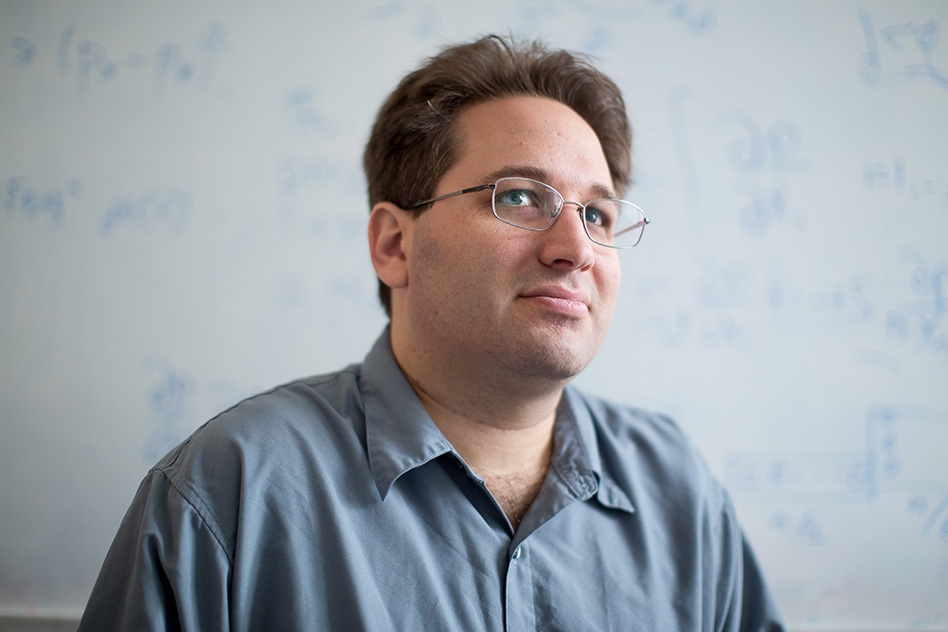
\includegraphics[width=5cm]{scott-aaronson.jpeg}

\hfill Scott Aaronson

%\hfill \url{https://scottaaronson.blog}
\end{frame}





\begin{frame}{Quantum States}
%	\framesubtitle{The proof uses \textit{reductio ad absurdum}.}



\begin{columns}%[onlywidth,T]
	\begin{column}{.4\textwidth}
\[
\def\arraystretch{1.15}
\underbrace{\scalebox{2}{$\ket{\phi}$}}_{n \text{ qubit state}}
~~~~~=~
\left.
\begin{bmatrix*}[c]
    \frac{i+1}{\sqrt 6} \\ 0 \\ 0 \\ 0\\ \vdots \\0\\ \frac1{\sqrt 3} \\ 0 \\\frac1{\sqrt 3} 
\end{bmatrix*}
~~\right \}\text{$2^n$-sized vector}
\]  
	\end{column}
%\pause
	\begin{column}{.6\textwidth}
\vspace{3mm}\[
\def\arraystretch{1.2}
\scalebox{1.}{$\ket{00\dots01}$}
~=~
\begin{bmatrix*}[c]
    0 \\ 1 \\ 0 \\ 0\\ \vdots \\0\\ 0  \\ 0 \\ 0 
\end{bmatrix*}
\begin{matrix*}[c]
	{\text{$\leftarrow$ index \scriptsize 00\dots00 }} \\ 
	{\text{$\leftarrow$ index \scriptsize 00\dots01 }} \\ \\ \\ \\ \\ \\ \\  
	{\text{$\leftarrow$ index \scriptsize 11\dots10 }} \\  
	{\text{$\leftarrow$ index \scriptsize 11\dots11 }} \\ 
\end{matrix*}
\]  	
	\end{column}
\end{columns}
\pause
\begin{columns}%[onlywidth,T]
	\begin{column}{1\textwidth}
\[
\def\arraystretch{.9}
\scalebox{2}{$\ket{\phi}^\dagger$}
~~=~~
\scalebox{2}{$\bra{\phi}$}
~~=~~
\underbrace{
\begin{bmatrix*}[c]
    \frac{\alert -i+1}{\sqrt 6} ,& 0 ,& 0 ,& 0,& \dots ,&0,&  \frac1{\sqrt 3} ,& 0 ,& 0 ,& \frac1{\sqrt 3} 
\end{bmatrix*}
}_{\text{$2^n$-sized vector (\alert{conjugated} and transposed)}}
\]  
	\end{column}
\end{columns}

\pause

  	\begin{block}{Normalization}
		For $\ket{\phi} =  \begin{bmatrix}\alpha_1, \alpha_2, \dots, \alpha_{n-1}, \alpha_n\end{bmatrix}^T$, we have that $\sum |\alpha_i|^2 = 1$.
		
		~\\
		Or alternatively: $\braket{\phi|\phi} = \bra{\phi}\cdot \ket{\phi} = 1$.
  	\end{block}


%  	\begin{block}{Alternative interpretation as pseudo-Boolean function}
%%  		\begin{itemize}
%%  			\item 
%  			A pseudo-Boolean function $f_\phi \colon \set{0,1}^n \to \complex$ such that $f(b) = \braket{b|\phi} = \bra{b}\cdot \ket{\phi}$.
%%  			\\
%%  			~\\
%%  			Here $\bra{b}$ for $b \in \set{0,1}^n$ is a (conjugated) computational basis state, e.g.: $\bra{01} = \begin{bmatrix}0, 0, 0, 0\end{bmatrix}$.
%%  		\end{itemize}
%  	\end{block}


\end{frame}







\begin{frame}{Quantum Gates and Circuits}

\begin{block}{Definition}
	An $n$-qubit quantum gate is an $2^n \times 2^n$ complex matrix preserving norm (unitary).
\end{block}



\begin{exampleblock}<+->{The Bell state}



\begin{align*}&\phantom{Zf}
\Qcircuit @C=1em @R=1.3em {
&   	 & &  &  
\rstick{	
\onslide<6->{
\def\arraystretch{1.1}
    \frac1{\sqrt 2}\cdot
    \begin{bmatrix*}[c]
    1\\ 0 \\ 0\\1\\
    \end{bmatrix*}
    \begin{matrix*}[c]
   \\\\\\ \\
    \end{matrix*}
}
}
 & & \\
&   	 & &  &  &&   \\
\lstick{\ket{0}}	& \qw	& \gate{H} & \qw& \qw & \ctrl{1}  
& \qw \ar@{--}[]+<.5em,1em>;[d]+<.5em,-1em> & \qw &	 \meter 
 & \rstick{ 
 		%hide meter:
 		\hspace{-1cm}\only<1-7>{\raisebox{-.5em}{\crule[LEIdarkgreen!10]{2cm}{.5cm}}}
	 	\onslide<9>{
	 				~~~~~~~~~
	 				\alert{
	 				\text{collapses to }
	 				\begin{bmatrix*}[r]
				    1\\ 0 \\ 0\\0 \\
			    	\end{bmatrix*}
   						\begin{matrix*}[c]
    						=\ket{00}\\\\\\ \\
    					\end{matrix*}
			    	\alert{or}
			    	\begin{bmatrix*}[r]
				    0\\ 0 \\ 0\\1 \\
			    	\end{bmatrix*}
   						\begin{matrix*}[c]
    						\\\\\\=\ket{11} \\
    					\end{matrix*}
			    	}
 				}
 			} 
 			\\
%\lstick{
%\def\arraystretch{1.1}
%    \raisebox{5em}{
%    $
%    \mat{1\\0}
%    \otimes 
%    \mat{1\\0} =
%    \begin{bmatrix*}[c]
%    1\\ 0 \\ 0\\0\\
%    \end{bmatrix*}$
%    }
%} 		
\lstick{\ket{0}}			
	& \qw	& \qw& \qw& \qw & \targ & \qw & \qw &\qw &
 \\
&   	 & &  &  && \\
}
&
\end{align*}


\pause

  $
   \ket{0} \otimes \ket{0} = \ket{00}=
    \smat{1\\0}
    \otimes 
    \smat{1\\0} =
    \begin{bsmallmatrix*}[c]
    1\\ 0 \\ 0\\0\\
    \end{bsmallmatrix*}
    $

\vspace{1em}

\pause

$ 
%	\underbrace{
%		\begin{bsmallmatrix*}[r]
%		1& 0& 0& 0 \\
%    	0& 1& 0& 0 \\
%	    0& 0& 0& 1 \\
%	    0& 0& 1& 0 \\
%    	\end{bsmallmatrix*}
%    }_{CNOT}
%    \cdot
%    H\otimes I
%    \cdot
%    \begin{bsmallmatrix*}[c]
%    1\\ 0 \\ 0\\0\\
%    \end{bsmallmatrix*}
%    ~=
%\pause 
%	\alert{
%	}
%	\cdot
	 \underbrace{
		\begin{bsmallmatrix*}[r]
		1& 0& 0& 0 \\
    	0& 1& 0& 0 \\
	    0& 0& 0& 1 \\
	    0& 0& 1& 0 \\
    	\end{bsmallmatrix*}
    }_{CNOT}
	\cdot
	\underbrace{
    	\frac1{\sqrt 2}\cdot
		\begin{bsmallmatrix*}[r]
		1& 0& 1& 0 \\
    	0& 1& 0& 1 \\
	    1& 0& -1& 0 \\
	    0& \phantom- 1& 0& -1 \\
    	\end{bsmallmatrix*}
    }_{H\otimes \id  }
    \cdot
    \underbrace{
    	\begin{bsmallmatrix*}[r]
    	1\\ 0 \\ 0 \\0  \\
	    \end{bsmallmatrix*}
    }_{
    	\begin{bsmallmatrix*}[r]
    	1\\0
    	\end{bsmallmatrix*}^{\otimes 2}
       }
 	=~
\pause
	\frac1{\sqrt 2}
	 \underbrace{
		\begin{bsmallmatrix*}[r]
		1& 0& 0& 0 \\
    	0& 1& 0& 0 \\
	    0& 0& 0& 1 \\
	    0& 0& 1& 0 \\
    	\end{bsmallmatrix*}
    }_{CNOT}
    \cdot
    	\begin{bsmallmatrix*}[r]
    	1\\ 0 \\ 1 \\0  \\
		\end{bsmallmatrix*}
= 
	\frac1{\sqrt 2}\cdot
    \begin{bsmallmatrix*}[c]
    1\\ 0 \\ 0\\1\\
    \end{bsmallmatrix*}
%    	\frac 1{\sqrt 2}\cdot
%%    \underbrace{
%    	\begin{bsmallmatrix*}[r]
%	    1\\ 0 \\ 0\\1 \\
%    	\end{bsmallmatrix*}
%    }_{
%	    \mathclap{
%    	\begin{bsmallmatrix*}[r]
%    	1\\0
%    	\end{bsmallmatrix*}^{\otimes 2}
%    	\alert{+}
%    	\begin{bsmallmatrix*}[r]
%    	0\\1
%    	\end{bsmallmatrix*}^{\otimes 2}
%    	}
%    }
$
\end{exampleblock}

\pause[10] %for revealing the \meter

\centering
\alert{Gate matrices are large but often very structured.}


\end{frame}





\section{Quantum Information}


\begin{frame}
\begin{refsection}
	
\vfill

\vspace{-.5cm}\textbf{\Large Quantum Computing with \#SAT}~\cite{mei2024simulating,mei2024eq}\vspace{-.5cm}

\vfill

\printbibliography[section=\therefsection]
\end{refsection}

\end{frame}





\begin{frame}{Weighted Model Counting (\#SAT)}


Model counting (\#SAT) is the counting version ($\#\P$) of satisfiability (SAT).

\pause

~\\
~\\

\begin{definition}[Weighted Model Counting]
Given a 
	\alert{CNF formula} $F(V) \colon \mathbb B^n \to \mathbb B$ and a 
	\alert{weight function} $W\colon \set{ \bar v, v \mid v\in V} \to \mathbb{C}$, 
%For a propositional formula $F$ over variables in $V$ and weight function $W$, 
we define \concept{weighted model counting} as follows.
\[
MC_W(F) \defn   \sum_{\alpha \in  \bool^V} F(\alpha)\cdot W(\alpha)\text{, where }  W(\alpha) = \prod_{v\in V} W(\alpha(v)).
\]
\end{definition}	

\pause

\begin{example}{}
  Given the formula $F = (a \vee b) \land  c$ over $V=\{a,b, v\}$ with weights $W(a) = \frac13, W(\bar a) = \frac23$ ($a, b$ always have weight 1), the model count is:
  

\hfill 
  \begin{tabular}{|l|l|}
  \hline
  	$\bar a  b  c$ & $\nicefrac 23$ \\
  	 $a \bar b  c$ & $\nicefrac 13$ \\
  	$a b  c$ & $\nicefrac 13$\\
  \hline
  \end{tabular}  
  \hfill 
  $\nicefrac 23 + \nicefrac 13 + \nicefrac 13= \nicefrac 43$
\hfill ~

\end{example}


\end{frame}






\begin{frame}{Encoding in weighted model counting}

\vspace{-1em}
  \[
    \begin{array}{c}  
      \Qcircuit @C=1em @R=.7em {
        \lstick{\ket{0}_{\alert x}} & \qw\ar@{.}[]+<0em,1em>;[d]+<0em,-0.5em> & \gate{H ~\alert{(h)}} &\qw\ar@{.}[]+<0em,1em>;[d]+<0em,-0.5em> & \ctrl{1} & \qw\ar@{.}[]+<0em,1em>;[d]+<0em,-0.5em> &\qw & \qw\ar@{.}[]+<0em,1em>;[d]+<0em,-0.5em> &\qw & \rstick{\action<8->{\bra{0}}}  \\
        \lstick{\ket{0}_{\alert y}} & \qw & \qw & \qw & \targ & \qw &\gate{T~\alert{(t)}}&\qw &\qw& \rstick{\action<8->{\bra{0}}} \\
        & \ket{\varphi_0} & & \ket{\varphi_1} & & \ket{\varphi_2} & & \ket{\varphi_3} & &
      }
    \end{array}		
  \]

  % \begin{quantikz}
  %   \slice{\varphi_0 = \ket{0}} & \gate{H}\slice{\ket{\varphi_1}} & \ctrl{1}\slice{\ket{\varphi_2}} & \\
  %                               &                                 & \targ{}                          & \gate{T}\slice{\ket{\varphi_3}}\\
  % \end{quantikz}
 
\centering
\alert{where $x$, $y$, $h$ and $t$ are Boolean variables. We copy $x,y$ for every time step:}
 
\pause

\vspace{-1em}

\hspace{-3em}
\begin{minipage}{\textwidth}
  \begin{align*}
    \ket{\varphi_0} &&&= \ket{00} && \equiv \bar x_0 \bar y_0\\
     \action<3->{\ket{\varphi_1} &= (H \otimes I) \ket{\varphi_0} &&= \tfrac{1}{\sqrt{2}}\ket{00}+\tfrac{1}{\sqrt{2}}\ket{10} &&  
    		%F_{H_a}(\vec{x}_0, \vec{x}_1) = 
    		\equiv {\color{gray}\bar x_0 \bar y_0} ~~\land ~~ \bar y_1 h 
    							 \text{ ~~\alert{$W(h) = \nicefrac{1}{\sqrt{2}}$}} \\}
     \action<4->{\ket{\varphi_2} &= CX\ket{\varphi_1} 
    				&&= \tfrac{1}{\sqrt{2}}\ket{00}+\tfrac{1}{\sqrt{2}}\ket{11} &&
    						%F_{CX}(\vec{x}_1, \vec{x}_2) 
    						\equiv \dots  {\color{gray} h}  \dots  ~~\land ~~ (\bar x_2 \bar y_2 ~~\vee~~  x_2 y_2)\\}
     \action<5->{\ket{\varphi_3} &= (I\otimes T)\ket{\varphi_2} &&= \tfrac{1}{\sqrt{2}}\ket{00}+\tfrac{e^{i\nicefrac\pi4}}{\sqrt{2}}\ket{11} && % F_{T_1}(\vec{x}^2, \vec{x}^3) 
    			\equiv \dots  {\color{gray} h}  \dots ~~\land~~ (\bar x_3 \bar y_3 \bar t ~~\vee~~ x_3 y_3 t)}
  \end{align*}
 \pause[5]
%  $ = -\frac{1}{\sqrt{2}}$, $W(u)=e^{i\pi/4}$ and $W(\bar u)=1$.
\hfill\alert{where  $W(\bar t)=1$ and $W(t)=e^{i\nicefrac\pi4}$}
\end{minipage}

\pause

%  \keymessage{The encoding for all three gates would be
\begin{block}{Gate Encoding}
    \begin{itemize}
      \item $F_{H}(x, x',h) ~~~~~~~~\defn  \bar h \Leftrightarrow x  x' $ \hfill  
				\alert{$W(h) = \nicefrac{1}{\sqrt{2}},  W(\bar h) = -\nicefrac{1}{\sqrt{2}}$}
      \item $F_{CX}(x,y,x',y') ~~\defn   x' \Leftrightarrow  x ~~\land~~ (y'\oplus y) \Leftrightarrow  x $
      \item $F_{T}(x,x',t) ~~~~~~~~\defn x' \Leftrightarrow  x ~~\land~~  t \Leftrightarrow  x$
    \end{itemize}
\end{block}

\pause

$\bar x_0 \bar y_0 ~~\land~~  F_H(x_0,x_1, h)\alert{\land y_1 \Leftrightarrow y_0} ~~\land~~  F_{CX}(x_1,y_1,x_2,y_2)  ~~\land~~ F_{T}(y_2,y_3,t)\alert{\land x_3 \Leftrightarrow x_2} \pause ~~\land~~ \bar x_3 \bar y_3$


%  }
\end{frame}



\begin{frame}{Constructive and destructive interference}

   \[
     \begin{array}{c}  
       \Qcircuit @C=1em @R=.7em {
         \lstick{\ket{0}_x} & \qw\ar@{.}[]+<0em,1em>;[d]+<0em,-0.5em> & \gate{H} &\qw\ar@{.}[]+<0em,1em>;[d]+<0em,-0.5em> & \gate{H} & \qw\ar@{.}[]+<0em,1em>;[d]+<0em,-0.5em> &\qw \\
         & \ket{\varphi_0} & & \ket{\varphi_1} & & \ket{\varphi_2} & &
       }
     \end{array}		
   \]

  \begin{align*}
  \ket{\phi_0} &= \ket 0\\
  \ket{\phi_1} &= \frac1{\sqrt 2}(\ket 0 + \ket 1)\\
  \ket{\phi_2} &= \frac1{\sqrt 2}(\frac1{\sqrt 2}(\ket 0 \underbrace{+ \ket 1}_{}) + \frac1{\sqrt 2}(\ket 0 \underbrace{- \ket 1}_{})) &= \ket 0
  \end{align*}


\pause




~\\

\centering
$\bar x_0  ~~\land~~  F_H(x_0,x_1, h) ~~\land~~ F_{H}(x_1,x_3,h')$

\pause


~\\
~\\
Satisfying assignments at each time step:
\[
\set{\bar x_0} \quad\quad\quad\quad  \set{~ \bar x_1 h,~~  x_1h ~} 
				\quad\quad\quad\quad  \set{~ {\color{gray}\bar x_1h }\, \bar x_2 h',~~  {\color{gray} x_1h}\, \bar x_2 h',~~ {\color{gray}\bar x_1 h}\,  x_2h',~~  {\color{gray} x_1 h}\,  x_2h'  ~} 
\]

\end{frame}




\begin{frame}{Encoding in weighted model counting}
Two major problems:
\begin{itemize}
  \item Generalization of measurement is hard: e.g. measuring individual qubits will result in adding amplitudes (instead of probabilities)
  \item To check equivalence of two circuits, one has to check \alert{exponential many basis states}.
 		\[
    % \arraystretch{1.3}
  \begin{matrix*}[c]
  \text{index }\overbrace{000\dots000}^{\mathclap{\text{\alert{computational basis state}}}}:\\\text{index }{000\dots001}:\\\text{index }{000\dots010}:\\\text{index }{000\dots011}:\\\vdots\vspace{1em}\\\\\text{index }\underbrace{111\dots111}_{\vspace{3em}}:\\
  \end{matrix*}
  \left.
  \begin{bmatrix*}[c]
   i \\0 \\ 0\\ 0 \\ \vdots \\ 0 \\ 0\\ 0  \\
  \end{bmatrix*}
  \right\}\text{ $2^n$}
\]
\item Modern weighted model counter does not support \alert{complex weights}.
\end{itemize}

\pause
\vspace{2em}
{\color{red}\textbf{Solution}: Move from computational basis to Pauli basis!}

\end{frame}












\begin{frame}{Pauli basis}
        \begin{itemize}
                \item Quantum states in vector form: $\ket{\phi} = \frac{1}{\sqrt{2}}(\ket{0} + \dot{\imath} \ket{1}) 
                = \frac{1}{\sqrt{2}} \begin{bmatrix}
                        1 \\
                        \dot{\imath}
                \end{bmatrix}$
                \item Quantum states in density operator form: 
                $\dyad{\phi} = \frac{1}{2} \begin{bmatrix} 1 \\ \dot{\imath} \end{bmatrix}\cdot [1, -\dot{\imath}] = 
                \frac{1}{2}
                \begin{bmatrix}
                        1 & -\dot{\imath} \\
                        \dot{\imath} & 1
                \end{bmatrix}
                $.
        \end{itemize}

        \pause
        \[
   I\, \equiv
    \begin{bmatrix}
      1 & 0 \\
      0 & 1
    \end{bmatrix},
    \quad
    Z \equiv
    \begin{bmatrix*}[r]
      1 & 0 \\
      0 & -1
    \end{bmatrix*},
    \quad
    X \equiv
    \begin{bmatrix*}[r]
      0 & 1 \\
      1 & 0
    \end{bmatrix*},
    \quad
     Y \equiv
    \begin{bmatrix*}[r]
      0 & -\dot{\imath} \\
      \dot{\imath} & 0
    \end{bmatrix*}
.
\]
\pause

\[
        \dyad{\phi} = \frac{1}{2}(Y+I)
\]
        Note the complex numbers in the density matrix, while the Pauli coefficients are real.

\pause
\begin{block}{In general}
    Any $n$-qubit density matrix $\rho = \dyad{\phi}$  can be decomposed into in the Pauli basis:
    \[
       \rho = \sum_i \alpha_i P_i
    \]
    where $P_i\in\{I,Z,X,Y\}^{\otimes n}$ is a Pauli string and $\alpha_i\in\mathbb{R}$.
%    This result can be generalized to multi-qubit case with tensor product.
\end{block}

\end{frame}



\begin{frame}{Encoding Gates in the Pauli Basis}
	

Gates act by conjugation on density matrices / Pauli strings, e.g.: $H Z H^\dagger = X$

\pause

  \setlength{\tabcolsep}{3pt} 
  \begin{tabular}{c|rr||c|cc||c|cc}
      \toprule
      \textbf{Gate} & \textbf{In} & \textbf{Out} & \textbf{Gate} & \textbf{In} & \textbf{Out} & \textbf{Gate} & \textbf{In} & \textbf{Out} \\
      \midrule
      & $X$ & $Z$ & \multirow{6}{*}{CZ} & $\phantom{-}I_c \otimes X_t$ & $\phantom{-}Z_c\otimes X_t$ && $X$& $\frac1{\sqrt2}(X+Y)$ \\
      $H$ & $Y$ & $-Y$ & & $\phantom{-}X_c \otimes I_t$ & $\phantom{-}X_c \otimes Z_t$ & $T$ & $Y$ & $\frac1{\sqrt2}(Y - X)$ \\
      & $Z$ & $X$ & & $\phantom{-}I_c \otimes Y_t$ & $\phantom{-}Z_c \otimes Y_t$   &&$Z$ & $Z$ \\
      \cline{1-3} \cline{7-9}
       & $X$ & $Y$ & & $\phantom{-}Y_c \otimes I_t$ & $\phantom{-}Y_c \otimes Z_t$  &&$X$& $X$  \\
      $S$ & $Y$ & $-X$ & & $\phantom{-}I_c \otimes Z_t$ & $\phantom{-}I_c \otimes Z_t$  &$R_X(\theta)$& $Y$& $\cos(\theta)Y + \sin(\theta) Z$ \\
      & $Z$ & $Z$ & & $\phantom{-}Z_c \otimes I_t$ & $\phantom{-}Z_c \otimes I_t$ && $Z$& $\cos(\theta)Z - \sin(\theta) Y$\\
      \bottomrule
  \end{tabular}

\pause
\hphantom{\cite{aaronson2008improved}}




For a qubit use Boolean variables $x,z$:\\
\[
\bar x \bar z \equiv I \quad\quad\quad  x \bar z \equiv X  \quad\quad\quad x  z \equiv Y \quad\quad\quad \bar x  z \equiv Z
\]


\pause

%  \keymessage{The encoding for all three gates would be
\begin{block}{Gate encoding}
    \begin{itemize}
      \item $F_{H}(x, z, x', z', s) \defn x' \Leftrightarrow z ~\land~ z' \Leftrightarrow x ~\land~ s \Leftrightarrow xz $ \hfill  $W(s) = -1$ / $W(\bar s) = 1$
      \item \dots %$F_{CX}(x,y,x',y') ~~\defn   x' \Longleftrightarrow  x ~~\land~~ (y'\oplus y) \Longleftrightarrow  x $
\pause
      \item $F_{T}(x, z, x', z', t) \defn x' \Leftrightarrow  x ~\land~  (\bar x \Rightarrow (z' \Leftrightarrow  z)) ~\land~  t \Leftrightarrow  x \dots$ \\
		\hfill  $W(t) = \tfrac1{\sqrt 2}$ / $W(\bar t) = 1$
    \end{itemize}
\end{block}


  
	
\end{frame}



\begin{refframe}{\#SAT-based Quantum Circuit Simulation}

Simulating Quantum Circuits by Weighted Model Counting (WMC) \cite{mei2024simulating}

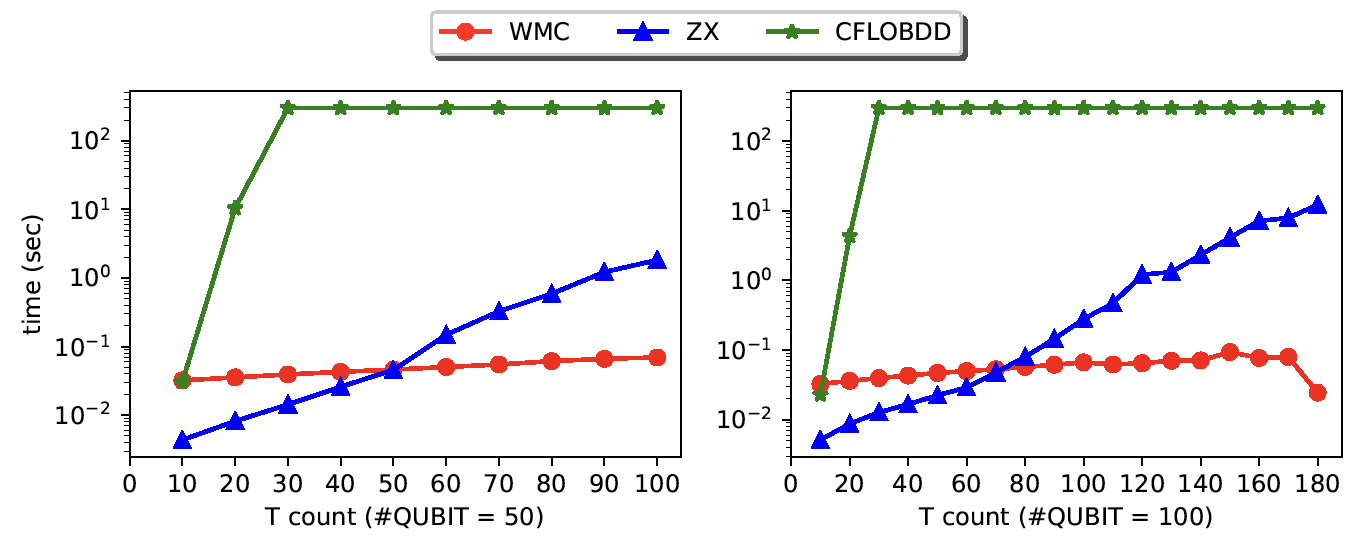
\includegraphics[height=4.5cm]{graphics/random-quokka}

Random circuits mimicking quantum chemistry applications from~\cite{kissinger_simulating_2022}.


\end{refframe}






\begin{refframe}{Encoding of equivalence checking}

\begin{definition}[Circuit Equivalence]
    Given two $n$-qubit circuits $U$ and $V$ where $n\in \mathbb{N}^+$,
    $U$ is equivalent to $V$, written $U\equiv V$, if there exists a complex number $c$ (the \concept{global phase}) such that for all input states $\ket{\psi}$, we have $U\ket{\psi} = cV\ket{\psi}$.
\end{definition}


\pause

    For an $n$-qubit quantum system, applying a single-qubit gate $P$ on the $j$-th qubit is 
 represented by 
 \begin{equation}
     P_j = I^{\otimes j -1}\otimes P \otimes I^{\otimes n- j},
     \label{eq:uj}\end{equation}

\pause

    \begin{theorem}[\cite{ours}]\label{thm:main-theorem}
        Let $U, V$ be two circuits on $n \in \mathbb{N}^{+}$ qubits.
        Then $U$ is equivalent to $V$ if and only if the following condition holds (for notation $P_j$ see \autoref{eq:uj}):\\
        For all $P \in \set{X_j, Z_j \mid j\in [n]}$, we have $U P_j U^{\dagger} = V P_j V^{\dagger}$.
    \end{theorem}

\end{refframe}


\begin{refframe}{Equivalence Checking Performance}

~
\hspace{-1.5cm}
	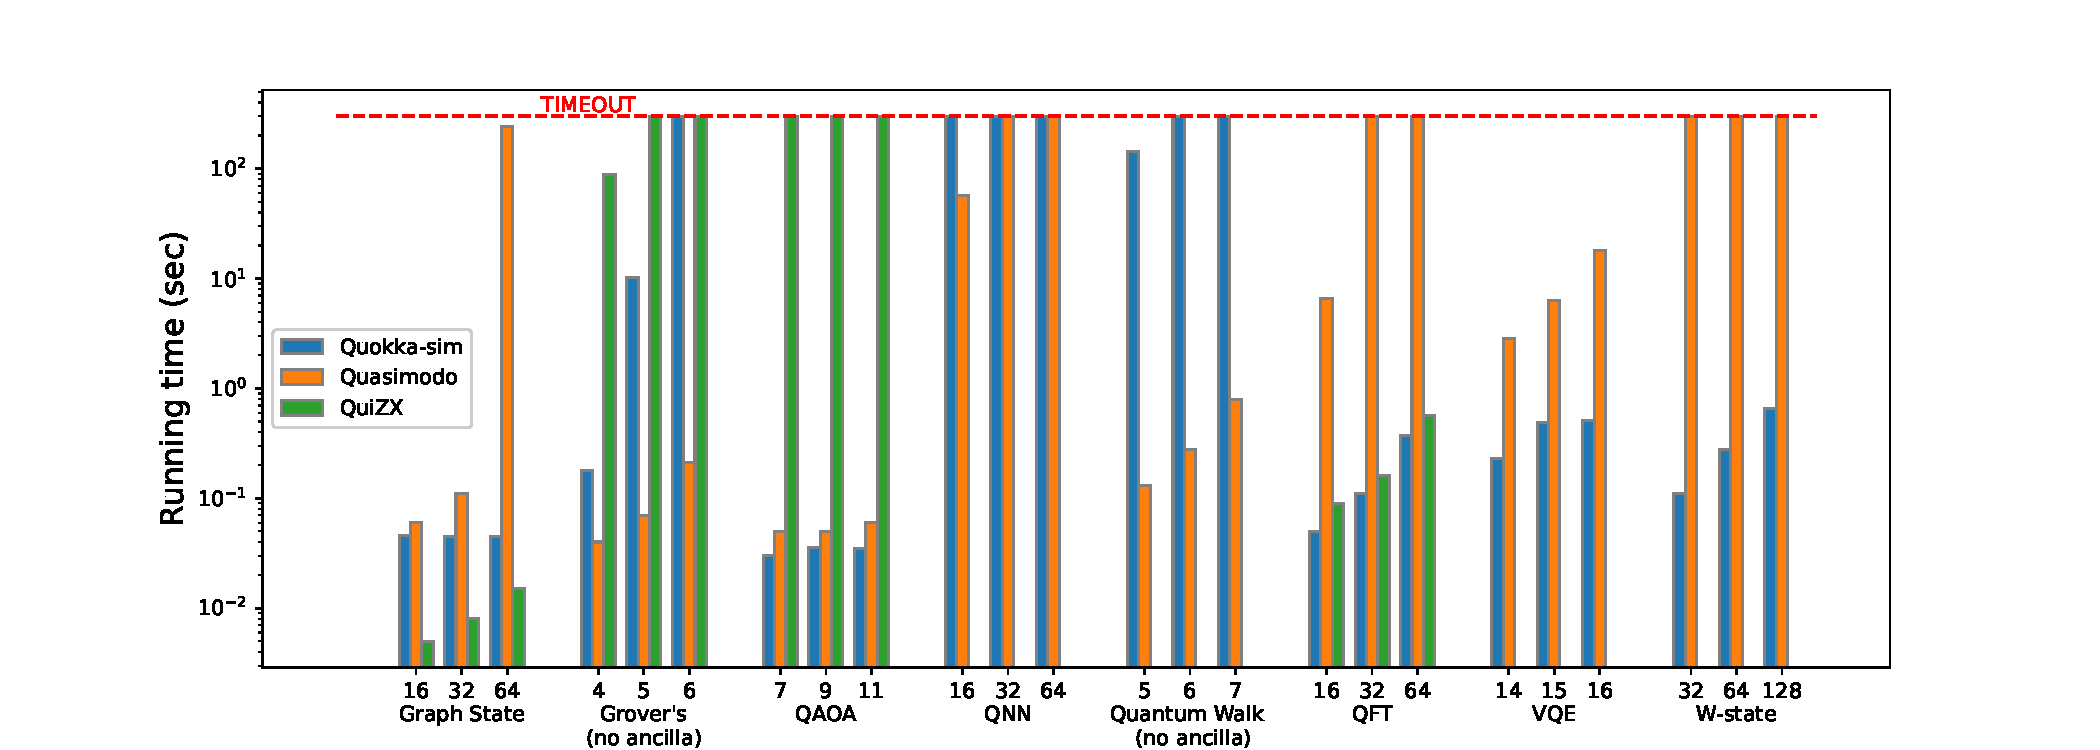
\includegraphics[width=14cm]{bar_sim}

\phantom{\cite{mei2024eq}}

\end{refframe}



\begin{refframe}{Quokka\#}

	\centering

\vspace{-4em}
	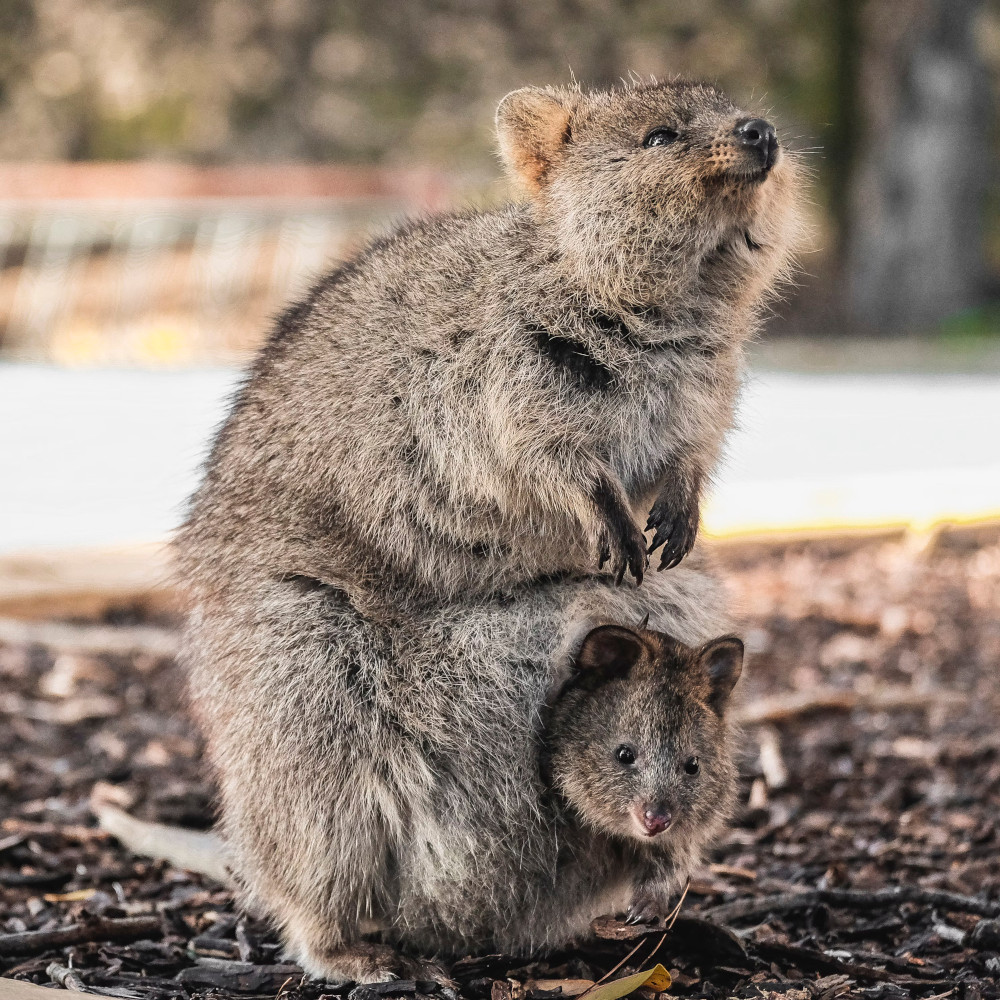
\includegraphics[width=4cm]{quokka}
	
	
\begin{alertblock}{The Quokka\# Tool}
	\begin{itemize}
		\item Linear-length \#SAT encoding of quantum circuits
		\item Simulation and equivalence checking
	\end{itemize}
	
	
\end{alertblock}

	
	\url{https://github.com/System-Verification-Lab/Quokka-Sharp}
	
	
\end{refframe}






\section{LIMDD}


\begin{frame}
\begin{refsection}

\vfill
	
	\centering
	\textbf{\Large Stabilizer Formalism, Decision Diagrams and \limdd~\cite{limdd}}
	
	
\vfill

\printbibliography[section=\therefsection]
\end{refsection}

\end{frame}




\begin{refframe}{Quantum State Representation with the
					\alert{Stabilizer Formalism}}


\begin{definition}[Stabilizer States~\cite{aaronson2008improved}]

\begin{itemize} 
	\item
A non-universal subset of all quantum states \alert{crucial for error correction, etc}: 

\begin{center}
\scalebox{.7}{
\begin{tikzpicture}\footnotesize
  \tikzset{venn circle/.style={circle,minimum width=2cm,fill=####1,opacity=0.4}}
  \node [venn circle=white,minimum width=2.5cm,draw] (A) at (0,0.3) {};
  \node  at (0,1.25) 			{State space};

%  \node [venn circle = Red!40!white, ellipse,minimum height=2.2cm, minimum width=3.6cm] (L) at (0,0.6) {};
%  \node  at (0,1.5) 		{\limdd};
  
%  \node [venn circle = blue!70!white,text width=1.3cm,align=center,rotate=79,ellipse,minimum height=1.8cm, minimum width=2.5cm] (B) at (-.6,-.2) {};
%  \node[text width=1.3cm,align=center]  at (-.9,-1.) {MPS};


%  \node [venn circle = green!70!white,text width=1.3cm,align=center,rotate=119,ellipse,minimum height=1.8cm, minimum width=2.5cm] (B) at (.6,-.2) {};
%  \node[text width=1.3cm,align=center]  at (.9,-1.) {RBM};



%  \node [venn circle = Blue!100!white,text width=1cm,align=center, minimum width=1.cm] (B) at (-.5,.3) 	{\textcolor{white}{QMDD}};						

  \node [venn circle = OliveGreen,text width=1cm,align=center, minimum width=1.cm,opacity=.5,text opacity=1] (C) at (.5,.2) {\textcolor{white}{Stabilizer states}};
\end{tikzpicture}
}		
\end{center}

\pause

\item A stabilizer state $\ket{\phi}$ is uniquely defined by   
			$n$-qubit Pauli strings ($n \times$):
\[
\left\{
\begin{matrix}
\pm P_{1,1}~~~ \otimes & P_{1,2}~~~ \otimes & \dots & \otimes~~~ P_{1,n},\\
\pm P_{2,1}~~~ \otimes& P_{2,2}~~~  \otimes& \dots & \otimes~~~ P_{2,n},\\
\vdots  & \vdots  & \ddots& \vdots\\
\pm P_{n,1}~~~ \otimes& P_{n,2}~~~ \otimes & \dots &  \otimes~~~ P_{n,n},\\
\end{matrix} 
\right\}
\text{ for } P_{i,j} \in \hspace{-.5em} \underbrace{\set{\id, X, Y, Z}}_{ \text{ single qubit Pauli's}}
\]	
\pause

with $\pm P_{i,1} \otimes  P_{i,2} \otimes  \dots  \otimes P_{i,n} \cdot \ket{\phi} = \ket{\phi}$ (state $\ket{\phi}$ is stabilized by each Pauli op.)

\pause

\item Closed under the stabilizer (or Clifford) gate set: \set{S, H, CX}

\item Efficiently classically simulatable!
%\pause
%\item \alert{Used in error correction, quantum networking, etc etc.}
\end{itemize}
\end{definition}



\end{refframe}




\begin{frame}{Quantum State Representation with the
					\alert{Stabilizer Formalism}}


\vspace{-.5em}
Pauli gates:~~~~ $I = \mat{1&0\\0&1},~~~~X = \mat{0&1\\1&0} ~~~~Y = \mat{0&-i\\i&0}~~~~Z = \mat{1&0\\0&-1}$


\begin{exampleblock}{Two-qubit stabilizer states}

\begin{itemize}
\item ~~$Z \cdot \ket{0} = \mat{1&0\\0&-1} \cdot \mat{1\\0} = \mat{1\\0} = \ket 0$
\item $-Z \cdot \ket{1} = \mat{-1&0\\0&1} \cdot \mat{0\\1} = \mat{0\\1} = \ket 1$
\pause
\item
%\only<+>{ ~~$P \cdot \ket{+} = ~~P \cdot \mat{1\\1} = \mat{1\\1} = \ket +$ for which $P \in \set{\mathbb{I}, X, Y, Z}$?}
%\pause
 ~~$X \cdot \ket{+} = ~~X \cdot \mat{1\\1} = \mat{1\\1} = \ket +$, etc
%\pause
%\item
% $-X \cdot \ket{-} = ~~X \cdot \mat{1\\1} = \mat{1\\1} = \ket -$ 
\pause
\vspace{-.5em}
	\item The computational basis state $\ket{00}$ is stabilized by $\left\{\amat{Z\otimes I,\\ I\otimes Z\phantom,}\right\}$
	\item The Bell state $
    \ket{\Phi} \approx  \ket{00} + \ket{11}
$ is stabilized by $\left\{\amat{Z\otimes Z,\\ X\otimes X\phantom,}\right\}$, \pause e.g., $X\otimes X \cdot \ket{\Phi} = \ket{\Phi}$
\end{itemize}

%\vspace{.5em}

%Indeed, we have 
% and $Z\otimes Z \cdot \ket{\Phi} = \ket{\Phi}$.


\pause

\vspace{.5em}

We can apply gate $H $ to qubit two of $\ket{\Phi}$ as follows:
\vspace{.5em}

\centering
$\left\{\amat{Z\otimes Z,\\ X\otimes X\phantom,}\right\} \underrightarrow{~~~~~~I \otimes H~~~~~~~~}
\left\{\amat{Z\otimes \alert{X},\\ X\otimes \alert{Z}\phantom,}\right\} 
$

%\begin{columns}
%\begin{column}{.3\textwidth}
%~~~~~~~The Bell state:\\
%~~~~~~$
%    \ket{\phi} \approx  \ket{00} + \ket{11}
%%    \begin{bmatrix*}[c]
%%    1,\\ 0,\\ 0,\\ 1\phantom,\\
%%    \end{bmatrix*}
%$
%\end{column}
%\begin{column}{.18\textwidth}
%\Qcircuit @C=2.3em @R=1.2em {
% & \gate{X} & \qw  \\
%&  \gate{X} & \qw \\ 
%  & \lstick{X \otimes X\hspace{-1cm}} & \dstick{}
%\gategroup{1}{2}{2}{2}{.7em}{--}
%}
%\end{column}
%\begin{column}{.18\textwidth}
%\Qcircuit @C=2.3em @R=1.2em {
% & \gate{Z} & \qw  \\
%&  \gate{Z} & \qw \\
%  & \lstick{Z\otimes Z\hspace{-1cm}} & \dstick{}
%\gategroup{1}{2}{2}{2}{.7em}{--}
%}
%\end{column}
%\begin{column}{.3\textwidth}
%Stabilized by:
%\vspace{3mm}
%
%$
%\ket{\phi} = X \otimes X \cdot \ket { \phi }
%$
%
%$
%\ket{\phi} = Z \otimes Z \cdot \ket { \phi }
%$
%\end{column}
%\end{columns}

\end{exampleblock}

\vspace{-.5em}
\pause

%\begin{alertblock}{Caveats}
%	
%\vspace{-.5em}
%\begin{itemize}
%\item The stabilizer formalism is non-universal, \hfill but  important and tractable
%\item The stabilizer tableau uniquely defines a state, \hfill but many tableaux do as well
%%\item Classical simulation is tractable, \hfill but non-universal (as expected)\\
%\end{itemize}
%\vspace{-.5em}
%
%\end{alertblock}


				
\end{frame}	






\begin{frame}[fragile]{Quantum State Representation with
					\alert{Decision Diagrams}}

\vspace{-1em}
We can think of a quantum state $\ket{\phi}$ as a pseudo Boolean function $f \colon \set{0,1}^n \to \complex$, or

\begin{block}{`Shannon decomposition' in quantum}

\centering

\vspace{.5em}

\scalebox{1.2}{
$\ket{\phi} = \ket 0 \otimes \hspace{-1em} \underbrace{\ket{\phi_0}}_{\text{$n-1$ qubits}} + ~~~~
			 \ket 1  \otimes \hspace{-1em} \underbrace{\ket{\phi_1}}_{\text{$n-1$ qubits}}$
}

\vspace{.5em}

\scalebox{1.2}{
~~~~~~~~~~~~~~~~~$\ket{\phi} = \alpha_1 \ket{00\dots00}  + \dots  + \alpha_{2^n} \ket{11\dots11} $

}\hfill (recursively)

\vspace{.5em}
\end{block}

%\begin{block}{View quantum state as pseudo Boolean function}
%
%A state is an amplitude function
%\scalebox{1.2}{
%$ f \colon \bool^n \to \complex $
%} with
%\scalebox{1.2}{
%$\ket{\phi} = \displaystyle \sum_{i \in \bool^n} f(i) \ket{i}$.
%}
%\end{block}
%
%
%\begin{textblock}{14}(0,.3)
%\centering
%\only<1>{
%\tikzset{every picture/.style={->,thick}}
%%~\hspace{-.6cm}
%\begin{tikzpicture}[
%    scale=0.3,
%    every path/.style={>=latex},
%    every node/.style={},
%    inner sep=0pt,
%    minimum size=0.3cm,
%    line width=1pt,
%    node distance=1cm,
%    thick,
%    font=\footnotesize
%    ]
%\node[] (vec) {
%    \begin{minipage}{2cm}\footnotesize
%    $
%	\def\arraystretch{1.3}
%    \begin{matrix*}[c]
%    f_{000}=\\f_{001}=\\f_{010}=\\f_{011}=\\f_{100}=\\f_{101}=\\f_{110}=\\f_{111}=\\
%    \end{matrix*}
%    \begin{bmatrix*}[c]
%    1, \\0, \\ 2,\\ 0, \\ 1,\\ 0, \\ -2,\\0\phantom{,}\\
%    \end{bmatrix*}
%	\begin{minipage}{1cm}
%	$\left.
%    \begin{matrix}
%      \\ \\ \\ \\
%    \end{matrix}
%\~~\right \}{= f_0}\\
%    \begin{matrix}
%      \\ \\ \\ \\
%    \end{matrix}
%    $
%	\end{minipage}
%    $
%    \end{minipage}
%};
%\end{tikzpicture}
%}
%\end{textblock}
%
%
\pause


\tikzset{every picture/.style={->,thick}}
~\hspace{-1cm}
\begin{tikzpicture}[
    scale=0.3,
    every path/.style={>=latex},
    every node/.style={},
    inner sep=0pt,
    minimum size=0.3cm,
    line width=1pt,
    node distance=1cm,
    thick,
    font=\footnotesize
    ]



    % nodes    
    \node[draw,circle] (a1) {};
    \node[draw,circle, below = .45cm of a1, xshift=-.9cm] (a2) {};
    \node[draw,circle, below = .45cm of a1, xshift= .9cm] (a3) {};
    \node[draw,circle, below = .45cm of a2, xshift=-.3cm] (a41) {};
    \draw[e0=  0] (a2) edge  node[] {} (a41);

    \node[draw,circle, below = .45cm of a2, xshift= .3cm] (a42) {};
    \node[draw,circle, below = .45cm of a3, xshift=-.3cm] (a43) {};
    \node[draw,circle, below = .45cm of a3, xshift= .3cm] (a44) {};
    \node[leaf, below=.45cm of a41, xshift=-.5cm      ] (w1) {$1$};
    \draw[e0=  0] (a41) edge  node[] {} (w1);

\onslide<2>{
    \node[leaf, right= .02cm of w1,inner sep=0pt] (w2) {$0$};
    \draw[e1=  0] (a41) edge  node[] {} (w2);
}
    \node[leaf, right= .04cm of w2,inner sep=0pt] (w3) {$2$};
\onslide<2>{
    \node[leaf, right= .02cm of w3,inner sep=0pt] (w4) {$0$};
    \draw[e1=  0] (a42) edge  node[] {} (w4);
}
    \node[leaf, right= .02cm of w4,inner sep=0pt] (w5) {$1$};
\onslide<2>{
    \node[leaf, right= .02cm of w5,inner sep=0pt] (w6) {$0$};
    \draw[e1=  0] (a43) edge  node[] {} (w6);
}
    \node[leaf, right= .02cm of w6,inner sep=0pt] (w7) {$-2$};
\onslide<2>{
    \node[leaf, right= .02cm of w7,inner sep=0pt] (w8) {$0$};
    \draw[e1=  0] (a44) edge  node[] {} (w8);
}
        
    % edges
    \draw[<-] (a1) --++(90:2cm) node[right,pos=.7] {};
    \draw[e0 = 0] (a1) edge  node[] {} (a2);
    \draw[e1 = 0] (a1) edge  node[] {} (a3);

    \draw[e1=  0] (a2) edge  node[] {} (a42);
    \draw[e0=  0] (a3) edge  node[] {} (a43);
    \draw[e1=  0] (a3) edge  node[] {} (a44);
    \draw[e0=  0] (a42) edge  node[] {} (w3);
    \draw[e0=  0] (a43) edge  node[] {} (w5);
    \draw[e0=  0] (a44) edge  node[] {} (w7);




\node[left = 1.3cm of a1.south,yshift=-1cm] (vec) {
    \begin{minipage}{1.7cm}\footnotesize
    $
%\frac 12\cdot
\def\arraystretch{1.3}
    \begin{bmatrix*}[r]
			 \only<4->{\color{red} 1}\only<-3>{1}\\\only<4->{\color{red} 0}\only<-3>{0}\\
    		 \only<7->{\color{purple} 2}\only<-6>{2}\\\only<7->{\color{purple} 0}\only<-6>{0}\\
    		\only<4->{\color{green} 1}\only<-3>{1}\\\only<4->{\color{green} 0}\only<-3>{0}\\ 
    		\only<7->{\color{blue}-2}\only<-6>{-2}\\
    		\only<7->{\color{blue} 0}\only<-6>{0} \\
    \end{bmatrix*}$
    \end{minipage}
};


    \node[below= 2.5cm of a1]   (dt)  {Decision tree};



\pause


\pause


    \node[draw,circle, below = .45cm of a2, xshift=-.3cm,fill=red] (a41) {};
%    \node[draw,circle, below = .45cm of a2, xshift= .3cm,fill=purple] (a42) {};
    \node[draw,circle, below = .45cm of a3, xshift=-.3cm,fill=green] (a43) {};
%    \node[draw,circle, below = .45cm of a3, xshift= .3cm,fill=blue] (a44) {};

\only<4>{
\node[right= of a1, text width = 3cm] {
\color{red}$f_{00} = \begin{bmatrix*}[c]
    				   1 \\ 0\\
    				\end{bmatrix*}$\\\vspace{3mm}
\color{green}\scriptsize$ f_{10} = f_{00}$\\\vspace{4mm}
};
}


\pause

    % nodes
    \node[draw,circle, right= 3.5cm of a1] (a1) {};
    \node[draw,circle, below = .45cm of a1, xshift=-.9cm] (a2) {};
    \node[draw,circle, below = .45cm of a1, xshift= .9cm] (a3) {};
%    \node[draw,circle, below = .45cm of a2, xshift=-.3cm] (a41) {};
    \node[draw,circle, below = .45cm of a2, xshift= .3cm] (a42) {};
    \node[draw,circle, below = .45cm of a3, xshift=-.3cm,shade, shading=axis, left color=red,  right color=green, shading angle=90] (a43) {};
    \node[draw,circle, below = .45cm of a3, xshift= .3cm] (a44) {};

\only<-5>{
    \node[leaf, below= .45cm of a42, xshift= -.13cm, inner sep=0pt] (w3) {$2$};
	\onslide<2>{
    \node[leaf, right= .02cm of w3,inner sep=0pt] (w4) {$0$};
	}
    \node[leaf, right= .02cm of w4,inner sep=0pt] (w5) {$1$};
	\onslide<2>{
    \node[leaf, right= .02cm of w5,inner sep=0pt] (w6) {$0$};
	}
    \node[leaf, right= .02cm of w6,inner sep=0pt] (w7) {$-2$};

    \draw[e0= 0] (a42) edge   (w3);
    \draw[e0= 0] (a43) edge   (w5);
    \draw[e0= 0] (a44) edge  (w7);
}

\only<6->{
    \node[leaf, below= .45cm of a42, xshift=.6cm] (w1) {$1$};
    
    \draw[e0= 0] (a42) edge  node[above right,pos=.3] {$2$} (w1);
    \draw[e0= 0] (a43) edge  node[above left,pos=.3] {} (w1);
    \draw[e0=-20] (a44) edge  node[pos=.4,below right] {$-2$} (w1);
}


    % edges
    \draw[<-] (a1) --++(90:2cm) node[right,pos=.7] {};
    \draw[e0 = 0] (a1) edge  node[] {} (a2);
    \draw[e1 = 0] (a1) edge  node[] {} (a3);

    \draw[e0=  0] (a2) edge  node[] {} (a43);
    \draw[e1=  0] (a2) edge  node[] {} (a42);
    \draw[e0=  0] (a3) edge  node[] {} (a43);
    \draw[e1=  0] (a3) edge  node[] {} (a44);

    

    \node[below= 2.5cm of a1]  (add)   {Algebraic DD (ADD)};


\pause
\pause

%    \node[draw,circle, below = .45cm of a2, xshift=-.3cm,fill=red] (a41) {};
    \node[draw,circle, below = .45cm of a2, xshift= .3cm,fill=purple] (a42) {};
    \node[draw,circle, below = .45cm of a3, xshift=-.3cm,fill=green] (a43) {};
    \node[draw,circle, below = .45cm of a3, xshift= .3cm,fill=blue] (a44) {};

\only<7>{
\node[right= of a3, text width = 3cm] {
\color{green}$f_{00} = f_{10} = \begin{bmatrix*}[c]
    				   1, \\ 0\phantom{,}\\
    				\end{bmatrix*}$\\\vspace{4mm}
\color{purple}\scriptsize$f_{01}  =\phantom-2\cdot  f_{00}$\\\vspace{4mm}
%\color{green}\scriptsize$ f_{10} = \phantom-2\cdot  f_{00}$\\\vspace{4mm}
\color{blue}\scriptsize$f_{11}=-2 \cdot f_{00}$
};
}


\pause


    % nodes
    \node[draw,circle, right= 2.8cm of a1] (a1) {};
    \node[draw,circle, below = .45cm of a1, xshift=-.7cm] (a2) {};
    \node[draw,circle, below = .45cm of a1, xshift= .7cm] (a3) {};
    \node[draw,circle, below = .45cm of a2, xshift= .7cm,shade, shading=axis, left color=purple,  middle color=purple, right color=blue, shading angle=90] (a41) {};
    \node[leaf, below= .45cm of a41] (w1) {$1$};

    
    % edges
    \draw[<-] (a1) --++(90:2cm) node[right,pos=.7] {};
    \draw[e0 = 0] (a1) edge  node[] {} (a2);
    \draw[e1 = 0] (a1) edge  node[] {} (a3);

    \draw[e0= 20] (a2) edge  node[left,pos=.4] {} (a41);
    \draw[e1= 20] (a2) edge  node[above right,pos=.3] {~$2$} (a41);
    \draw[e0= 20] (a3) edge  node[left,pos=.] {} (a41);
    \draw[e1= 20] (a3) edge  node[right,pos=.4] {$-2$} (a41);
    \draw[e0=0] (a41) edge  node[left] {} (w1);
%    \draw[e1=25] (a41) edge  node[lbl,right] {$0$} (w1);

\node[below= 2.5cm of a1] (aadd) {QMDD};


\pause

\node[below= .3cm of dt, xshift=-2cm] {\alert{\textbf{Merge nodes $v, w$: }}};
\node[below= .3cm of dt] {\alert{~~~~Never}};
\node[below= .3cm of add] {\alert{$\ket v = \ket w$ }};
\node[below= .3cm of aadd, xshift=.cm,text width = 4cm,align=center] {\alert{$\ket v = \gamma \cdot \ket w$\\ \vspace{3mm}(equivalent up to a complex factor $\gamma$)}};

    \onslide<1->
\end{tikzpicture}

\pause
\centering
\alert{(QMDD can be exponentially more succinct than ADD.)}


\end{frame}


%\end{comment}



\begin{frame}{Benefits of \ul{Decision Diagrams}}

\begin{block}{Why Decision Diagrams?}
\begin{itemize}
	\item Succinct representation of many quantum states: 
		\alert{\#nodes $\ll 2^n$}\\
		(based on empirical results)
	\item<2-> ``Homomorphic compression scheme'' for combinatorial data
	\item<5-> Operations often linear-time in the size of the DD: 
%	(\alert{number of nodes $m$}):
	\\
\vspace{4mm}
\centering
\scalebox{1.2}{\phantom{ZZZZZZZZZ}	
$
 \ket{\underbrace{\phi_{i+1}}_{
\oh(\alert m)}} ~~=~~ {U ~~\cdot~~ \ket{\underbrace{{\phi_i}}_{\mathclap{\alert m \text{ nodes}}}}}
$
}
\end{itemize}
\end{block}


\vfill

\pause
\pause


\begin{exampleblock}{Simulation is (often simpler than) matrix-vector multiplication}
\begin{columns}
\begin{column}{.3\textwidth}
~~~~~~\Qcircuit @C=2.3em @R=1.2em {
 & \gate{X} & \qw  \\
& \qw      & \qw \\% \lstick{\phi_1} \\
& \qw      & \qw \\
  & \dstick{X \otimes I \cdot \ket{\phi_i} = \ket{\phi_{i+1}}} & \dstick{}
\gategroup{1}{2}{3}{2}{.7em}{--}
}

~\\

~\\
\end{column}
\begin{column}{.7\textwidth}
	
	\tikzset{every picture/.style={->,thick}}
~\hspace{-1cm}
\begin{tikzpicture}[
    scale=0.3,
    every path/.style={>=latex},
    every node/.style={},
    inner sep=0pt,
    minimum size=0.3cm,
    line width=1pt,
    node distance=1cm,
    thick,
    font=\footnotesize
    ]



\node[] (vec) {
    \begin{minipage}{3.4cm}\footnotesize
    $
X \otimes I \cdot
\def\arraystretch{1.3}
    \begin{bmatrix*}[c]
    \color{red} 1 \\\color{red}{0} \\ 
    \color{red}{2}\\\color{red}{0}\\
    \color{green}    		{1}\\
    \color{green}{0}\\ 
    \color{green}{-2}\\
    \color{green}{0} \\
    \end{bmatrix*}
    ~~~=~~~
    \begin{bmatrix*}[c]
    \color{green}    		{1}\\\color{green}{0}\\ 
    		\color{green}{-2}\\\color{green}{0{}} \\
    \color{red}{1} \\\color{red}{0} \\ \color{red}{2}\\\color{red}{0}\\
    \end{bmatrix*}
    $
    \end{minipage}
};

\pause
    % nodes
    \node[draw,circle, right= .8cm of vec,yshift=1cm] (a1) {};
    \node[draw,circle, below = .45cm of a1, xshift=-.6cm,fill=red] (a2) {};
    \node[draw,circle, below = .45cm of a1, xshift= .6cm,fill=green] (a3) {};
    \node[draw,circle, below = .45cm of a2, xshift= .6cm] (a4) {};
    \node[draw,circle,rectangle,minimum size=0.4cm, below= .45cm of a4] (w1) {$1$};
    
    % edges
    \draw[<-] (a1) --++(90:2cm) node[,right=1mm,pos=.8] {\scalebox{1.4}{$\phi_i$}};
    \draw[e0] (a1) edge  node[,left,pos=.2] {} (a2);
    \draw[e1] (a1) edge  node[,right,pos=.2] {} (a3);


    \draw[e0= 20] (a2) edge  node[] {} (a4);
    \draw[e1= 20] (a2) edge  node[above right,pos=.3] {$2$} (a4);
    \draw[e0= 20] (a3) edge  node[] {} (a4);
    \draw[e1= 20] (a3) edge  node[right] {$-2$} (a4);
    \draw[e0= 0] (a4) edge  node[] {} (w1);
%    \draw[e1= 25] (a4) edge  node[lbl,right] {$0$} (w1);
    
    
    \node[right= .5mm of a3] {\scalebox{1.3}{$\underrightarrow{~~X \otimes I~~}$}};

    % nodes
    \node[draw,circle, right= 3.6cm of vec,yshift=1cm] (a1) {};
    \node[draw,circle, below = .45cm of a1, xshift=-.6cm,fill=red] (a2) {};
    \node[draw,circle, below = .45cm of a1, xshift= .6cm,fill=green] (a3) {};
    \node[draw,circle, below = .45cm of a2, xshift= .6cm] (a4) {};
    \node[draw,circle,rectangle,minimum size=0.4cm, below= .45cm of a4] (w1) {$1$};
    
    % edges
    \draw[<-] (a1) --++(90:2cm) node[,right=1mm,pos=.8] {\scalebox{1.4}{$\phi_{i+1}$}};
    \draw[color=orange,e1] (a1) edge  node[left,pos=.2] {} (a2);
    \draw[color=orange,e0] (a1) edge  node[right,pos=.2] {} (a3);

    \draw[e0= 20] (a2) edge  node[] {} (a4);
    \draw[e1= 20] (a2) edge  node[above right,pos=.3] {$2$} (a4);
    \draw[e0= 20] (a3) edge  node[] {} (a4);
    \draw[e1= 20] (a3) edge  node[right] {$-2$} (a4);
    \draw[e0= 0] (a4) edge  node[] {} (w1);
%    \draw[e1= 25] (a4) edge  node[lbl,right] {$0$} (w1);
    
    
    
\end{tikzpicture}
	
	
\end{column}
\end{columns}
\end{exampleblock}




\end{frame}



\begin{frame}[fragile]{Limitations of Decision Diagrams}


%\begin{center}
%\begin{tikzpicture}\footnotesize
%%  \tikzset{venn circle/.style={circle,minimum width=2cm,fill=####1,opacity=0.4}}
%  \node [venn circle=white,minimum width=2.5cm,draw] (A) at (0,0.3) {};
%  \node  at (0,1.25) 			{State space};
%
%%  \node [venn circle = Red!40!white, ellipse,minimum height=2.2cm, minimum width=3.6cm] (L) at (0,0.6) {};
%%  \node  at (0,1.5) 		{\limdd};
%  
%%  \node [venn circle = blue!70!white,text width=1.3cm,align=center,rotate=79,ellipse,minimum height=1.8cm, minimum width=2.5cm] (B) at (-.6,-.2) {};
%%  \node[text width=1.3cm,align=center]  at (-.9,-1.) {MPS};
%
%
%%  \node [venn circle = green!70!white,text width=1.3cm,align=center,rotate=119,ellipse,minimum height=1.8cm, minimum width=2.5cm] (B) at (.6,-.2) {};
%%  \node[text width=1.3cm,align=center]  at (.9,-1.) {RBM};
%
%
%  \node [venn circle = Blue!100!white,text width=1cm,align=center, minimum width=1.cm] (B) at (-.5,.3) 	{\textcolor{white}{poly-QMDD}};						
%
%  \node [venn circle = OliveGreen,text width=1cm,align=center, minimum width=1.cm,opacity=.5,text opacity=1] (C) at (.5,.2) {\textcolor{white}{Stabilizer states}};
%\end{tikzpicture}					
%\end{center}

\begin{alertblock}{QMDD can't succinctly represent stabilizer states, yet:}
	\begin{itemize}
%		\item For \alert{stabilizer states}, we proved  that QMDD can be exponential
		\item Stabilizers are a subset of states that are \alert{classically simulatable!}
		\item Important in error correction, measurement-based QC and circuit equivalence
	\end{itemize}
\end{alertblock}


\begin{theorem}%[\cite{vinkhuijzen2021limdd} ]
QMDD requires $2^{\Omega({n})}$ space to represent 
	$n\times n$ grid graph states.
\end{theorem}


\begin{refsection}

\vfill

\newcommand{\swl}[2][nmbr]{\eqmakebox[#1]{\strut #2}}

\vspace{-.9cm}

\pause

\hspace{-.5cm}
\begin{minipage}{4cm}
\[
\left\{
\begin{matrix}
\swl I \otimes  \swl Z \otimes \dots \otimes \swl I \otimes Z,\\
\swl I \otimes I  \otimes  \dots \otimes Z\otimes  \swl I,\\
\swl \vdots \phantom{\otimes}  \ddots  \phantom{\dots} \phantom{\otimes} \phantom{\otimes}  \phantom{\otimes}   \vdots,\\
\swl I  \otimes\swl  I \otimes  \dots \otimes \swl  I \otimes Z,\\
\swl I \otimes \swl I \otimes \dots \otimes  \swl I\otimes  \swl I\\
\end{matrix} 
\right\}
\]\vspace{2.2cm}
\end{minipage}
\scalebox{.5}{
    \vspace{-1cm}
    \begin{tikzpicture}[node distance=.2cm]
        \def\nx{3} \def\ny{3}
        \draw [black, ultra thick] (0,0) grid (\nx,\ny);
        \foreach \i in {0,...,\nx}
%    \pgfmathsetmacro\ii{\i / 2}
            \foreach \j in {0,...,\ny}
                \node[draw,fill=black,circle] at
                			  ({\i}, {\j}) {.};
                			  
    \node (b) at (3.6,.0) {};
    \node[above = 3cm of b] (t) {};
    \draw (b) edge[<->,ultra thick] node[right] {\Large $n$} (t);
    
    \onslide<4->{	  
    \node (b) at (1.5,-1) {};
    \node[above = 4.5cm of b] (t) {};
    \draw (b) edge[ultra thick,color=red]  (t);
    }
    \end{tikzpicture}
}
\pause
\begin{tikzpicture}[
    scale=0.3,
    every path/.style={>=latex},
    every node/.style={},
    inner sep=0pt,
    minimum size=0.3cm,
    line width=1pt,
    node distance=.7cm,
    thick,
    font=\footnotesize
    ]
    
    % nodes    
    \node[draw,circle] (a1) {};

    \node[below = -.1cm of a1, xshift=-.9cm,text width=.2cm] (a2) {~\\~\\ \vdots};
    \node[below = -.1cm of a1, xshift= .9cm,text width=.2cm] (a3) {~\\~\\ \vdots};

    \node[below = -.21cm of a2, xshift=-.25cm] (a41) {};
    \node[ below = -.21cm of a2, xshift= .25cm] (a42) {};
    \node[ below = -.21cm of a3, xshift=-.25cm] (a43) {};
    \node[ below = -.21cm of a3, xshift= .25cm] (a44) {};


%    \draw[e0=  0] (a2) edge  node[] {} (a41);
    
    \node[draw,circle, below=.45cm of a41, xshift=-.5cm      ] (w1) {};
    \draw[e0=  0] (a41) edge  node[] {} (w1);

    \node[draw,circle, right= .12cm of w1,inner sep=0pt] (w2) {};
    \draw[e1=  0] (a41) edge  node[] {} (w2);

    \node[draw,circle, right= .12cm of w2,inner sep=0pt] (w3) {};

    \node[draw,circle, right= .12cm of w3,inner sep=0pt] (w4) {};
    \draw[e1=  0] (a42) edge  node[] {} (w4);

    \node[draw,circle, right= .12cm of w4,inner sep=0pt] (w5) {};

    \node[draw,circle, right= .12cm of w5,inner sep=0pt] (w6) {};
    \draw[e1=  0] (a43) edge  node[] {} (w6);

    \node[draw,circle, right= .12cm of w6,inner sep=0pt] (w7) {};

    \node[draw,circle, right= .12cm of w7,inner sep=0pt] (w8) {};
    \draw[e1=  0] (a44) edge  node[] {} (w8);


    \node[right = .2cm of w8,yshift=-.4cm] (b) {};
    \node[above = 2.1cm of b] (t) {};
    \draw (b) edge[<->] node[right] {$\nicefrac 12 n^2$} (t);

    % edges
    \draw[<-] (a1) --++(90:1.4cm) node[right,pos=.7] {};
    \draw[e0 = 0] (a1) edge  node[] {} (a2);
    \draw[e1 = 0] (a1) edge  node[] {} (a3);

    \draw[e0=  0] (a42) edge  node[] {} (w3);
    \draw[e0=  0] (a43) edge  node[] {} (w5);
    \draw[e0=  0] (a44) edge  node[] {} (w7);
    
    \draw [
    thick,
    decoration={
        brace,
        mirror,
        raise=0.1cm
    },
    decorate] (w1.south west) -- node[yshift=-.4cm] {\alert{unique sub-functions $f_{\vec c}$ for $\vec c\in \set{0,1}^{\nicefrac 12 n^2}$}} (w8.south east);
\end{tikzpicture}

\vspace{-2.5cm}

\begin{theorem}[\cite{lipton1979generalized}]
	A balanced bisection of the nodes of an $n\times  n$ grid graph has $\Omega(n)$ cross edges.
\end{theorem}



\printbibliography[section=\therefsection]
\end{refsection}

\end{frame}


\begin{frame}{\limdd Definition}

\begin{block}{Local-Invertible-Map DD (\limdd)}
\begin{itemize}
	\item A generalization of QMDD
	\item<2-> Nodes are merged up to $\gamma \cdot P_1 \otimes \dots \otimes P_n$ with $P_1, \dots, P_n \in \set{\id, X, Y, Z}$
%	\item<4-> All stabilizer states have linear \limdd size
%	\item<5-> Stabilizer (Clifford) circuit simulation is polynomial time in \limdd
\end{itemize}	
\end{block}


\pause
\pause

\begin{exampleblock}{\limdd example}
\centering

\scalebox{.9}{
\tikzset{every picture/.style={->,thick}}
~\hspace{-1cm}
\begin{tikzpicture}[
    scale=0.3,
    every path/.style={>=latex},
    every node/.style={},
    inner sep=0pt,
    minimum size=0.3cm,
    line width=1pt,
    node distance=1cm,
    thick,
    font=\footnotesize
    ]


\node[left = 1.cm of a1.south,yshift=-1cm] (vec) {
    \begin{minipage}{1.7cm}\footnotesize
    $
%\frac 12\cdot
\def\arraystretch{1.3}
    \begin{bmatrix*}[c]
			 {1,}\\{0,}\\
    		 {2,}\\{0,}\\
    		{1,}\\{0,}\\ 
    		{-2,}\\{0,\phantom{,}} \\
    \end{bmatrix*}$
    \end{minipage}
};


    % nodes
    \node[draw,circle, right= 1.8cm of vec,yshift=1cm] (a1) {};
    \node[draw,circle, below = .45cm of a1, xshift=-.7cm] (a2) {};
    \node[draw,circle, below = .45cm of a1, xshift= .7cm] (a3) {};
    \node[draw,circle, below = .45cm of a2, xshift= .7cm] (a4) {};
    \node[draw,circle,rectangle,minimum size=0.4cm, below= .45cm of a4] (w1) {$1$};
    
    % edges
    \draw[<-] (a1) --++(90:2cm) node[,right,pos=.8] {$f$};
    \draw[e0] (a1) edge  node[,left,pos=.2] {} (a2);
    \draw[e1] (a1) edge  node[,right,pos=.2] {} (a3);

    \draw[e0= 20] (a2) edge  node[] {} (a4);
    \draw[e1= 20] (a2) edge  node[above right,pos=.3] {$2$} (a4);
    \draw[e0= 20] (a3) edge  node[] {} (a4);
    \draw[e1= 20] (a3) edge  node[right] {$-2$} (a4);
    \draw[e0=  0] (a4) edge  node[] {} (w1);
%    \draw[e1= 25] (a4) edge  node[lbl,right] {$0$} (w1);
    
\node[below= 2.5cm of a1] (aadd) {QMDD};


    \node[right= .8cm of a3] {\scalebox{2.4}{$\rightsquigarrow$}};



    % nodes
    \node[draw,circle, right= 3.4cm of a1] (a1) {};
    \node[draw,circle, below = .45cm of a1] (a2) {};
%    \node[draw,circle, below = .45cm of a1, xshift= .7cm] (a3) {};
    \node[draw,circle, below = .45cm of a2] (a4) {};
    \node[draw,circle,rectangle,minimum size=0.4cm, below= .45cm of a4] (w1) {$1$};
    
    % edges
    \draw[<-] (a1) --++(90:2cm) node[,right,pos=.8] {$f$};
    \draw[e0=20] (a1) edge  node[,left,pos=.2] {} (a2);
    \draw[e1=20] (a1) edge  node[,right=2mm,pos=.2] {$ \alert{Z \otimes \id}$} (a2);

%    \draw[e1] (a1) edge  node[,right,pos=.2] {$2$} (a3);

    \draw[e0= 20] (a2) edge  node[] {} (a4);
    \draw[e1= 20] (a2) edge  node[above right,pos=.3] {~$2$} (a4);
    \draw[e0=  0] (a4) edge  node[] {} (w1);
%    \draw[e1= 25] (a4) edge  node[lbl,right] {$0$} (w1);
    
\node[below= 2.5cm of a1] (limdd) {\limdd};


\node[below= .2cm of aadd, xshift=-3cm,text width = 4cm] {{\textbf{Node merging strategy:} \\ \alert{(when do we merge  nodes $v,w$?)}}};
\node[below= .2cm of aadd, xshift=.cm,text width = 5.9cm,align=center] {\mbox{$\ket w = \gamma \cdot \ket v$}

 for \mbox{$\gamma \in \complex$}

 \vspace{1mm}\alert{(up to a complex factor)}};
\node[below= .2cm of limdd, xshift=.cm,text width = 4.9cm,align=center] {\mbox{$\ket w= \gamma  \cdot  P \cdot \ket v$}

for \mbox{$P \in \set{\id, X, Y ,Z}^{\otimes n}$}

\vspace{1mm}\alert{(up to a ``Pauli string'')}};
\end{tikzpicture}
}

\end{exampleblock}


\end{frame}



\begin{frame}{\limdds Definition}


\begin{block}{Local-Invertible-Map DD (\limdd)}
\begin{itemize}
	\item A generalization of QMDD
	\item Nodes are merged up to $\gamma \cdot P_1 \otimes \dots \otimes P_n$ with $P_1, \dots, P_n \in \set{\id, X, Y, Z}$
%	\item<+-> \limdd is small for stabilizer states (and beyond)
%	\item<+-> Stabilizer (Clifford) circuit simulation is polynomial time in \limdd
%	\item<+-> Qubic factor overhead in the number of qubits: $\times n^3$
\end{itemize}
\end{block}

\pause



\begin{theorem}%[\limdd~\cite{vinkhuijzen2021limdd}]
\limdd requires $O(n^2)$ space to represent any stabilizer state.
\end{theorem}

\centering
\scalebox{.9}{
\begin{tabular}{l|l|l|l|l}
    \begin{tikzpicture}[->,>=stealth',shorten >=1pt,auto,node distance=1cm,
        thick, state/.style={circle,draw,minimum size=0.5cm},font=\scriptsize, scale=0.3,
    inner sep=0pt,]       
 
    \node[state](1){};
    \node[leaf] (s)[below = .5cm of 1]{$1$};
        
    \draw[<-,e1] (1) --++(0:2.4cm) node[] {};
    
    \path[]
    (1)  edge[e0= 20]  node[pos=.6,left] {} (s)
    (1) edge[e1= 20]  node[pos=.45,] {} (s)
	;

\node[state,draw=white,above = .5cm of 1] (a13) {};
\node[state,draw=white,above = .5cm of a13] (a12) {};
\node[state,draw=white,above = .5cm of a12] (a11) {};

\node[circle, fill=black, above = .8cm of a11,minimum size=.1cm,xshift=-.2cm] (c1) {};
\node[below right=-.1cm of c1] {$A$};

%\node[left =.5cm of a11,yshift=1cm] {a)};
    \end{tikzpicture}
&
	\begin{tikzpicture}[->,>=stealth',shorten >=1pt,auto,node distance=1cm,
        thick, state/.style={circle,draw,minimum size=0.5cm},font=\scriptsize, scale=0.3,
    inner sep=0pt,]
        
    \node[state](1){};
    \node[state](1a)[below= .5cm of 1]{};
    \node[leaf] (s)[below = .5cm of 1a]{$1$};
        
    \draw[<-,e1] (1) --++(0:2.4cm) node[] {};
    
    \path[]
    (1)  edge[e0= 20]  node[pos=.6,left] {} (1a)
    (1)  edge[e1= 20]  node[lbl, pos=.48] {$Z$} (1a)
    (1a) edge[e0= 20]  node[pos=.6,left] {} (s)
    (1a) edge[e1= 20]  node[pos=.45,] {} (s)
	;
\node[state,draw=white,above = .5cm of 1] (a12) {};
\node[state,draw=white,above = .5cm of a12] (a11) {};

\node[circle, fill=black, above = .8cm of a11,minimum size=.1cm,xshift=-.2cm] (c1) {};
\node[below right=-.1cm of c1] {$A$};
\node[circle, fill=black, right = .4cm of c1,minimum size=.1cm] (c2) {};
\node[below right=-.1cm of c2] {$B$};
%
%
\draw[-] (c1) -- (c2);
%
%
%

%\node[left =.5cm of a11,yshift=1cm] {b)};
    \end{tikzpicture}
&
	\begin{tikzpicture}[->,>=stealth',shorten >=1pt,auto,node distance=1cm,
        thick, state/.style={circle,draw,minimum size=0.5cm},font=\scriptsize, scale=0.3,
    		inner sep=0pt,]
    %
    \node[state,right= 1cm of a1] (a1) {};
    \node[state, below =.5cm of a1] (a3) {};
    \node[state, below =.5cm of a3] (a4) {};
    \node[draw,rectangle,minimum size=0.4cm, below= .5cm of a4] (w4) {1};

    %
    \draw[<-] (a1) --++(0:2cm) node[pos=1.4] {};
    \draw[e0=25] (a1) edge  node[] {} (a3);
    \draw[e1=25] (a1) edge  node[lbl,right, pos=.3] {$Z\otimes \id$} (a3);
    \draw[e0=25] (a1) edge  node[] {} (a3);
    \draw[e1=25] (a3) edge  node[lbl,right, pos=.3] {$Z$} (a4);
    \draw[e0=25] (a3) edge  node[] {} (a4);
    \draw[e1=25] (a4) edge  node[right] {} (w4);
    \draw[e0=25] (a4) edge  node[] {} (w4);
    
    
    \node[state,draw=white,above = .5cm of a1] (a11) {};

\node[circle, fill=black, above = .8cm of a11,minimum size=.1cm,xshift=-.2cm] (c1) {};\node[below right=-.1cm of c1] {$A$};
\node[circle, fill=black, right = .4cm of c1,minimum size=.1cm] (c2) {};
\node[below right=-.1cm of c2] {$B$};
%
\node[circle, fill=black, below = .4cm of c2,minimum size=.1cm] (c4) {};
\node[below right=-.1cm of c4] {$C$};
\draw[-] (c1) -- (c2);
%
%
\draw[-] (c4) -- (c2);

%\node[left =.5cm of a11,yshift=1cm] {c)};
\end{tikzpicture}
&
	\begin{tikzpicture}[->,>=stealth',shorten >=1pt,auto,node distance=1cm,
        thick, state/.style={circle,draw,minimum size=0.5cm},font=\scriptsize, scale=0.3,
    		inner sep=0pt,]
    %
    \node[state,right= 1cm of a1] (a1) {};
    \node[state, below =.5cm of a1] (a3) {};
    \node[state, below =.5cm of a3] (a4) {};
    \node[state, below =.5cm of a4] (a5) {};
    \node[draw,rectangle,minimum size=0.4cm, below= .5cm of a5] (w4) {1};

    %
    \draw[<-] (a1) --++(0:2cm) node[pos=1.4] {};
    \draw[e0=25] (a1) edge  node[] {} (a3);
    \draw[e1=25] (a1) edge  node[lbl,right, pos=.3] {$Z\otimes \id \otimes Z$} (a3);
    \draw[e0=25] (a1) edge  node[] {} (a3);
    \draw[e1=25] (a3) edge  node[lbl,right, pos=.3] {$Z\otimes \id$} (a4);
    \draw[e0=25] (a3) edge  node[] {} (a4);
    \draw[e1=25] (a4) edge  node[lbl,right, pos=.3] {$Z$} (a5);
    \draw[e0=25] (a4) edge  node[] {} (a5);
    \draw[e0=25] (a5) edge  node[] {} (w4);
    \draw[e1=25] (a5) edge  node[right, pos=.3] {} (w4);
    
\node[circle, fill=black, above = .8cm of a1,minimum size=.1cm,xshift=0cm] (c1) {};
\node[below right=-.1cm of c1] {$A$};
\node[circle, fill=black, right = .4cm of c1,minimum size=.1cm] (c2) {};
\node[below right=-.1cm of c2] {$B$};
\node[circle, fill=black, below = .4cm of c1,minimum size=.1cm] (c3) {};
\node[below right=-.1cm of c3] {$D$};
\node[circle, fill=black, below = .4cm of c2,minimum size=.1cm] (c4) {};
\node[below right=-.1cm of c4] {$C$};
\draw[-] (c1) -- (c2);
\draw[-] (c1) -- (c3);
\draw[-] (c4) -- (c3);
\draw[-] (c4) -- (c2);

%\node[left =.5cm of a1,yshift=1cm] {d)};
    
	\end{tikzpicture}
&\hspace{-.2cm}
\begin{tikzpicture}[->,>=stealth',shorten >=1pt,auto,node distance=.7cm,
        thick, state/.style={circle,draw,minimum size=0.5cm},font=\scriptsize, scale=0.3,
    		inner sep=0pt,]
\node[state,] (n1) {};

\node[left =.5cm of n1,yshift=0cm] {\textbf{QMDD:}};


\node[state](n2)[below = of n1, xshift=-1.3cm]{};
\node[state](n3)[below = of n1, xshift= 1.3cm, inner sep = 0pt]{};

\node[state](n21)[below = of n2, xshift=-.7cm, inner sep = 0pt]{};
\node[state](n22)[below = of n2, xshift= .7cm, inner sep = 0pt]{};
\node[state](n31)[below = of n3, xshift=-.7cm, inner sep = 0pt]{};
\node[state](n32)[below = of n3, xshift= .7cm, inner sep = 0pt]{};

\node[state](n41)[below = of n21, xshift= .7cm, inner sep = 0pt]{};
\node[state](n42)[below = of n31, xshift= .7cm, inner sep = 0pt]{};

\node[draw, leaf,below = of n41, xshift=1.3cm] (e) {$1$};

\draw[<-] (n1) --++(0:2cm) node[pos=.6] {};

\path[]
(n1) edge[e0] node[left,pos=.5] {} (n2)
(n1) edge[e1] node[]			{} (n3)
(n2) edge[e0] node[left,pos=.5] {} (n21)
(n2) edge[e1] node[,] 		{} (n22)
(n3) edge[e0] node[left,pos=.5] {} (n31)
(n3) edge[e1] node[lbl] {$-1$} (n32)

(n21) edge[e0=20] node[left,pos=.5] {}  (n41)
(n21) edge[e1=20] node[		  ] {}  (n41)
(n22) edge[e1] node[left,pos=0.7,below,lbl] {$-1$}  (n42)
(n22) edge[e0] node[right,yshift=.cm] {}  (n41)
(n31) edge[e0] node[left,pos=.5] {} (n41)
(n31) edge[e1] node[pos=.7	 ] {} (n42)
(n32) edge[e1=0] node[lbl,left,pos=.05] {$-1$} (n41)
(n32) edge[e0=20] node[      ] {} (n42)


(n41) edge[e0=20] node[pos=.5] {} (e)
(n41) edge[e1=20] node[pos=.5] {} (e)
(n42) edge[e0=20] node[pos=.5] {} (e)
(n42) edge[e1=20] node[lbl] {$-1$} (e);
\end{tikzpicture}
\\
\end{tabular}
}

\end{frame}




\begin{frame}{Circuit Simulation: \limdd vs QMDD}

\centering
\alert{We do pay a (cubic) price for succinctness:}

\begin{theorem}%[\limdd~\cite{vinkhuijzen2021limdd}]
Applying gates and measurements for \limdd is at most a factor $O(n^3)$ slower than~for~QMDD.
\end{theorem}

\begin{corollary}
	Universal circuit simulation with \limdd can be exponentially faster than QMDD (due to the succinctness gap), and is never slower than QMDD.
\end{corollary}

\end{frame}



\begin{frame}{Circuit Simulation: \limdd vs Stabilizer Formalism}

\begin{theorem}%[\limdd~\cite{vinkhuijzen2021limdd}]
Applying Clifford gates to stabilizer represented as \limdd takes polynomial time in the number of \limdd nodes.
\end{theorem}

\onslide<2->{
\begin{corollary}
	Clifford (stabilizer) circuit simulation with \limdd is in \P.
\end{corollary}
}

\centering

	\begin{tikzpicture}[->,>=stealth',shorten >=1pt,auto,node distance=1cm,
        thick, state/.style={circle,draw,minimum size=0.5cm},font=\scriptsize, scale=0.3,
    		inner sep=0pt,]
    %
    \node[state,right= 1cm of a1] (a1) {};
    \node[state, below =.5cm of a1] (a3) {};
    \node[state, below =.5cm of a3] (a4) {};
    \node[state, below =.5cm of a4] (a5) {};
    \node[draw,rectangle,minimum size=0.4cm, below= .5cm of a5] (w4) {1};

    %
    \draw[<-] (a1) --++(0:2cm) node[pos=1.4] {};
    \draw[e0=25] (a1) edge  node[] {} (a3);
    \draw[e1=25] (a1) edge  node[lbl,right, pos=.3] {$X\otimes \id \otimes Y$} (a3);
    \draw[e0=25] (a1) edge  node[] {} (a3);
    \draw[e1=25] (a3) edge  node[lbl,right, pos=.3] {$Z\otimes \id$} (a4);
    \draw[e0=25] (a3) edge  node[] {} (a4);
    \draw[e1=25] (a4) edge  node[lbl,right, pos=.3] {$Y$} (a5);
    \draw[e0=25] (a4) edge  node[] {} (a5);
    \draw[e0=25] (a5) edge  node[] {} (w4);
    \draw[e1=25] (a5) edge  node[right, pos=.3] {} (w4);

%\node[left =.5cm of a1,yshift=1cm] {d)};
    
	\end{tikzpicture}


\end{frame}



\begin{frame}{Stabilizer Rank-Based Simulation}

\begin{refsection}



\begin{definition}[Clifford+T simulators]
	We can simulate any circuit using stabilizer tableaux containing linear combinations of stabilizer operators.
\end{definition}

%\alert{What about universal simulation?}
%
%Clifford gates: $H, S, CNOT$.
%
%Clifford + $T$ is universal~\cite{solovoy-kitaev}.

\begin{exampleblock}{$T$ gates and the stabilizer formalism}

We have:
\tab $Z~~~ \underrightarrow{~~~~~T~~~~~} ~~~Z$,\\ \vspace{.9em}
\tab $X~~~ \underrightarrow{~~~~~T~~~~~} ~~~\frac{X+Y}{\sqrt 2}$.

\pause

~\\

We can apply gate $H $ to qubit two of $\ket{\Phi}$ as follows:
\vspace{.5em}

\begin{center}
$\left\{\amat{Z\otimes Z,\\ X\otimes X\phantom,}\right\} \underrightarrow{~~~~~~I \otimes H~~~~~~~~}
\left\{\amat{Z\otimes \alert{X},\\ X\otimes \alert{Z}\phantom,}\right\} 
$
\end{center}

~\\


We can apply gate $T$ to qubit two of $\ket{\Phi}$ as follows:
\vspace{.5em}

\centering
$\left\{\amat{Z\otimes Z,\\ X\otimes X\phantom,}\right\} \underrightarrow{~~~~~~I \otimes T~~~~~~~~}
\left\{\amat{  Z\otimes \alert{Z},~~~~~\\ 
		 \frac{X\otimes \alert{X}}{\sqrt 2} +  \frac{X\otimes \alert{Y}}{\sqrt 2} \phantom,}\right\} 
$


\end{exampleblock}
\end{refsection}

\pause
\alert{(A ``Clifford+$T$ simulator'' is fixed-parameter tractable in the number of $T$ gates.)}

\end{frame}




\begin{frame}{Circuit Simulation: \limdd vs Clifford+$T$}

\begin{refsection}


\begin{theorem}%[\limdd~\cite{vinkhuijzen2021limdd}]
 $\ket{W_n}$ Circuit simulation with \limdd takes polynomial time.
\end{theorem}

\centering
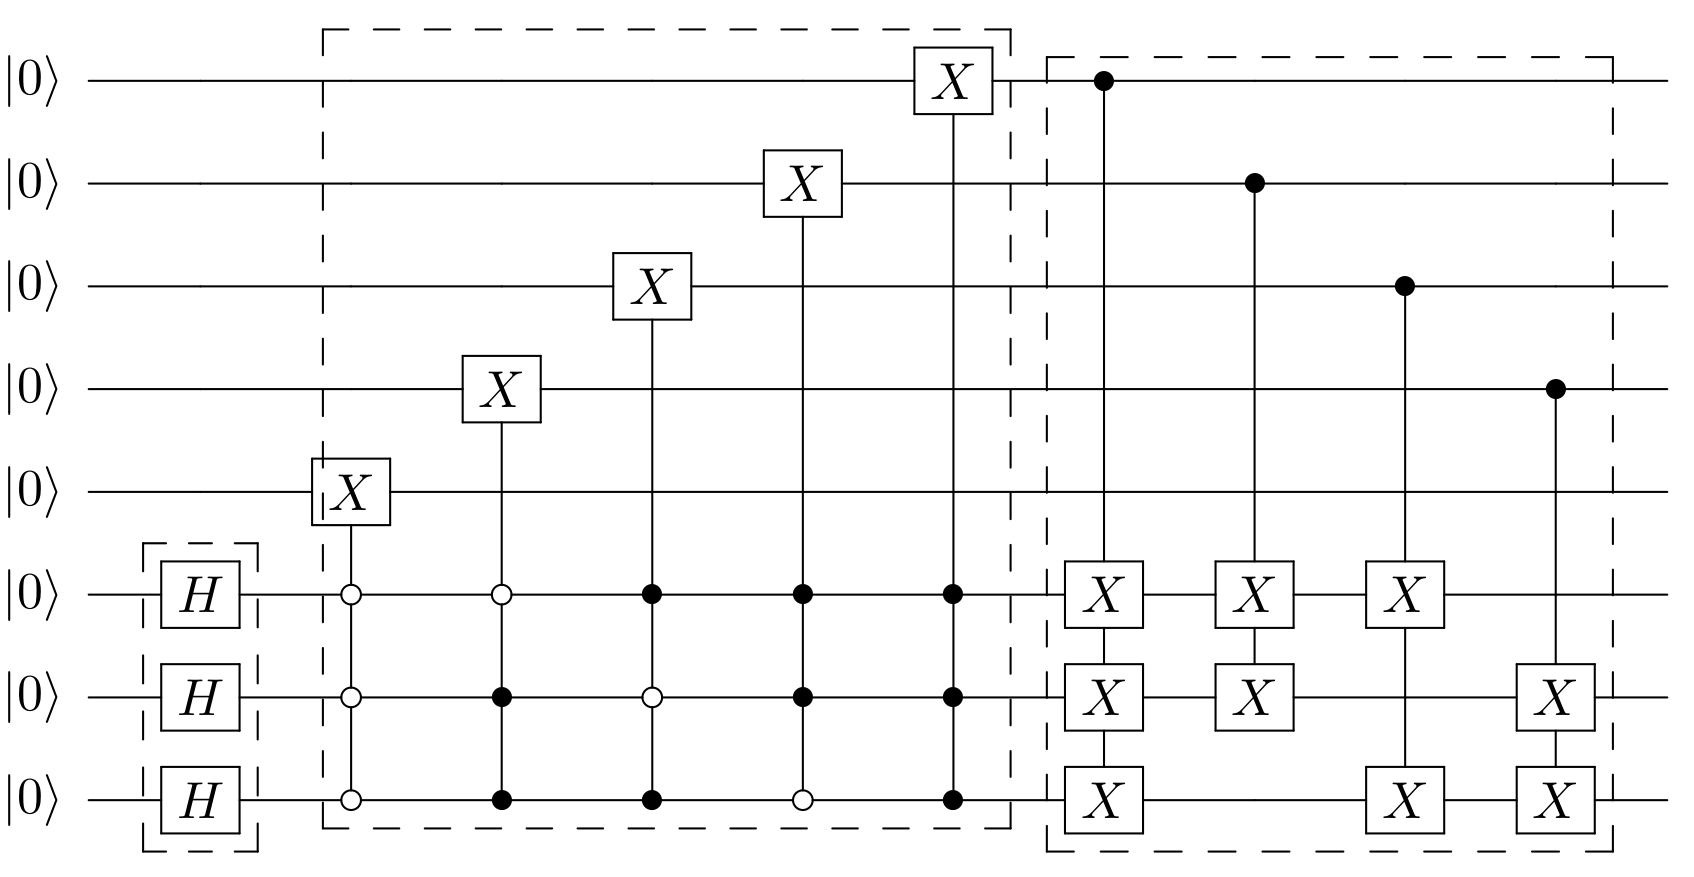
\includegraphics[width=0.8\linewidth]{pics/circuit-prepare-W-state-McClung.png}
\centering

\vspace{-.8em}

Circuit for computing the $\ket{W_8}$ state.

\vfill

\begin{theorem}[\cite{arunachalam2022parameterized}]
Any circuit which deterministically produces the
$\ket{W_n}$ state requires $\Omega(n)$ $T$ gates, unless ETH doesn't hold.
\end{theorem}

\vspace{-.5em}

\printbibliography[section=\therefsection]

\end{refsection}

\end{frame}





\begin{refsection}
\begin{frame}{\limdd Implementation}


\begin{exampleblock}{Circuit equivalence check implementation}
\begin{itemize}
	\item 	\limdd implemented in DDSIM~\cite{vinkhuijzen2023efficient}.
	\item 	Tested on QFT, after random Clifford  circuit
\end{itemize}
\end{exampleblock}


\vspace{-.5em}

\centering
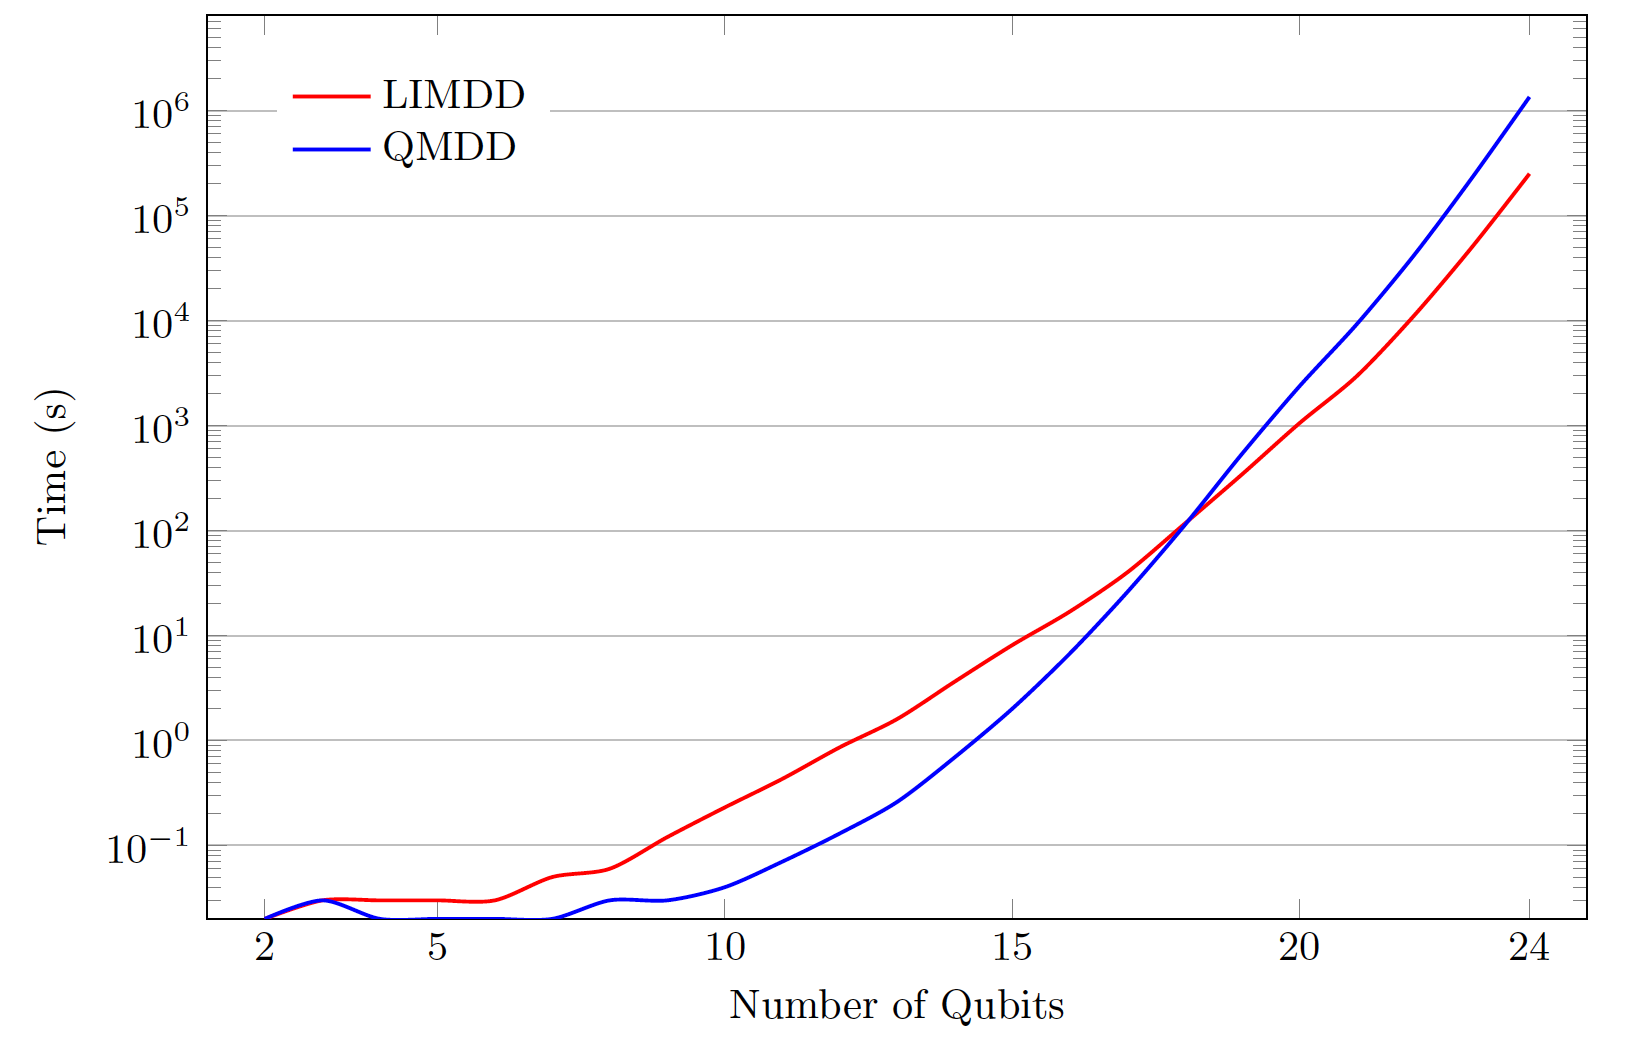
\includegraphics[height=5.cm]{plot.png}

\vspace{-.5em}

\centering
\printbibliography[section=\therefsection]
\vspace{-1em}
\url{https://github.com/cda-tum/mqt-limdd}

\end{frame}
\end{refsection}





 



\section{Quantum Information}


\begin{frame}
\begin{refsection}
	
\vfill

\vspace{-.5cm}\textbf{\Large A Knowledge Compilation Map for Quantum Information}~\cite{qkcm}\vspace{-.5cm}

\vfill

\printbibliography[section=\therefsection]
\end{refsection}

\end{frame}


\begin{frame}{Comparing Decision Diagrams vs RBM vs MPS}

\vspace{-.5em}
\centering

%\begin{figure}[b] 
~\begin{tikzpicture}[-{>[scale=0.3]},>=stealth',shorten >=1pt,auto,node distance=.4cm,
    thick, state/.style={circle,draw,minimum size=10pt,inner sep=.6pt},font=\scriptsize]

\node (vec) {
    \begin{minipage}{1.3cm}\footnotesize
$\def\arraystretch{1.}
    \begin{bmatrix*}[c]
    \frac1{\sqrt 2} \\ 0 \\ 0 \\ 0 \\ 0 \\ 0 \\ 0 \\ \frac1{\sqrt 2}
    \end{bmatrix*}
    $
    \end{minipage}
};


\node[state, right = 2cm of vec.north,anchor=north,yshift=-.2cm] (n1) {$x_3$};

\node[state](n2)[below = of n1, xshift=-.9cm]{$x_2$};
\node[state](n3)[below = of n1, xshift= .9cm]{$x_2$};

\node[state](n21)[below = of n2, ]{$x_1$};
\node[state](n22)[below = of n2, xshift= .9cm]{$x_1$};

\node[state](n31)[below = of n3]{$x_1$};

\node[draw, rectangle,minimum size=.5cm,below = of n21, xshift=.2cm,minimum size=10pt,inner sep=1pt] (l1) {$0$};
\node[draw, rectangle,minimum size=.5cm,right = of l1,minimum size=10pt,inner sep=1pt] (l2) {$\nicefrac1{\sqrt 2}$};


\path[]
(n1) edge[e1] node[right,pos=.7] {} (n3)
(n1) edge[e0] node[left,pos=.7] {} (n2)
(n2) edge[e0] node[left,pos=.7] {} (n21)
(n2) edge[e1] node[left,pos=.7] {} (n22)
(n3) edge[e0] node[left,pos=.7] {} (n22)
(n3) edge[e1] node[left,pos=.7] {} (n31)
(n21) edge[e0=  0]  node[pos=.7] {} (l2)
(n21) edge[e1=  0]  node[pos=.7] {} (l1)
(n22) edge[e0= 20]  node[pos=.7] {} (l1)
(n22) edge[e1= 20]  node[pos=.7] {} (l1)
(n31) edge[e0=  0]  node[pos=.7] {} (l1)
(n31) edge[e1=  0]  node[pos=.7] {} (l2)
;

\node[above=.5cm of n1,anchor=north]    (add) {\textbf{\add}};
\node[left =1.3cm of add]    (svc) {\textbf{Vector}};


\node[state, right=2cm of n1] (q1) {$x_3$} ;
\node[state, below=of q1,xshift=-0.5cm] (q2) {$x_2$} ;
\node[state, below=of q1,xshift=0.5cm] (q3) {$x_2$} ;
\node[state, below=of q2] (q4) {$x_1$} ;
\node[state, below=of q3] (q5) {$x_1$} ;
\node[draw, rectangle,minimum size=.5cm,below = of q4,xshift=0.5cm,minimum size=10pt,inner sep=1pt] (l1) {$1$};


\draw[e0] (q1) edge  node[] {} (q2);
\draw[e1] (q1) edge  node[] {} (q3);
\draw[e0=25] (q2) edge  node[] {} (q4);
\draw[e1=25] (q2) edge  node[,pos=.45] {$0$} (q4);
\draw[e0=25] (q3) edge  node[] {} (q5);
\draw[e1=25] (q3) edge  node[,xshift=-0.6cm,pos=.45] {$0$} (q5);
\draw[e0=-20] (q4) edge  node[] {} (l1);
\draw[e1=-20] (q4) edge  node[,left=.1cm,pos=.45] {$0$} (l1);
\draw[e0=-20] (q5) edge  node[] {} (l1);
\draw[e1=-20] (q5) edge  node[,xshift=0.4cm,pos=.45] {$0$} (l1);
\draw[<-] (q1) --++(90:.5cm) node[right=.2cm,pos=.7,] {$\nicefrac 1{\sqrt 2}$} node[right,pos=.8] {};

\node[right =1.7cm of add]    (sldd) {\textbf{QMDD}};



    \node[state, right = 1.8cm of q1] (a1) {$x_3$};
    \node[state, below = of a1] (a3) {$x_2$};
    \node[state, below = of a3] (a4) {$x_1$};
    \node[draw,rectangle,minimum size=0.5cm, below= of a4,minimum size=10pt,inner sep=1pt] (w4) {1};


    \draw[<-] (a1) --++(90:.5cm) node[right=.2cm,pos=.7,] {$\nicefrac 1{\sqrt 2} \cdot \id^{\otimes3}$} node[left,pos=.8] {};
    \draw[e0=25] (a1) edge  node[] {} (a3);
    \draw[e1=25] (a1) edge  node[pos=.3,right] {$X \otimes X$} (a3);
    \draw[e0=25] (a1) edge  node[] {} (a3);
    \draw[e1=25] (a3) edge  node[pos=.3,right] {$0$} (a4);
    \draw[e0=25] (a3) edge  node[] {} (a4);
    \draw[e0=25] (a4) edge  node[] {} (w4);
    \draw[e1=25] (a4) edge  node[pos=.3,right] {0} (w4);

\node[right=1.4cm of sldd]    (limdd) {\textbf{\limdd}};


%\pause

\node[state, xshift=-5cm, below=.7cm of l1,yshift=.cm] (h1) {$h_1$} ;
\node[state, right=.65cm of h1] (h2) {$h_2$} ;
\node[state, right=.65cm of h2] (h3) {$h_3$} ;
\node[state, right=.65cm of h3] (h4) {$h_4$} ;
\node[state, below=1.7cm of h1, xshift=0.5cm] (v1) {$v_1$} ;
\node[state, right=.7cm of v1] (v2) {$v_2$} ;
\node[state, right=.7cm of v2] (v3) {$v_3$} ;


\draw[e1] (h1) edge  node[] {} (v1);
\draw[e1=-10] (h1) edge  node[] {} (v2);
\draw[e1=-10] (h1) edge  node[] {} (v3);
\draw[e1=10] (h2) edge  node[] {} (v1);
\draw[e1] (h2) edge  node[] {} (v2);
\draw[e1=-10] (h2) edge  node[] {} (v3);
\draw[e1=10] (h3) edge  node[] {} (v1);
\draw[e1] (h3) edge  node[] {} (v2);
\draw[e1=-10] (h3) edge  node[] {} (v3);
\draw[e1=10] (h4) edge  node[] {} (v1);
\draw[e1=10] (h4) edge  node[] {} (v2);
\draw[e1] (h4) edge  node[] {} (v3);


\node[draw,rectangle, below=0.2cm of h1, fill=white, opacity=1] (1) {$i\pi/3$};
\node[draw,rectangle, below=0.2cm of h2, fill=white, opacity=1] (1) {$i\pi/3$};
\node[draw,rectangle, below=0.2cm of h3, xshift=-0.2cm, fill=white, opacity=1] (1) {$-i\pi/3$};
\node[draw,rectangle, below=0.2cm of h4, fill=white, opacity=1] (1) {$-i\pi/3$};


\node[above=0.cm of h3,xshift=-0.6cm]    (a31) {{hidden layer}};
\node[below=0.cm of v2,xshift=0.1cm]    (a31) {{visible layer}};

\node[below=.2cm of l1,xshift=-3.3cm]    (rbm) {\textbf{RBM}};



\node[right=.7cm of h4] (a30) {$A_3^0=\begin{bmatrix}1 & 0\end{bmatrix}$};
\node[right=2cm of a30.west, anchor=west]   (a31) {$A_3^1=\begin{bmatrix}0 & 1\end{bmatrix}$};
\node[below=1.cm of a30.west, anchor=west] (a20) {$A_2^0=\begin{bmatrix}1 & 0 \\ 0 & 0\end{bmatrix}$};
\node[below=1.cm of a31.west, anchor=west] (a21) {$A_2^1=\begin{bmatrix}0 & 0 \\ 0 & 1\end{bmatrix}$};
\node[below=1.cm of a20.west, anchor=west] (a10) {$A_1^0=\begin{bmatrix}\frac1{\sqrt 2} \\ 0\end{bmatrix}$};
\node[below=1.cm of a21.west, anchor=west] (a11) {$A_1^1=\begin{bmatrix}0 \\ \frac1{\sqrt 2}\end{bmatrix}$};

\node[right=3.8cm of rbm]    (a31) {\textbf{MPS}};



\end{tikzpicture}

%\caption{The $3$-qubit GHZ state $\nicefrac{1}{\sqrt 2}(\ket{000} + \ket{111})$, displayed using different data structures.
%The unlabelled edges for \add, \qmdd, \limdd have resp. label 1, 1, $\id$.
%In the RBM, the weights of edges incident to $h_1,h_2$ ($h_3, h_4$) are all $i\pi/3$ ($-i\pi/3$); the hidden node biases $(\beta_{h_1}, \beta_{h_2}, \beta_{h_3}, \beta_{h_4}) = i\pi \cdot (1/3, 2/3, -1/3, -2/3)$; the visible node biases $\alpha_{v_1}=\alpha_{v_2}=\alpha_{v_3}=0$.
%}
%\label{fig:ghz-examples}
%\end{figure}

\pause

\begin{block}{Compare Different Representations Analytically}
	\begin{itemize}\vspace{-.5em}
		\item \textbf{Succinctness}: Families of quantum states showing exponential separations
		\item \textbf{Tractability}: Is manipulation of the representation (e.g., applying a gate) efficient
	\end{itemize}\vspace{-.5em}
\end{block}

\end{frame}




\begin{frame}{Matrix Product States}

\begin{definition}[MPS on $n$ qubits]
	An MPS $M$ is a series of $2n$ matrices of the right dimensions.
	\vspace{.5em}
	
	$A_1^0,~~~ A_2^0,~~~ \dots,~~~ A_n^0$\\
	\vspace{.5em}
	$A_1^1,~~~ A_2^1,~~~ \dots,~~~ A_n^1$
	
	\vspace{.5em}

The interpretation $\ket{M}$ is determined as $\braket{\vec x | M} = A_n^{x_n} \cdot  \cdots  \cdot A_2^{x_2}  \cdot A_1^{x_1}$ for $\vec x \in \{0, 1\}^n$.
\end{definition}

\pause

\begin{exampleblock}{MPS}
	\begin{tikzpicture}[-{>[scale=0.3]},>=stealth',shorten >=1pt,auto,node distance=.4cm,
    thick, state/.style={circle,draw,minimum size=10pt,inner sep=.6pt},font=\scriptsize]

\node (vec) {
    \begin{minipage}{1.3cm}\footnotesize
$\def\arraystretch{1.}
    \begin{bmatrix*}[c]
    \frac1{\sqrt 2} \\ 0 \\ 0 \\ 0 \\ 0 \\ 0 \\ 0 \\ \frac1{\sqrt 2}
    \end{bmatrix*}
    $
    \end{minipage}
};


\node[right=.7cm of vec, yshift=1cm] (a30) {$A_3^0=\begin{bmatrix}1 & 0\end{bmatrix}$};
\node[right=2cm of a30.west, anchor=west]   (a31) {$A_3^1=\begin{bmatrix}0 & 1\end{bmatrix}$};
\node[below=1.cm of a30.west, anchor=west] (a20) {$A_2^0=\begin{bmatrix}1 & 0 \\ 0 & 0\end{bmatrix}$};
\node[below=1.cm of a31.west, anchor=west] (a21) {$A_2^1=\begin{bmatrix}0 & 0 \\ 0 & 1\end{bmatrix}$};
\node[below=1.cm of a20.west, anchor=west] (a10) {$A_1^0=\begin{bmatrix}\frac1{\sqrt 2} \\ 0\end{bmatrix}$};
\node[below=1.cm of a21.west, anchor=west] (a11) {$A_1^1=\begin{bmatrix}0 \\ \frac1{\sqrt 2}\end{bmatrix}$};


\end{tikzpicture}

\end{exampleblock}

	
\end{frame}


\begin{frame}{QMDD vs MPS}


\begin{theorem}
MPS is at least as succinct as QMDD.	
\end{theorem}


\pause

\textbf{Proof:} 

\centering
	\begin{tikzpicture}[-{>[scale=0.3]},>=stealth',shorten >=1pt,auto,node distance=.4cm,
    thick, state/.style={circle,draw,minimum size=10pt,inner sep=.6pt},font=\scriptsize]


\node[yshift=1cm] (a30) {$A_3^0=\begin{bmatrix}1 & 0\end{bmatrix}$};
\onslide<+(1)->{
\node[right=2cm of a30.west, anchor=west]   (a31) {$A_3^1=\begin{bmatrix}0 & 1\end{bmatrix}$};
}
\node[below=1.cm of a30.west, anchor=west] (a20) {$A_2^0=\begin{bmatrix}1 & 0 \\ 0 & 0\end{bmatrix}$};
\onslide<.(1)->{
\node[below=1.cm of a31.west, anchor=west] (a21) {$A_2^1=\begin{bmatrix}0 & 0 \\ 0 & 1\end{bmatrix}$};
}
\node[below=1.cm of a20.west, anchor=west] (a10) {$A_1^0=\begin{bmatrix}\frac1{\sqrt 2} \\ 0\end{bmatrix}$};
\onslide<.(1)->{
\node[below=1.cm of a21.west, anchor=west] (a11) {$A_1^1=\begin{bmatrix}0 \\ \frac1{\sqrt 2}\end{bmatrix}$};
}


\node[state, right=2cm of a31] (q1) {$x_3$} ;
\node[state, below=of q1,xshift=-0.5cm] (q2) {$x_2$} ;
\node[state, below=of q1,xshift=0.5cm] (q3) {$x_2$} ;
\node[state, below=of q2] (q4) {$x_1$} ;
\node[state, below=of q3] (q5) {$x_1$} ;
\node[draw, rectangle,minimum size=.5cm,below = of q4,xshift=0.5cm,minimum size=10pt,inner sep=1pt] (l1) {$1$};


\draw[e0] (q1) edge  node[] {} (q2);
\onslide<.(1)->{
\draw[e1] (q1) edge  node[] {} (q3);
}
\draw[e0=25] (q2) edge  node[] {} (q4);
\onslide<.(1)->{
\draw[e1=25] (q2) edge  node[,pos=.45] {$0$} (q4);
}
\draw[e0=25] (q3) edge  node[] {} (q5);
\onslide<.(1)->{
\draw[e1=25] (q3) edge  node[,xshift=-0.6cm,pos=.45] {$0$} (q5);
}
\draw[e0=-30] (q4) edge  node[above ] {$\frac 1{\sqrt 2}$} (l1);
\onslide<.(1)->{
\draw[e1=-20] (q4) edge  node[,left=.1cm,pos=.45] {$0$} (l1);
}
\draw[e0=-40] (q5) edge  node[right] {$0$} (l1);
\onslide<.(1)->{
\draw[e1=-20] (q5) edge  node[above,xshift=0.cm,pos=.45] {$\frac 1{\sqrt 2}$} (l1);
}
\draw[<-] (q1) --++(90:.5cm) node[right=.2cm,pos=.7,] {} node[right,pos=.8] {};

%\node[right =1.7cm of add]    (sldd) {\textbf{QMDD}};

\end{tikzpicture}

	
\end{frame}



\begin{frame}{\limdd vs MPS}


\begin{lemma}
	There is a family of quantum states with polynomial-size \limdd but exponential-size MPS.
\end{lemma}

\vspace{-.5em}

\textbf{Proof:} It is well-known that MPS can be exponentially sized for stabilizer states.


\vspace{.5em}

\pause


\begin{lemma}
	There is a family of quantum states with polynomial-size MPS but exponential-size \limdd.
\end{lemma}


\vspace{-.5em}
\textbf{Proof sketch:} 

Take the state: \vspace{-2.5em}
\begin{align}
\sumstate = \ket{+}^{\otimes n} + \bigotimes_{j=1}^n(\ket 0+e^{i\pi 2^{-j-1}}\ket 1)
\end{align}
MPS: \vspace{-2.5em}
\begin{align*}
	    A^{0}_1 = \begin{bmatrix} 1 & 1\end{bmatrix}, ~~~~  &A^{x_j}_j = \begin{bmatrix} 1 &  0 \\ 0 & 1 \end{bmatrix}, ~~~~~~ &&A^{x_n}_n = \begin{bmatrix} 1 \\ 1\end{bmatrix}&\\
	    A^{x_1}_1 = \begin{bmatrix} 1 & e^{i\pi 2^{-2}}\end{bmatrix}, ~~~~  &A^{x_j}_j = \begin{bmatrix} 1 &  0 \\ 0 & \prod_{j=2}^{n-1}e^{i\pi 2^{-j-1}}\end{bmatrix},  && A^{x_n}_n = \begin{bmatrix} 1 \\ e^{i\pi 2^{-n-1}}&\end{bmatrix},
	\end{align*}	

LIMDD: There is no LIM mapping subfunctions $f_{\vec a}$ 
to each other for different ${\vec a}$
\[
f_{\vec a}(x_1) = 1 + e^{i\pi \sum_{j=2}^n a_j \cdot 2^{-j-1}} \cdot
e^{i\pi \cdot \nicefrac14 x_1 }.
\]

\end{frame}



\begin{frame}{\limdd vs RBM}
\begin{refsection}


\begin{lemma}
	There is a family of quantum states with polynomial-size RBM but exponential-size \limdd.
\end{lemma}

%\textbf{Proof:}
%
%\begin{columns}[T]
%\begin{column}{0.6\textwidth}
%We use the seminal Boolean function $IP:  \vec{x}, \vec{y} \mapsto  \vec{x}^T  \vec{y} \mod 2$ for even $n$, which computes the inner product between the first half of the input with the second half.
%
%~\\
%
%\citeauthor{martens2013representational}~\cite{martens2013representational} shows RBM is exponential for it.
%\end{column}
%\begin{column}{0.3\textwidth}
%\vspace{-3em}
%\scalebox{.5}{
%\begin{tikzpicture}[
%    scale=0.3,
%    every path/.style={>=latex},
%    every node/.style={},
%    inner sep=0pt,
%    minimum size=14pt,
%    line width=1pt,
%    node distance=.3cm,
%    thick,
%    font=\footnotesize
%    ]
%
%    \node[] (root)   {};
%    \node[draw,circle, below =of root, xshift=0cm] (l1) {};
%    \node[draw,circle, below =of l1] (l2) {};
%
%    \node[draw,circle, below =of l1, xshift=1cm] (ma2) {};
%
%    \node[draw,circle, below =of l2] (l3) {};
%    \node[draw,circle, below =of l2, xshift=3cm] (r3) {};
%    \node[draw,circle, below =of l3] (l4) {};
%    \node[draw,circle, below =of r3] (r4) {};
%    \node[draw,circle, below =of l3, xshift=1cm] (ma4) {};
%    \node[draw,circle, below =of l3, xshift=2cm] (mb4) {};
%
%    \node[draw,circle, below =.6cm of l4] (l5) {};
%    \node[draw,circle, below =.6cm of r4] (r5) {};
%
%    \node[draw,circle, below= of l5] (l6) {};
%    \node[draw,circle, below= of r5] (r6) {};
%    \node[draw,circle, below= of l5, xshift=1cm] (ma6) {};
%    \node[draw,circle, below= of l5, xshift=2cm] (mb6) {};
%
%	 \node[left of =l1] 	{$x_1$};
%	 \node[left of =l2] 	{$x_2$};
%	 \node[left of =l3] 	{$x_3$};
%	 \node[left of =l4] 	{$x_4$};
%	 \node[left  =.1cm of l5] 	{$x_{n-1}$};
%	 \node[left of =l6] 	{$x_{n}$};
%
%    \node[draw,circle,rectangle,minimum size=0.4cm, below=of l6] (leaf0) {$0$};
%    \node[draw,circle,rectangle,minimum size=0.4cm, below=of r6] (leaf1) {$\frac{1}{A}$};
%
%    \draw[<-] (l1) --++(90:2cm) node[pos=1.4,right] {};
%
%    \draw[e0=0] (l1) edge  node[] {} (l2);
%    \draw[e1=0] (l1) edge  node[] {} (ma2);
%
%
%    \draw[e0=25] (l2) edge  node {} (l3);
%    \draw[e1=25] (l2) edge  node {} (l3);
%
%
%    \draw[e0=0] (ma2) edge  node {} (l3);
%    \draw[e1=0] (ma2) edge  node {} (r3);
%
%
%    \draw[e0=0] (l3) edge  node {} (l4);
%    \draw[e1=0] (l3) edge  node {} (ma4);
%
%    \draw[e1=0] (r3) edge  node {} (mb4);
%    \draw[e0=0] (r3) edge  node[left] {} (r4);
%
%    \node[ xshift=0.5cm, yshift=.5cm, below= of ma4] (a) {$\pmb{\vdots}$};
%
%    \draw[e0=0] (l5) edge  node {} (l6);
%    \draw[e1=0] (l5) edge  node {} (ma6);
%
%    \draw[e0=0] (r5) edge  node {} (r6);
%    \draw[e1=0] (r5) edge  node {} (mb6);
%
%    \draw[e0=0] (ma6) edge  node {} (leaf0);
%    \draw[e1=0] (ma6) edge  node {} (leaf1);
%
%    \draw[e0=0] (mb6) edge  node {} (leaf1);
%    \draw[e1=0] (mb6) edge  node {} (leaf0);
%
%    \draw[e0=25] (l6) edge  node {} (leaf0);
%    \draw[e1=25] (l6) edge  node {} (leaf0);
%
%    \draw[e1=25] (r6) edge  node {} (leaf1);
%    \draw[e0=25] (r6) edge  node {} (leaf1);
%\end{tikzpicture}
%}
%\end{column}
%\end{columns}

	
%\onslide<+->{


\begin{lemma}
	There is a family of quantum states with polynomial-size \limdd but exponential-size RBM.
\end{lemma}

%We use the $\ket{Sum}$ state again.
%}

%\printbibliography[section=\therefsection]
\end{refsection}
\end{frame}



\begin{refsection}
\begin{frame}{A Knowledge Compilation Map for Quantum Information}

\begin{theorem}[Decision Diagram vs MPS vs RBM~\cite{qkcm}]
\begin{itemize}
%	\item is a generalization of QMDD
%	\item Nodes are merged up to $\gamma \cdot P_1 \otimes \dots \otimes P_n$ with $P_1, \dots, P_n \in \set{\id, X, Y, Z}$
%	\item<2-> All stabilizer states have linear \limdd size
%	\item<3-> Stabilizer (Clifford) circuit simulation is polynomial time in \limdd
%\pause
%\pause
%	\item RBM is quantum neural network
%	\item MPS is a tensor train (linear tensor network)
	\item<+-> \limdd \& MPS are exponentially more succinct than QMDD \& ADD
	\item<+-> \limdd, MPS \& RBM are incomparable
	\item<+-> Some operations become harder on \limdd
\end{itemize}

\centering

\begin{columns}%[onlywidth,T]
	\begin{column}{.35\textwidth}
\phantom{ZZZZ}
\scalebox{.63}{
\hspace{2em}
\begin{tikzpicture}[node distance=.7cm,minimum height=.5cm]
        % nodes
		\node[draw] (mps) 			   {MPS};
		\node[draw, right =2cm of mps, yshift=-2.1cm] (limdd) {\limdd};
%		\node[draw, above =of limdd, yshift=1.5cm] (tn) {TN};
\onslide<2->{
		\node[draw, right =2cm of limdd, yshift=2.1cm] (rbm) {RBM};
}
%		\node[draw, below =2cm of rbm, xshift=0.4cm,text width=1.3cm, align=center] (ss) {Stabilizer States};
		\node[draw, below = 1cm of limdd] (qmdd) {QMDD};
		\node[draw, below = 1cm of qmdd] (add) {ADD};
%		\node[draw, below = 1cm of add, xshift= 0cm] (statevec) {Vector};

        % edges MPS
\onslide<2->{

		\draw[\bigarrowheadb, bend left=0] (limdd.north west) to[<->] node[midway] {$\boldsymbol{\bigtimes}$} 
											node[pos=.8,right] {\supp{\autoref{thm:succ-limdd-vs-mps}}}
											node[pos=.2,right] {\supp{\autoref{thm:succ-mps-vs-limdd}}}
											(mps.south east);
}

		\draw[\bigarrowhead, bend left=-10] (mps) to (qmdd.west);

		\draw[\bigarrowhead, bend left=-20] (mps.south west) to
													 (add.west);

\onslide<2->{

        % edges RBM
		\draw[\bigarrowheadb, bend left=0] (rbm.west) to node[midway] {$\boldsymbol{\bigtimes}$} 
											(mps.east);

		\draw[\bigarrowheadb, bend right=0] (rbm.south west) to node[midway] {$\boldsymbol{\bigtimes}$} 
											node[pos=.7,above left=-1mm] {\supp{\autoref{thm:succ-rbm-vs-limdd}}} 
											(limdd.north east);

		\draw[\bigarrowheadb, bend left=10] (rbm) to node[midway] {$\boldsymbol{\bigtimes}$} 
										   (qmdd.east);

		\draw[\bigarrowheadb, bend left=20] (rbm.south east) to node[midway] {$\boldsymbol{\bigtimes}$}
											node[pos=.3,below right=-1mm] {\supp{\autoref{thm:add-rbm}}} 
											 (add.east);
}


		%edges QDD
		\draw[\bigarrowhead, bend right=0] (limdd) to (qmdd);
		\draw[\bigarrowhead, bend right=0] (qmdd) to  (add);

	\end{tikzpicture}
}
\footnotesize
\\
\hspace{3em}
~~~~~~Succinctness separations.
%\phantom{ZZ}
%\phantom{ZZ}\begin{tikzpicture}\footnotesize
%  \tikzset{venn circle/.style={circle,minimum width=2cm,fill=####1,opacity=0.4}}
%  \node [venn circle=white,minimum width=4cm,draw] (A) at (0,0.3) {};
%  \node  at (0,1.95) 			{State space};
%
%  \node [venn circle = Red!40!white, ellipse,minimum height=2.2cm, minimum width=3.6cm] (L) at (0,0.6) {};
%  \node  at (0,1.5) 		{\limdd};
%  
%  \node [venn circle = blue!70!white,text width=1.3cm,align=center,rotate=79,ellipse,minimum height=1.8cm, minimum width=2.5cm] (B) at (-.6,-.2) {};
%  \node[text width=1.3cm,align=center]  at (-.9,-1.) {MPS};
%
%
%  \node [venn circle = green!70!white,text width=1.3cm,align=center,rotate=119,ellipse,minimum height=1.8cm, minimum width=2.5cm] (B) at (.6,-.2) {};
%  \node[text width=1.3cm,align=center]  at (.9,-1.) {RBM};
%
%
%
%  \node [venn circle = Blue!100!white,text width=1cm,align=center, minimum width=1.cm] (B) at (-.5,.3) 	{\textcolor{white}{QMDD}};						
%
%  \node [venn circle = OliveGreen!100!white,text width=1cm,align=center, minimum width=1.cm] (C) at (.5,.2) {\textcolor{white}{Stabilizer states}};
%
%\end{tikzpicture}
	\end{column}
	\begin{column}{.65\textwidth}
\onslide<3->{
\setlength{\tabcolsep}{2pt}
\def\arraystretch{1.1}
\footnotesize
\centering
\begin{tabular}{|l@{\hspace{10pt}}|| *{5}{c|}| *{20}{c|}}
%\footnotesize
\hline
 & \multicolumn{5}{c||}{Queries} & \multicolumn{7}{c|}{Manipulation operations} \\
	& \rot{\samp} & \rot{\pro} & \rot{\eq}  & \rot{\inprod} & \multicolumn{1}{R{90}{0em}||}{\fid}
	& \rot{\addi} & \rot\had & \rot{\xyz} & \rot\cz & \rot{\swap} & \rot{\loc} & \rot{\T-gate} \\
\hline
Vector& \Yar & \Yes & \Yes & \Yes & \Yes & \Yes & \Yes & \Yes & \Yes & \Yes & \Yes & \Yes \\
\hline
%		| Sampl	| Prob 	| Eq	|Inprod	| Fid
ADD   	& \Yar	& \Yes	& \Yes	& \Yes & \Yes
%		| Add	| H		| XYZ	| CX	| Swap	| Local	| T
		& \Yes	& \Yes 	& \Yes	& \Yes	& \Yes	& \Yes	& \Yes \\
\hline
QMDD
		& \Yar	& \Yes	& \Yes	& \Yes & \Yes
		& \No	& \No 	& \Yes	& \Yes	& \No	& \No	& \Yes \\
\hline 
%QMDD  & \Yes & \Yes & \Yes & \No & \Yes & \No & ?? & ??  & ?? & \No & ?? & ??   \\
%\hline    
\limdd 	& \Yar	& \Yes	& \Yes	& \Cond & \Cond
		& \No	& \No	& \Yes	& \Yes	& \No	& \No	& \Yes  \\
\hline 
%TN    & \Cond? & \Cond? & \Cond? & \Cond? & ?? & \Yes? & \Yes? & \Yes? & \Yes? & \Yes? & \Yes? \\ \hline
MPS   & \Yar & \Yes & \Yes & \Yes & \Yes & \Yes 
	  & \Yes & \Yes & \Yes & \Yes & \Yes & \Yes  \\
\hline 
RBM   & \Yar    & ? & ? & \Cond & \Cond & ? & ? & \Yes & \Yes & \Yes & ? & \Yes \\
\hline 
%\multicolumn{13}{c}{Low priority} \\
%\hline 
%ZX    & ?? & ?? & ?? & ?? & ?? & ?? & ?? & ?? & ?? & ?? & ?? & ?? \\
%\hline 
%SLDD$_+$  & \Yes? & \Yes? & \Yes? & \Yes? & \Yes? & \No! & \No? & \Yes? & \No! & \No! & \No? & \Yes! \\
%\hline 
\end{tabular}
%\captionof{table}{
%From \cite{qkr2023}: Tractability of various queries and transformations on the data structures analyzed in this paper (single application of the operation). 
%\Yes means the data structure supports the operation in polytime,\\
%\Yar means supported in randomized polytime, and 
\footnotesize
\\
\hspace{-1.em}
\Yes(\No) means the operation is (not) supported in polytime.
\\
\phantom{ZZ}
\Cond means the operation is not supported unless $P=NP$.
%? is unknown.
%%\textbf{Fidelity} (not shown) has the same tractability as \textbf{Inprod} for all data structures considered.
%%\todo[inline]{still true?}
%The table only considers deterministic algorithms (for some ? a probabilistic algorithm exists, e.g., for \inprod on RBM).
%}
%\label{tab:tractability}
}
	\end{column}
\end{columns}
\vspace{1em}
\vspace{-1em}
\end{theorem}


\printbibliography[section=\therefsection]

\end{frame}
\end{refsection}




\begin{refsection}
\begin{frame}{Fidelity}
	\begin{theorem}
		RBM and \limdd are not tractable for \textbf{Fidelity}, unless ETH fails.
	\end{theorem}

\textbf{Proof:}
Let $\ket{D^k_n}$ be the Dicke state on $n$ qubits where all non-zero amplitudes have Hamming weight $k$.

Let $G_n$ be an $n$-vertex graph and $\ket{G_n}$ be the corresponding graph state.

\alert{The \#EVEN SUBGRAPHS problem reduces to computing the fidelity $\braket{D^k_n| G_n}$}


\begin{definition}[\#EVEN SUBGRAPHS]
	\textbf{Input:} A graph $G=(V,E)$, an integer $k$\\
	\textbf{Output:} The number of induced $k$-vertex subgraphs with an even number of edges
\end{definition}


\begin{theorem}[\citeauthor{jerrum2017parameterised}]
	\label{thm:even-subgraphs-ETH-hard}
	If \#EVEN SUBGRAPHS is not in \P, unless ETH is false.
\end{theorem}

\onslide<2>{\alert{Actually, omitting detail: \#EVEN-ODD-SUBGRAPH-DIFFERENCE}}

\printbibliography[section=\therefsection]

\end{frame}
\end{refsection}





\begin{frame}{Circuit Simulation vs Applying Individual Gates}


\begin{alertblock}{Downsides of operation tractability}
	\begin{itemize}
	\item Only compares worst cases.
	\begin{itemize}
	\item ADD is tractable for all gates
	\item QMDD is intractable for e.g. Hadamard
	\item However, there is no state for which QMDD takes longer than ADD!
	\end{itemize}
	\item<+-> It tells us nothing about circuit simulation.
\begin{itemize}
	\item The circuit might double at every step.
%	\item 
\end{itemize}
	\end{itemize}
\end{alertblock}


\setlength{\tabcolsep}{2pt}
\def\arraystretch{1.1}
\footnotesize
%\centering
\begin{tabular}{|l@{\hspace{10pt}}|| *{5}{c|}| *{20}{c|}}
%\footnotesize
\hline
 & \multicolumn{5}{c||}{Queries} & \multicolumn{7}{c|}{Manipulation operations} \\
	& \rot{\samp} & \rot{\pro} & \rot{\eq}  & \rot{\inprod} & \multicolumn{1}{R{90}{0em}||}{\fid}
	& \rot{\addi} & \rot\had & \rot{\xyz} & \rot\cz & \rot{\swap} & \rot{\loc} & \rot{\T-gate} \\
\hline
Vector& \Yar & \Yes & \Yes & \Yes & \Yes & \Yes & \Yes & \Yes & \Yes & \Yes & \Yes & \Yes \\
\hline
%		| Sampl	| Prob 	| Eq	|Inprod	| Fid
ADD   	& \Yar	& \Yes	& \Yes	& \Yes & \Yes
%		| Add	| H		| XYZ	| CX	| Swap	| Local	| T
		& \Yes	& \Yes 	& \Yes	& \Yes	& \Yes	& \Yes	& \Yes \\
\hline
QMDD
		& \Yar	& \Yes	& \Yes	& \Yes & \Yes
		& \No	& \No 	& \Yes	& \Yes	& \No	& \No	& \Yes \\
\hline 
%QMDD  & \Yes & \Yes & \Yes & \No & \Yes & \No & ?? & ??  & ?? & \No & ?? & ??   \\
%\hline    
\limdd 	& \Yar	& \Yes	& \Yes	& \alert{\Cond} & \alert{\Cond}
		& \No	& \No	& \Yes	& \Yes	& \No	& \No	& \Yes  \\
\hline 
%TN    & \Cond? & \Cond? & \Cond? & \Cond? & ?? & \Yes? & \Yes? & \Yes? & \Yes? & \Yes? & \Yes? \\ \hline
MPS   & \Yar & \Yes & \Yes & \Yes & \Yes & \Yes 
	  & \Yes & \Yes & \Yes & \Yes & \Yes & \Yes  \\
\hline 
RBM   & \Yar    & ? & ? & \alert{\Cond} & \alert{\Cond} & ? & ? & \Yes & \Yes & \Yes & ? & \Yes \\
\hline 
%\multicolumn{13}{c}{Low priority} \\
%\hline 
%ZX    & ?? & ?? & ?? & ?? & ?? & ?? & ?? & ?? & ?? & ?? & ?? & ?? \\
%\hline 
%SLDD$_+$  & \Yes? & \Yes? & \Yes? & \Yes? & \Yes? & \No! & \No? & \Yes? & \No! & \No! & \No? & \Yes! \\
%\hline 
\end{tabular}

\vspace{-.5em}
\footnotesize
\Yes means supported in (randomized \Yar) polytime\\
% means supported in randomized polytime, and 
\No means (not) supported in polytime
\\
\Cond means not supported in polytime conditionally

\end{frame}



\begin{frame}{Rapidity for Non-Canonical Data Structures}
\begin{refsection}

\vspace{-.5em}

\begin{itemize}
	\item Rapidity compares performance of operations on individual states
	\item Invented by Lai, Liu and Yin~\cite{lai2017new}
	\item We provide a more general definition
\end{itemize}


\begin{theorem}[\alert{omitting details}]
	If there is a polynomial time translation from data structure $D_1$ to $D_2$ and back, 
	
	and if there is a runtime monotonic algorithm implementing OP,
	
	then almost all operations on $D_1$ can be done as fast as on $D_2$.
\end{theorem}

\vspace{-.5em}
\centering

\scalebox{.75}{
 \begin{tikzpicture}[ele/.style={fill=black,circle,minimum width=.8pt,inner sep=1pt},every fit/.style={ellipse,draw,inner sep=-2pt}]


  \node[ele,label=left:$x_1$] (x1) at (0,2.5) {};    
	 \node[ele] (a1) at (0,1) {};

  \node[ele,,label=left:$x_2$] (x2) at (6.5,2.5) {};
  \node[ele,,label=right:$f(x_1)$] (fx1) at (4,2.5) {};
	 \node[ele,] (a2) at (6.5,1) {};
	 \node[ele,] (a2prime) at (4,1) {};

  \node[draw,gray!60,fit= (x1) (a1) ,minimum width=2cm,minimum height=3cm, label={above:$D_1$}] {};] {} ;
  \node[draw,gray!60,fit= (x2) (fx1) (a2prime) (a2),minimum width=5cm, minimum height=3cm,label={above:$D_2$}] {};]] {} ;

	 \draw[->,bend left=20,thick,shorten <=2pt,shorten >=2pt] (x1) to node[midway,fill=white] {$f$} (fx1);
  \draw[->,thick,shorten <=2pt,shorten >=2pt] (fx1) to node[midway,fill=white,solid] {$ALG_2^{rm}$} (a2prime);
  \draw[->,thick,shorten <=2pt,shorten >=2pt] (x2) to node[midway,fill=white,solid] {$ALG_2$} (a2);
	 \draw[->,bend left=20,thick,shorten <=2pt,shorten >=2pt] (a2prime) to node[midway,fill=white,solid] {$g$} (a1);

 \end{tikzpicture}
 }

\onslide<+->{
\centering

\renewcommand\qmdd{QMDD}


\centering
\scalebox{.7}{
	\begin{tikzpicture}[node distance=.5cm,minimum height=.5cm]

		\node[draw] (mps) 			   {MPS};
		\node[draw, left = 1cm of mps] (limdd) {\limdd};
		\node[draw,  below = of limdd] (qmdd) {\qmdd};
		\node[draw, below = of qmdd] (add) {ADD};

		\draw[\bigarrowhead, solid] (qmdd.north)     to (limdd.south);
		\draw[\bigarrowhead, solid] (add.north)      to (qmdd.south);
		\draw[\bigarrowhead, solid, bend right = 20] (qmdd.east) to (mps.south);
	\end{tikzpicture}
}
%	\caption{Rapidity relations between data structures considered here.
%	A solid arrow $D_1\to D_2$ means $D_2$ is at least as rapid as $D_1$ 
%	for all operations satisfying \ref{i:omega}~and~\ref{i:rm}~of~\cref{thm:sufficient-condition-rapidity}.
%	}
%	\label{fig:rapidity}


%\begin{theorem}
%	MPS is never much slower than QMDD for circuit simulation.
%\end{theorem}
%
%\vspace{-.5em}
%
%\begin{theorem}
%	\limdd is never much slower than QMDD for circuit simulation.
%\end{theorem}
}

\vspace{-.5em}

\printbibliography[section=\therefsection]

\end{refsection}
\end{frame}




%\begin{refsection}
%\begin{frame}{Applications of Decision Diagrams / Satisfiability}
%	
%	\begin{block}{Application Areas}
%\begin{itemize}
%	\item Simulation~\cite{vinkhuijzen2021limdd,limdd2}
%	\item Equivalence Checking of (Clifford) Circuits~\cite{thanos2023fast}
%	\item (Graph State) Circuit Synthesis~\cite{brand2023quantum}
%%	\item 
%\end{itemize}
%\end{block}	
%\printbibliography[section=\therefsection]
%\end{frame}
%\end{refsection}


\begin{frame}{Take Aways}

\begin{block}{Decision Diagrams in Quantum Computing}
\begin{itemize}[<+->]
	\item Better data structures yield better circuit simulation, equivalence checks \& synthesis
	\item \limdd unites the strengths of decision diagrams and the stabilizer formalism
	\item \limdd, MPS and RBM are incomparable in terms of succinctness
	\item Rapidity tells us that MPS and \limdd are never much slower than QMDD, ADD
\end{itemize}
\end{block}

\centering

\begin{tikzpicture}\footnotesize
  \tikzset{venn circle/.style={circle,minimum width=2cm,fill=####1,opacity=0.4}}
  \node [venn circle=white,minimum width=4cm,draw] (A) at (0,0.3) {};
  \node  at (0,1.95) 			{State space};

  \node [venn circle = Red!40!white, ellipse,minimum height=2.2cm, minimum width=3.6cm] (L) at (0,0.6) {};
  \node  at (0,1.5) 		{\limdd};
  
  \node [venn circle = blue!70!white,text width=1.3cm,align=center,rotate=79,ellipse,minimum height=1.8cm, minimum width=2.5cm] (B) at (-.6,-.2) {};
  \node[text width=1.3cm,align=center]  at (-.9,-1.) {MPS};


  \node [venn circle = green!70!white,text width=1.3cm,align=center,rotate=119,ellipse,minimum height=1.8cm, minimum width=2.5cm] (B) at (.6,-.2) {};
  \node[text width=1.3cm,align=center]  at (.9,-1.) {RBM};



  \node [venn circle = Blue!100!white,text width=1cm,align=center, minimum width=1.cm] (B) at (-.5,.3) 	{\textcolor{white}{QMDD}};						

  \node [venn circle = OliveGreen!100!white,text width=1cm,align=center, minimum width=1.cm] (C) at (.5,.2) {\textcolor{white}{Stabilizer states}};

\end{tikzpicture}
~~~~~
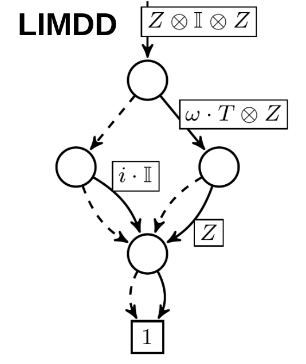
\includegraphics[width=3cm]{limdd}

\end{frame}








\section{Conclusion}

\begin{refsection}
\begin{frame}{Takeaways and Thank Yous}

\vspace{-1em}

\begin{itemize}
	\item \#SAT solvers effectively tackle quantum compilation problems
%	\item Better data structures yield better circuit simulation, equivalence checks \& synthesis
	\item \limdd unites the strengths of decision diagrams and the stabilizer formalism
	\item \limdd, MPS and RBM are incomparable in terms of succinctness
	\item Rapidity tells us that MPS and \limdd are never much slower than QMDD, ADD
\end{itemize}


\vspace{2em}

\pause

%\includegraphics[height=2cm]{graphics/thanos.jpg}
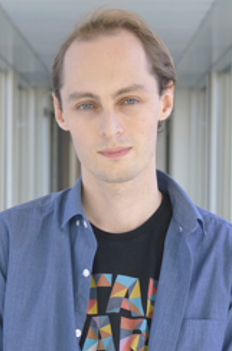
\includegraphics[height=2cm]{graphics/brand.png}
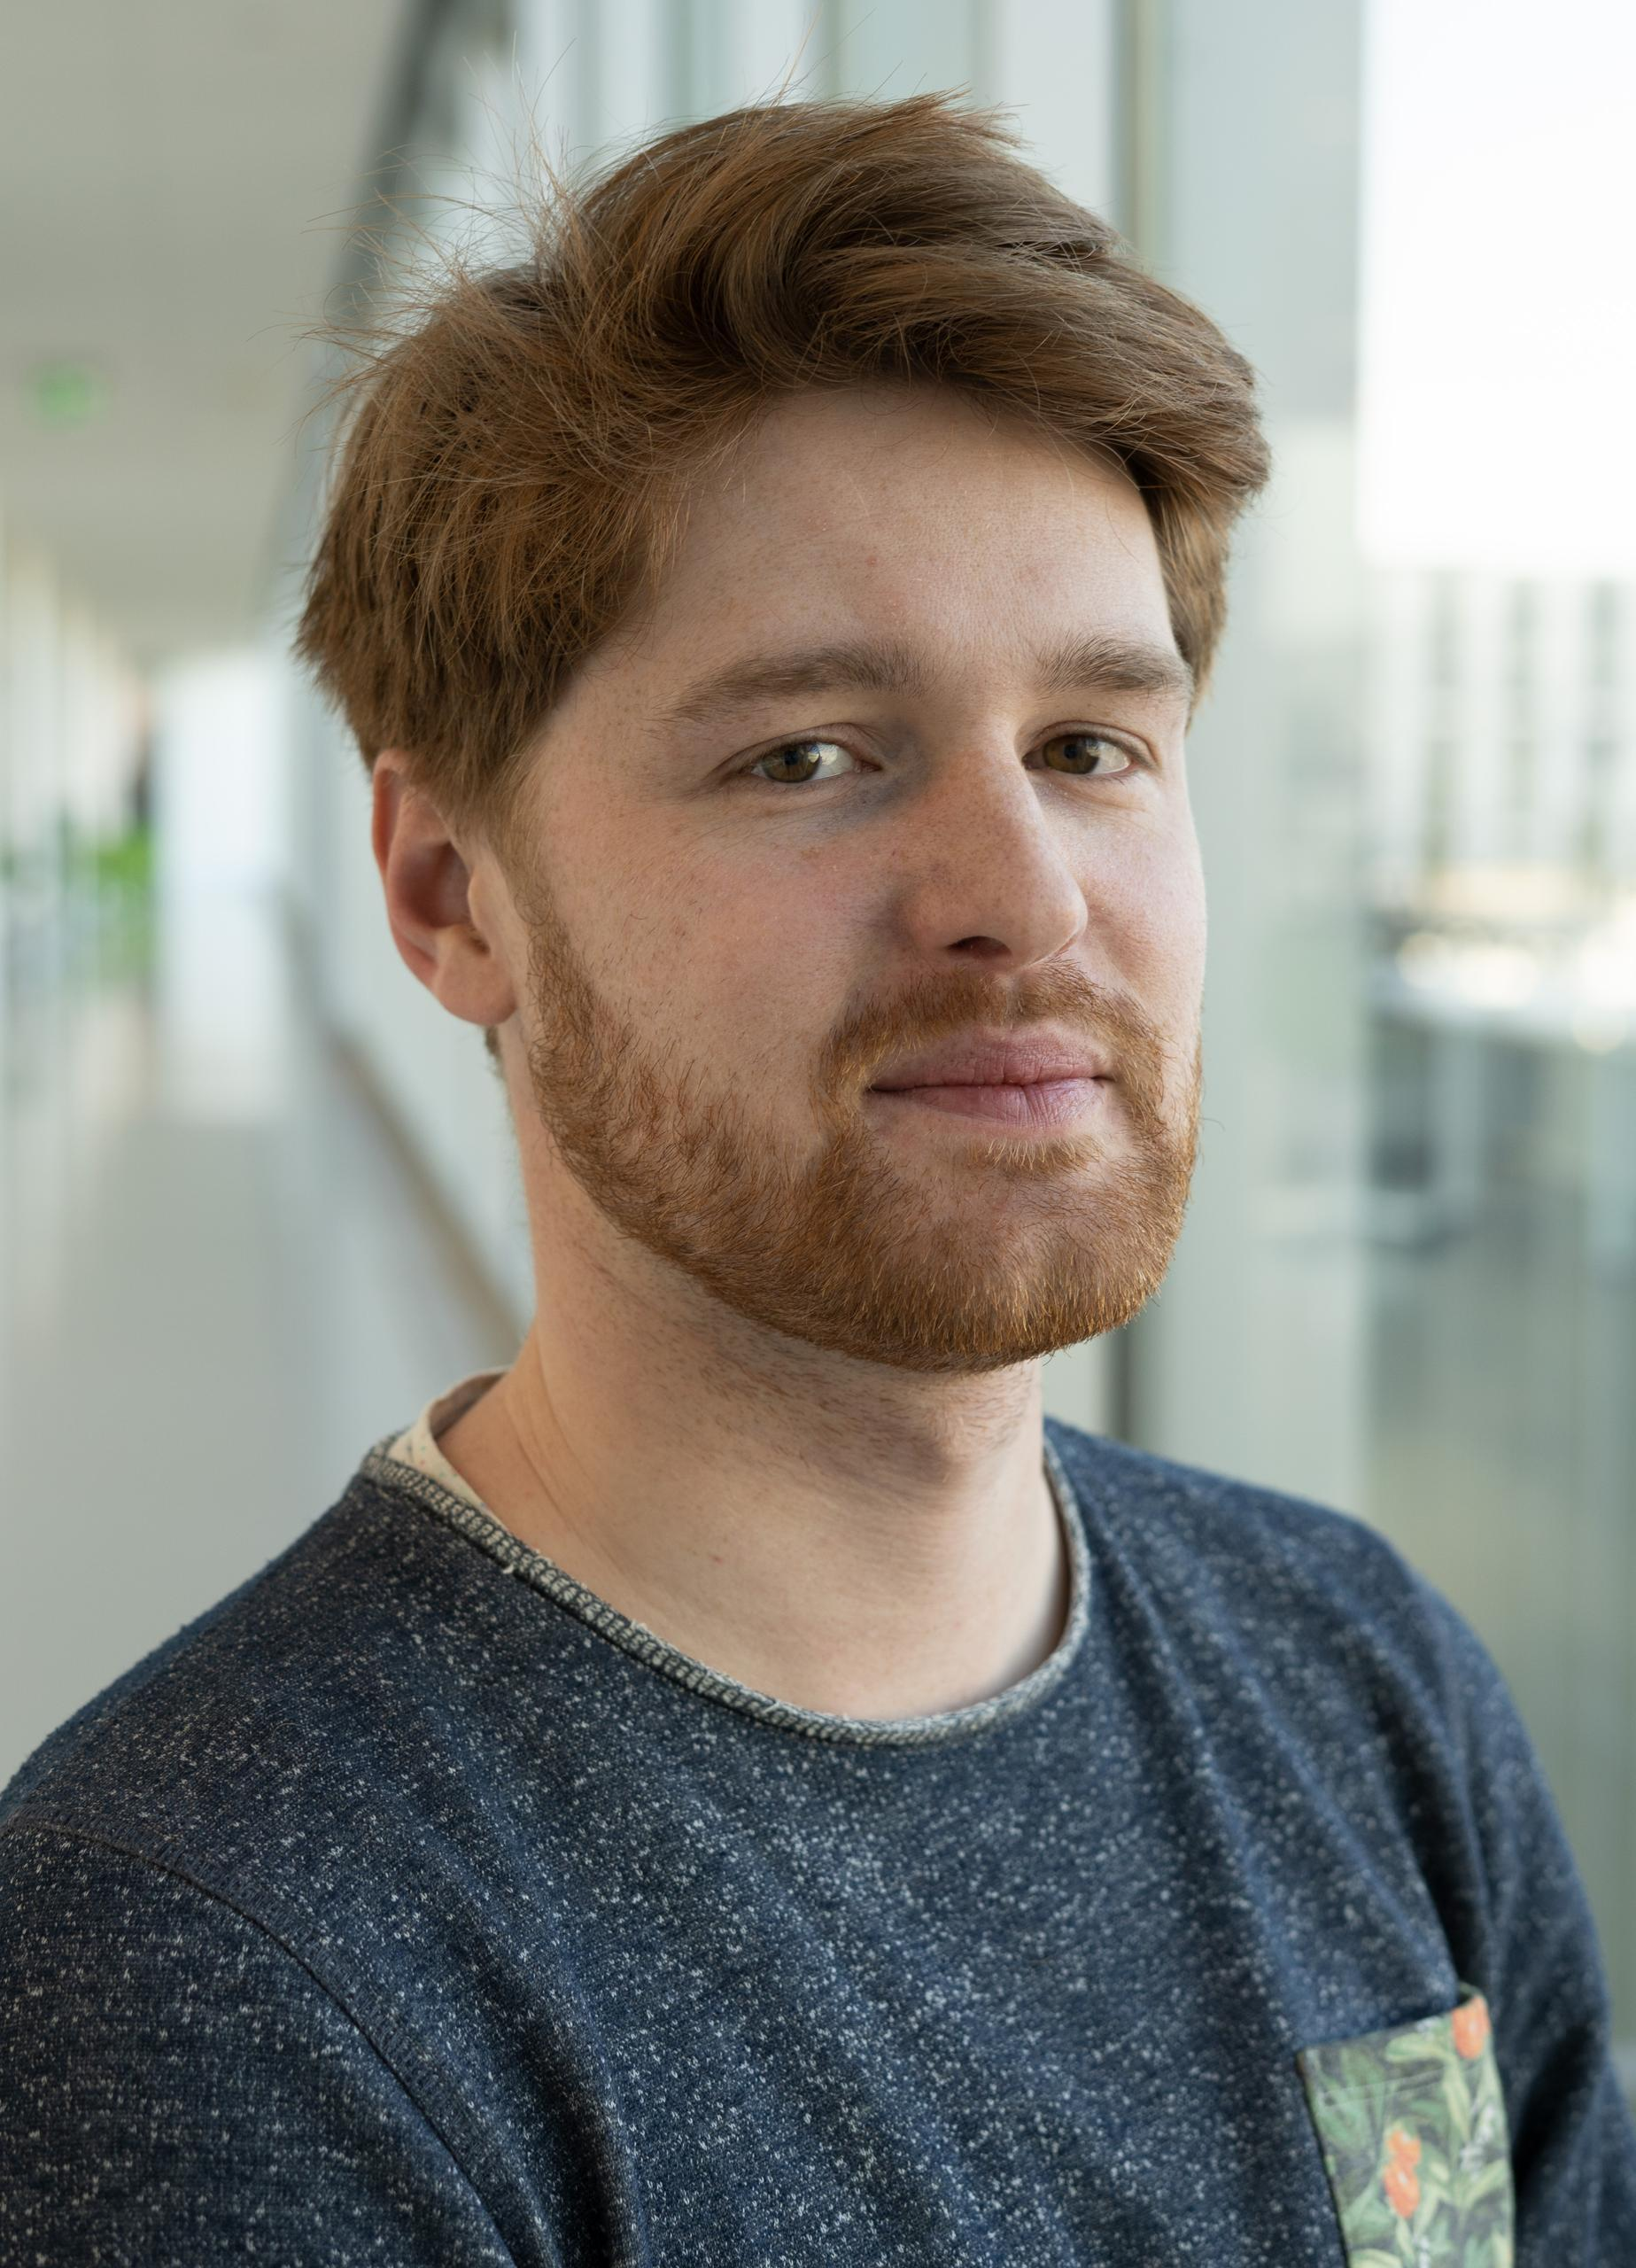
\includegraphics[height=2cm]{graphics/coopmans_tim}
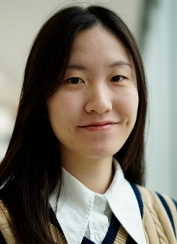
\includegraphics[height=2cm]{graphics/mei.png}
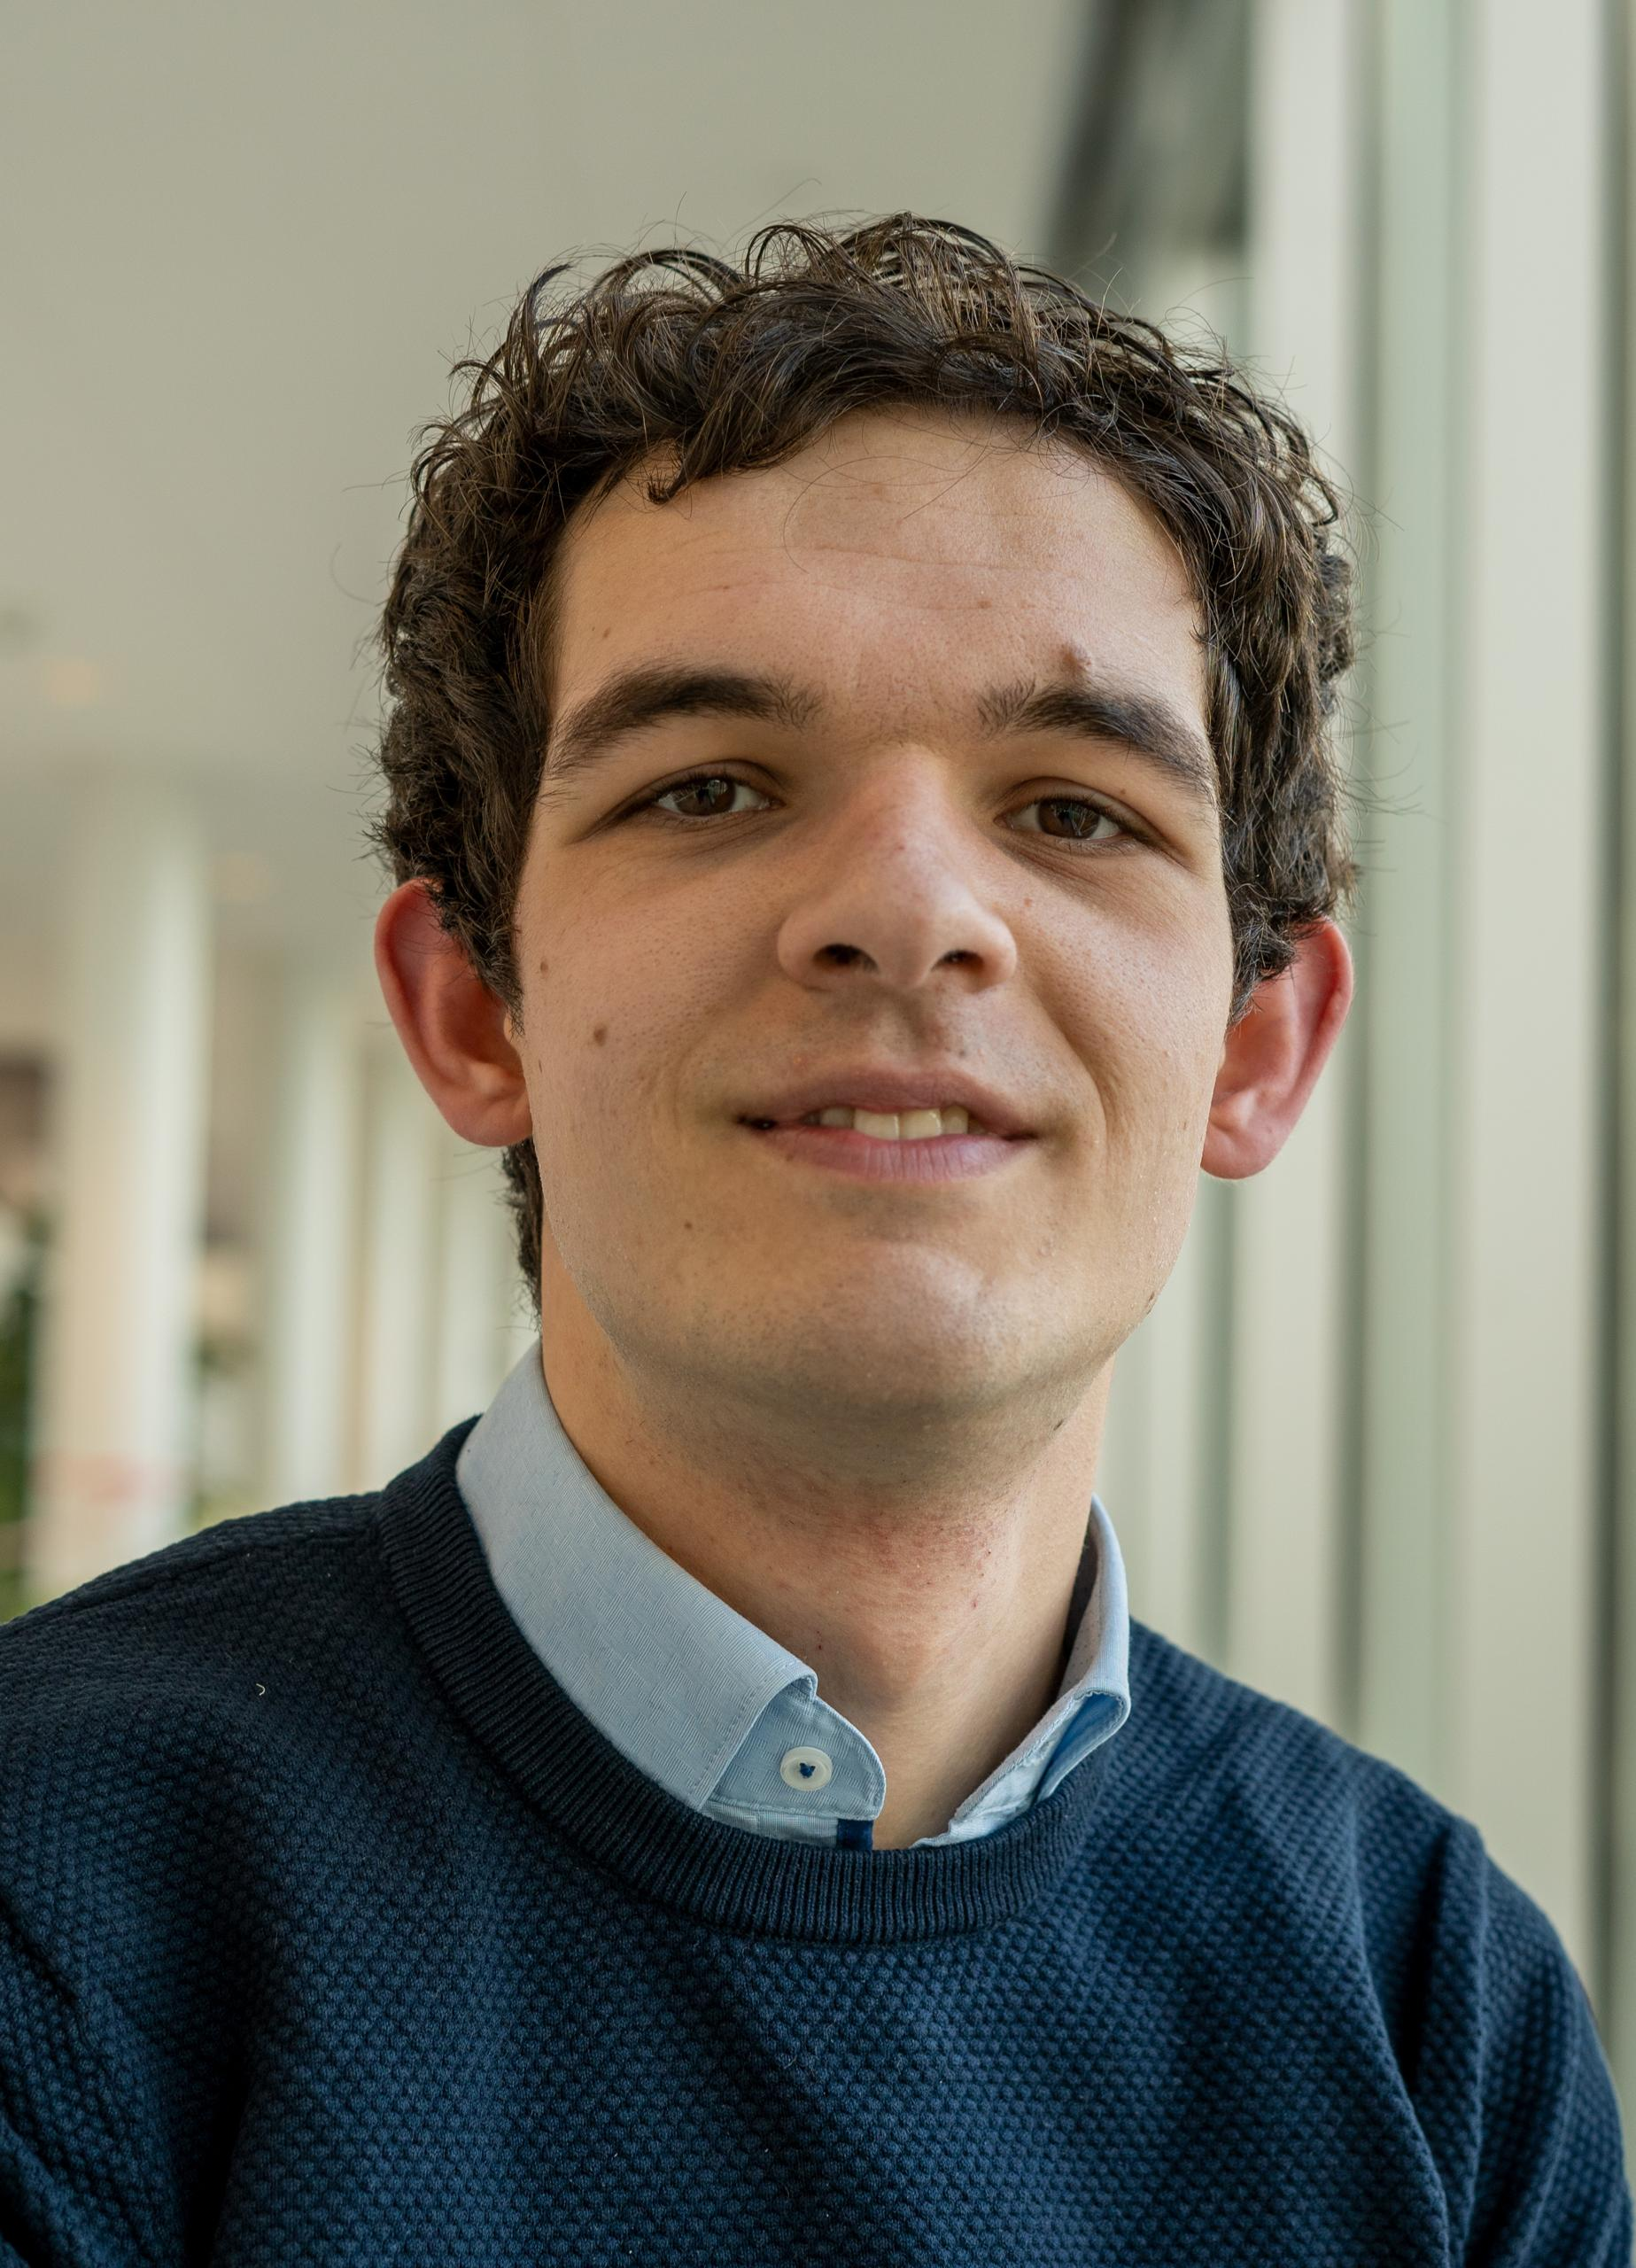
\includegraphics[height=2cm]{graphics/quist_arend-jan.jpg}

\includegraphics[height=2cm]{graphics/dimitrios}
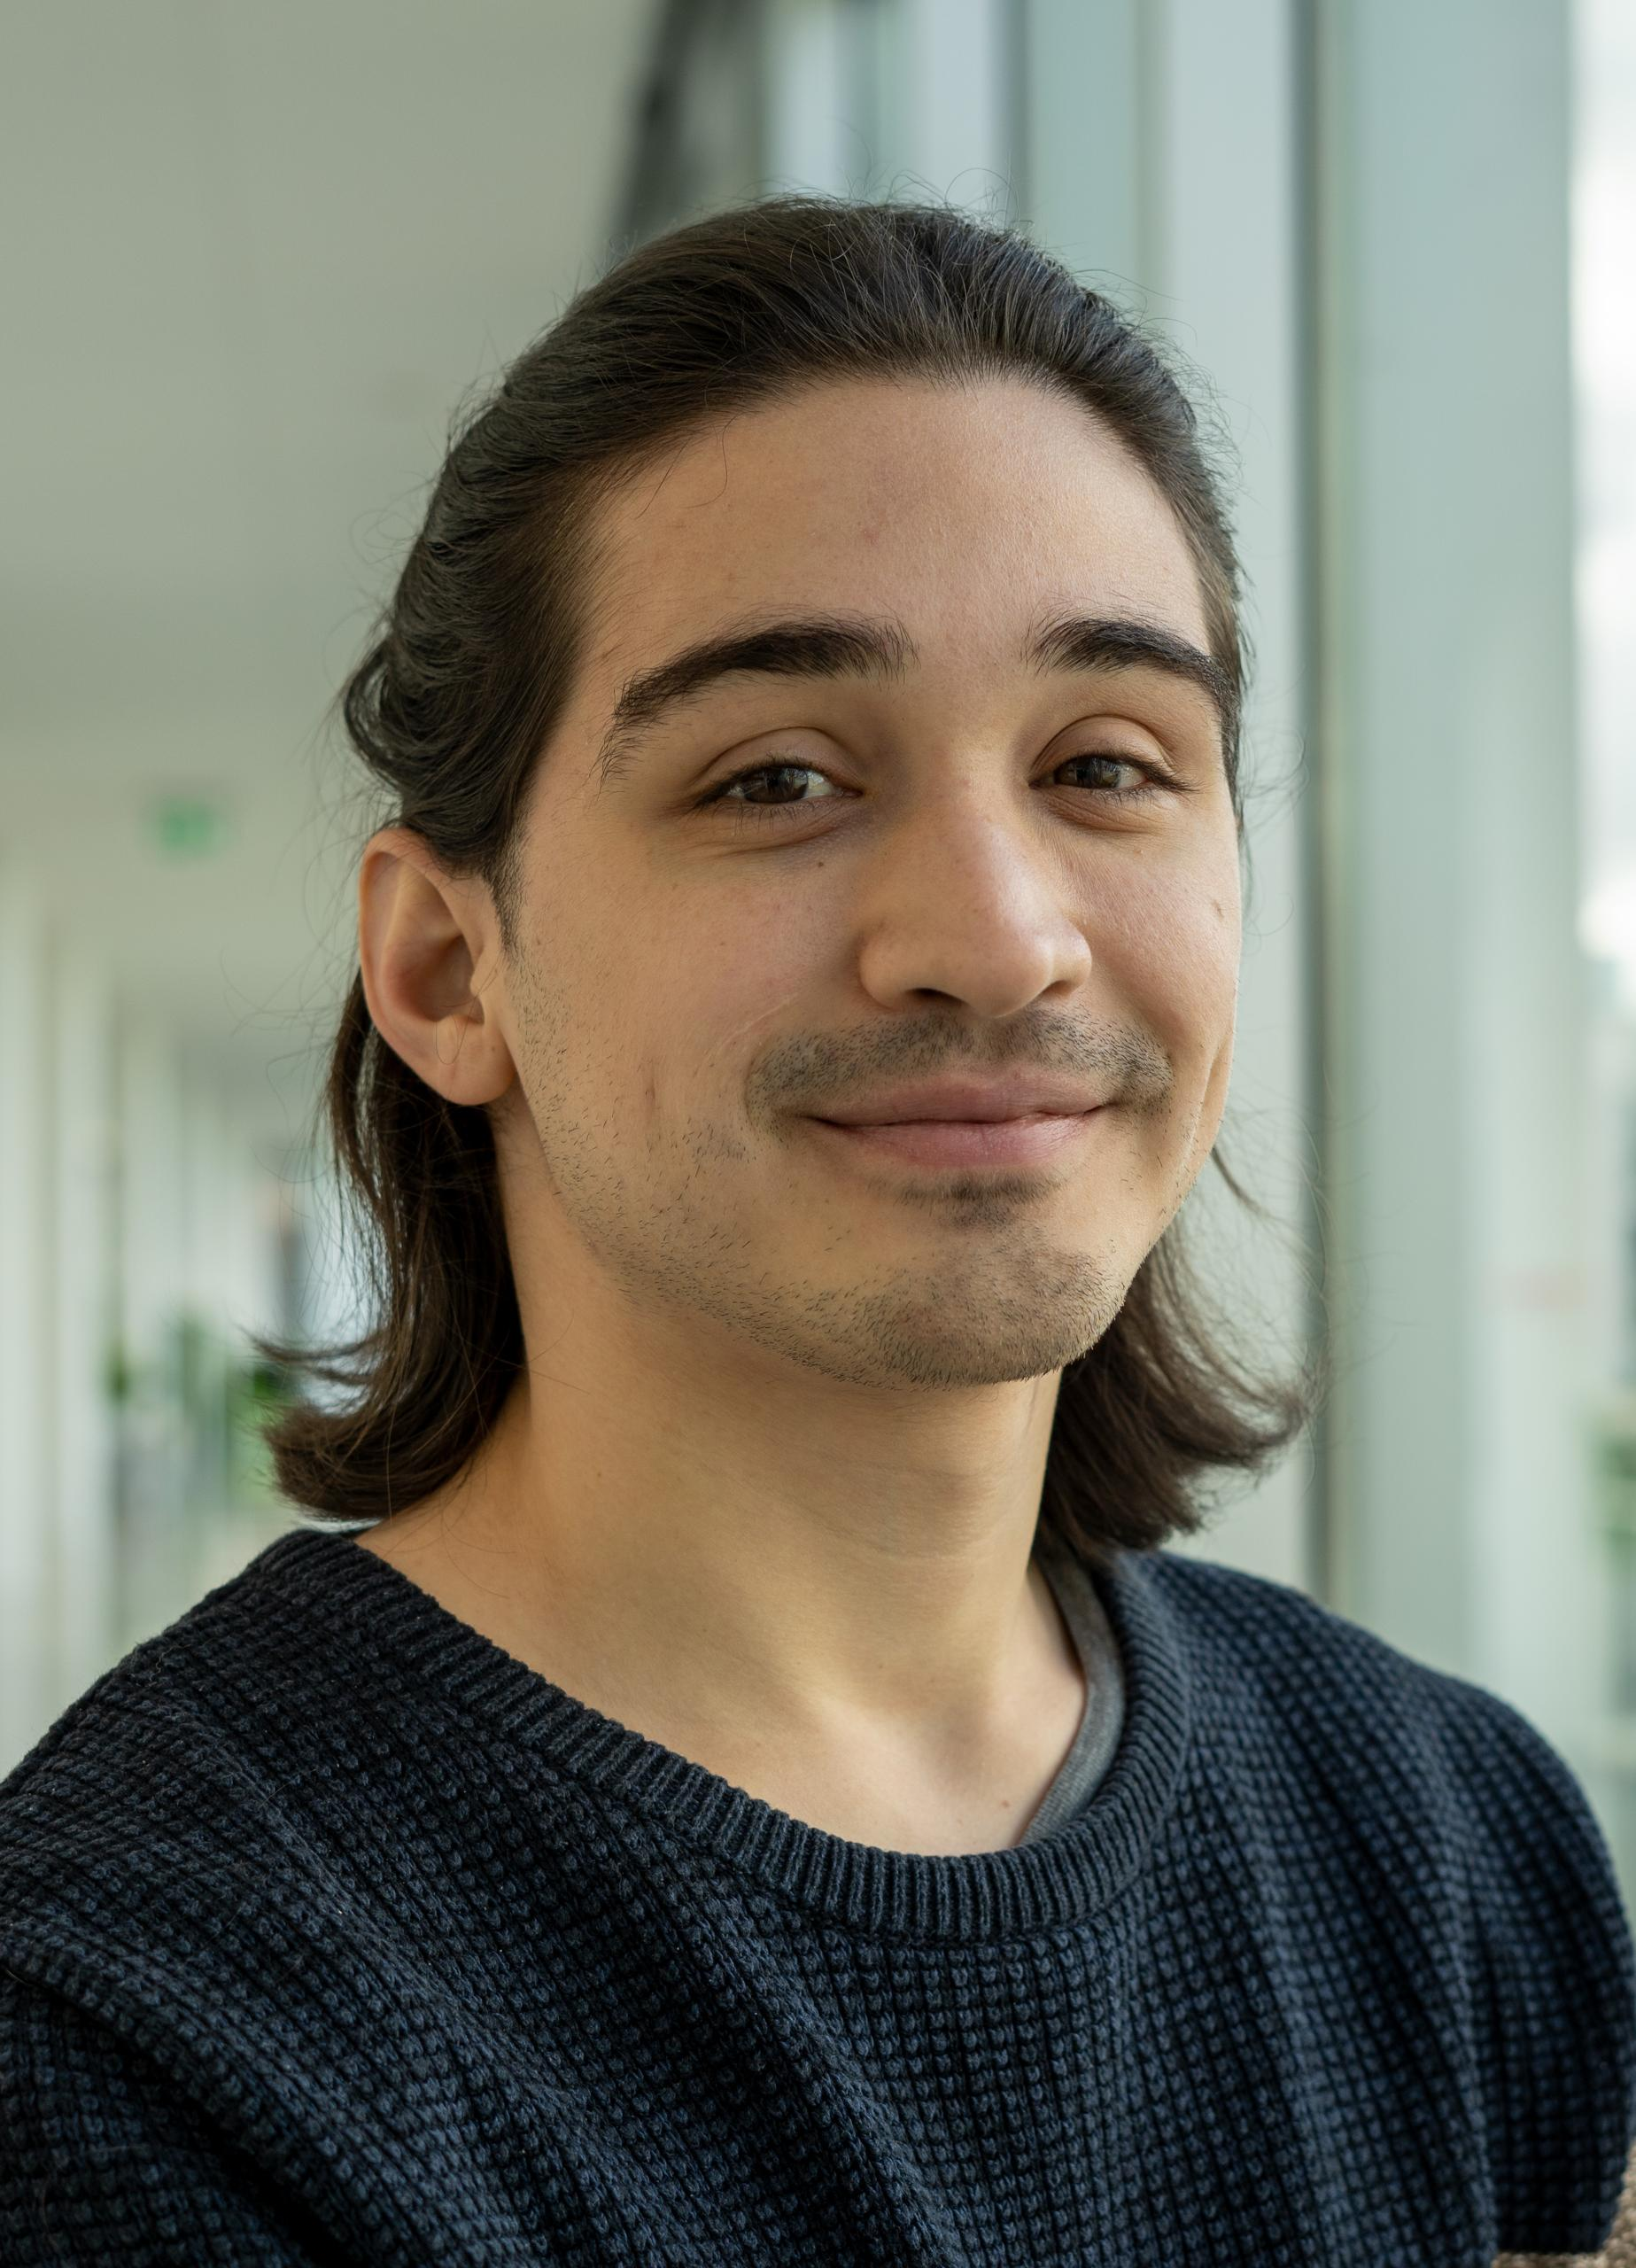
\includegraphics[height=2cm]{graphics/villoria_alejandro.jpg}
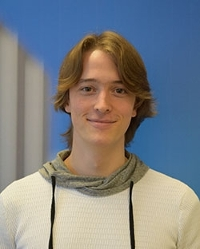
\includegraphics[height=2cm]{graphics/lieuwe.jpeg}
%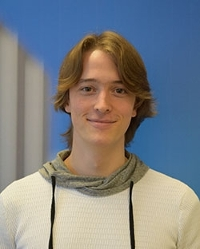
\includegraphics[width=2cm]{graphics/lieuwe}

\footnotesize
Sebastiaan Brand~~~~~~~~~~~~~~~~~~~
Jingyi Mei~~~~~~~~~~~~~~~~~~~~~~~~~~ 
Dimitrios Thanos~~~~~~~~~~~~~~~~~~~~
Lieuwe Vinkhuijzen

\vspace{-2ex}
~~~~~~~~~~~~~~~~~~
Tim Coopmans~~~~~~~~~~~~~~~~~~~~~
Arend-Jan Quist~~~~~~~~~~~~~~~~~~
Alejandro Villoria


\vspace{-1em}

\phantom{\cite{limdd,vinkhuijzen2024a,mei2024simulating,mei2024eq}}


%\vfill
%\centering
%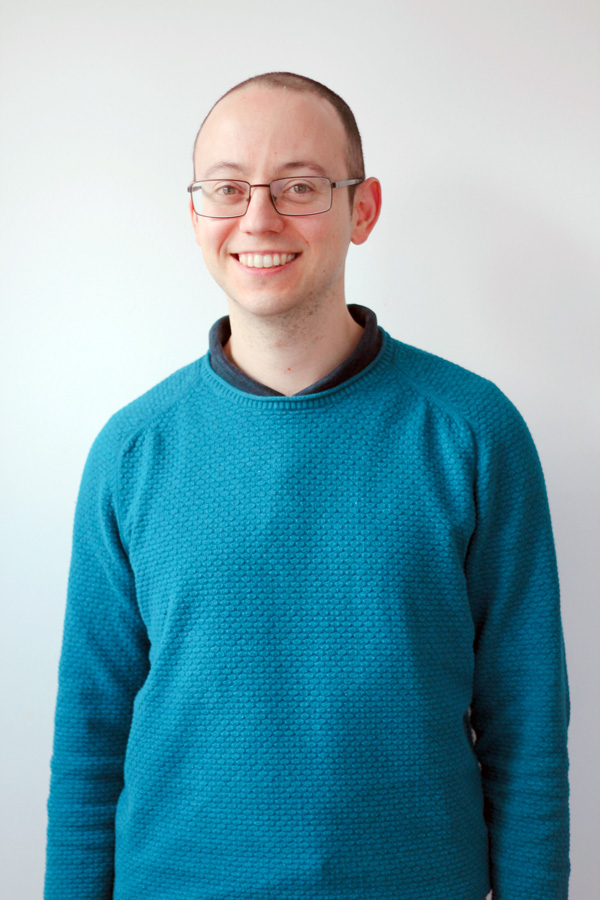
\includegraphics[height=2cm]{graphics/elkouss-david-20211227-torso_0}
%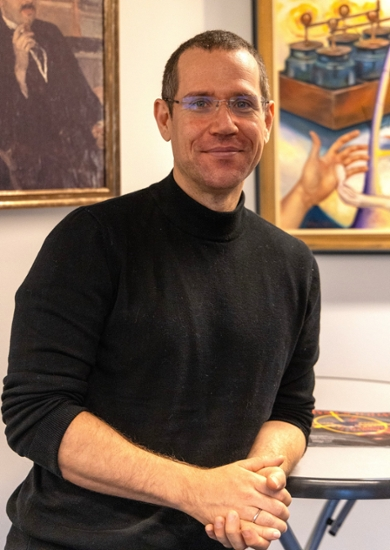
\includegraphics[height=2cm]{graphics/vedran-jobs}
%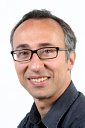
\includegraphics[height=2cm]{graphics/bonsangue}
%
%~~David Elkouss (Okinawa, Delft) ~~~
%Marcello Bonsangue (Leiden)

%\vspace{-2ex}
%Vedran Dunjko (Leiden)


\printbibliography[section=\therefsection]
\end{frame}
\end{refsection}




\appendix
\backupbegin
%\section{Quantum Computing 101}




\begin{frame}{Quantum States}
%	\framesubtitle{The proof uses \textit{reductio ad absurdum}.}



\begin{columns}%[onlywidth,T]
	\begin{column}{.4\textwidth}
\[
\def\arraystretch{1.15}
\underbrace{\scalebox{2}{$\ket{\phi}$}}_{n \text{ qubit state}}
~~~~~=~
\left.
\begin{bmatrix*}[c]
    \frac{i+1}{\sqrt 6} \\ 0 \\ 0 \\ 0\\ \vdots \\0\\ \frac1{\sqrt 3} \\ 0 \\\frac1{\sqrt 3} 
\end{bmatrix*}
~~\right \}\text{$2^n$-sized vector}
\]  
	\end{column}
%\pause
	\begin{column}{.6\textwidth}
\vspace{3mm}\[
\def\arraystretch{1.2}
\scalebox{1.}{$\ket{00\dots01}$}
~=~
\begin{bmatrix*}[c]
    0 \\ 1 \\ 0 \\ 0\\ \vdots \\0\\ 0  \\ 0 \\ 0 
\end{bmatrix*}
\begin{matrix*}[c]
	{\text{$\leftarrow$ index \scriptsize 00\dots00 }} \\ 
	{\text{$\leftarrow$ index \scriptsize 00\dots01 }} \\ \\ \\ \\ \\ \\ \\  
	{\text{$\leftarrow$ index \scriptsize 11\dots10 }} \\  
	{\text{$\leftarrow$ index \scriptsize 11\dots11 }} \\ 
\end{matrix*}
\]  	
	\end{column}
\end{columns}
\pause
\begin{columns}%[onlywidth,T]
	\begin{column}{1\textwidth}
\[
\def\arraystretch{.9}
\scalebox{2}{$\ket{\phi}^\dagger$}
~~=~~
\scalebox{2}{$\bra{\phi}$}
~~=~~
\underbrace{
\begin{bmatrix*}[c]
    \frac{\alert -i+1}{\sqrt 6} ,& 0 ,& 0 ,& 0,& \dots ,&0,&  \frac1{\sqrt 3} ,& 0 ,& 0 ,& \frac1{\sqrt 3} 
\end{bmatrix*}
}_{\text{$2^n$-sized vector (\alert{conjugated} and transposed)}}
\]  
	\end{column}
\end{columns}

\pause

  	\begin{block}{Normalization}
		For $\ket{\phi} =  \begin{bmatrix}\alpha_1, \alpha_2, \dots, \alpha_{n-1}, \alpha_n\end{bmatrix}^T$, we have that $\sum |\alpha_i| = 1$.
		
		~\\
		Or alternatively: $\braket{b|\phi} = \bra{b}\cdot \ket{\phi} = 1$.
  	\end{block}


%  	\begin{block}{Alternative interpretation as pseudo-Boolean function}
%%  		\begin{itemize}
%%  			\item 
%  			A pseudo-Boolean function $f_\phi \colon \set{0,1}^n \to \complex$ such that $f(b) = \braket{b|\phi} = \bra{b}\cdot \ket{\phi}$.
%%  			\\
%%  			~\\
%%  			Here $\bra{b}$ for $b \in \set{0,1}^n$ is a (conjugated) computational basis state, e.g.: $\bra{01} = \begin{bmatrix}0, 0, 0, 0\end{bmatrix}$.
%%  		\end{itemize}
%  	\end{block}


\end{frame}



\begin{frame}{Reversible computing (still classical)}

%\scriptsize
\centering

A circuit computing $(a\land b) \lor c$:

\scalebox{.7}{
\begin{circuitikz}
\draw
(0,2) node[and port] (myand) {\hspace{-1ex}$\land$}
(2,1) node[or port] (myor) {\hspace{-1ex}$\lor$}
(myand.in 1) node[anchor=east] {$a$}
(myand.in 2) node[anchor=east] (bnode) {$b$}
(myand.out) -| node[above]{$x$} (myor.in 1)
node[below=.638cm of bnode] (cnode) {$c$}
(cnode) -|  (myor.in 2)
(myor.out) node[anchor=west] {$y$}
;
\end{circuitikz}
}

How to compute $a,b,c$ given $y$?


\pause

\begin{minipage}{6cm}
\Qcircuit @C=2.em @R=.2em @!R  {
& \lstick{a} & \ctrl{1} & \qw  & \qw      & \qw \\
& \lstick{b} & \ctrl{2} & \qw  & \qw		 & \qw \\
& \lstick{c} & \qw      & \qw  & \ctrl{1} & \qw &\\
& \lstick{x = x_0} & \gate{\land}& \qw&\ctrl{1} & \qw &\rstick{ a\land b}   \\
& \lstick{y = y_0} & \qw      & \qw  & \gate{\lor}&\qw &\rstick{  x\lor c} \\
}
\end{minipage}

\pause
But how to revert the value of $x_0$ and $y_0$?

\pause

\begin{minipage}{6cm}
\Qcircuit @C=2.em @R=.5em @!R  {
& \lstick{a} & \multigate{1}{\land} & \qw  & \qw      & \qw \\
& \lstick{b} & \ghost{\land}  & \qw  & \qw		 & \qw \\
& \lstick{c} & \qw  & \qw  & \multigate{1}{\lor} & \qw &\\
& \lstick{x\alert{=0}} & \targ \qwx[-2] & \qw&\ghost{\land}  & \qw     &\rstick{ x \oplus (a\land b)}  \\
& \lstick{y\alert{=0}} & \qw      & \qw  & \targ \qwx[-1] &\qw &\rstick{y \oplus (x\lor c)} \\
}
\end{minipage}

~\\
\alert{XOR ($\oplus$) is invertible on one input:
$(x\oplus a)\oplus a = x\oplus (a\oplus a) = x$}


\end{frame}



\begin{frame}{Uncomputing reversible computations}

%\scriptsize

\vfill


For any function $f\colon \bool^k \to \bool$, the gate~~~
\begin{minipage}{1cm}
\Qcircuit @C=1em @R=.7em {
&{/}\qw 	& \gate{f} 		& \qw & \qw\\
&\qw  	& \targ\qwx[-1]	& \qw & \qw \\
}
\end{minipage}
~~~is its own inverse!

\pause
\vfill

\hspace{2.5cm}\begin{minipage}{8cm}
\only<1>{
\Qcircuit @C=2.em @R=.5em @!R  {
 \lstick{a} & \multigate{1}{\land} 	& \qw  		& \qw
 			\\
 \lstick{b} & \ghost{\land}        	& \qw		& \qw 
 			\\
 \lstick{c} & \qw    				& \multigate{1}{\lor} & \qw 
 			\\
 \lstick{x{=0}} &\targ \qwx[-2]	&\ghost{\land} & \qw 			
 			&\rstick{ x \oplus ( a\land b)}  \\
 \lstick{o{=0}} & \qw     & \targ \qwx[-1] &\qw 				
 			&\rstick{ o \oplus ( x\lor c)} \\
}
}
\only<+>{
\Qcircuit @C=2.em @R=.5em @!R  {
 \lstick{a} & \multigate{1}{\land} 	& \qw  		& \qw			& \qw & \qw
 			\\
 \lstick{b} & \ghost{\land}        	& \qw		& \qw 			& \qw & \qw
 			\\
 \lstick{c} & \qw    				& \multigate{1}{\lor} & \qw & \multigate{1}{\lor}& \qw
 			\\
 \lstick{x{=0}} &\targ \qwx[-2]	&\ghost{\land} & \qw 			& \ghost{\land}& \qw 
 			&\rstick{ x\oplus ( a\land b)}  \\
 \lstick{o{=0}} & \qw     & \targ \qwx[-1] &\qw 				& \targ \qwx[-1]& \qw
 			&\rstick{  o \oplus ( x\lor c) \oplus ( x\lor c) \alert{= 0}  } \\
}
}
\only<+->{
\Qcircuit @C=2.em @R=.5em @!R  {
 \lstick{a} & \multigate{1}{\land} 	& \qw  		& \qw			& \qw 				& \multigate{1}{\land}& \qw
 			\\
 \lstick{b} & \ghost{\land}        	& \qw		& \qw 			& \qw 				& \ghost{\land} & \qw
 			\\
 \lstick{c} & \qw    				& \multigate{1}{\lor} & \qw & \multigate{1}{\lor}& \qw& \qw
 			\\
 \lstick{x{=0}} &\targ \qwx[-2]	&\ghost{\land} & \qw 			& \ghost{\land}		& \targ \qwx[-2]& \qw
 			&\rstick{  \alert{0} }  \\
 \lstick{o{=0}} & \qw     & \targ \qwx[-1] &\qw 				& \targ \qwx[-1]	& \qw& \qw
 			&\rstick{ \alert{0}} \\
}
\vfill 

~\\
\hspace{-1cm}\alert{To uncomputate, we invert the gate order!}
}
\end{minipage}

\vfill 

\centering

\onslide<+->{
\begin{minipage}{6cm}
\Qcircuit @C=2.em @R=.5em @!R  {
 \lstick{a} & \multigate{1}{\land} 	& \qw  		& \qw						& \multigate{1}{\land}& \qw
 			\\
 \lstick{b} & \ghost{\land}        	& \qw		& \qw 							& \ghost{\land} & \qw
 			\\
 \lstick{c} & \qw    				& \multigate{1}{\lor} & \qw & \qw& \qw
 			\\
 \lstick{x{=0}} &\targ \qwx[-2]	&\ghost{\land} & \qw 				& \targ \qwx[-2]& \qw
 			&\rstick{  {0} }  \\
 \lstick{o{=0}} & \qw     & \targ \qwx[-1] &\qw 					& \qw& \qw
 			&\rstick{ {ab \lor c} \leftarrow \text{cannot uncompute}} \\
}
\end{minipage}
}

\onslide<+->{
\alert{Now to uncompute ${ab \lor c}$, we need to first recompute ${ab}$ }
}


\vfill

\pause
	\textsc{\footnotesize [Landauer (1961)]~~~~~~~~~~~~~~~[Bennett (1973) Logical reversibility of computing]}

\end{frame}



\begin{frame}{Reversible space and time}
	
	
	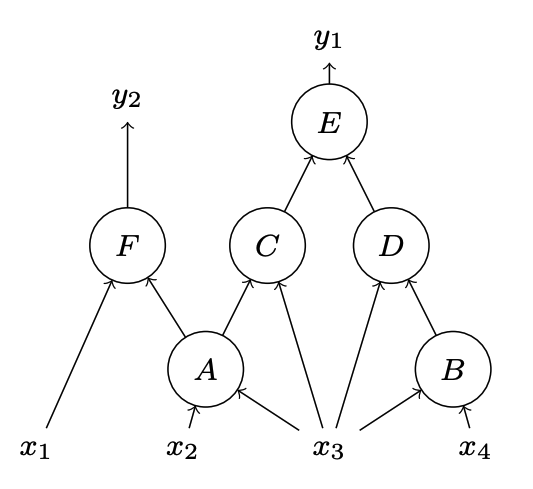
\includegraphics[height=3.cm]{ms1}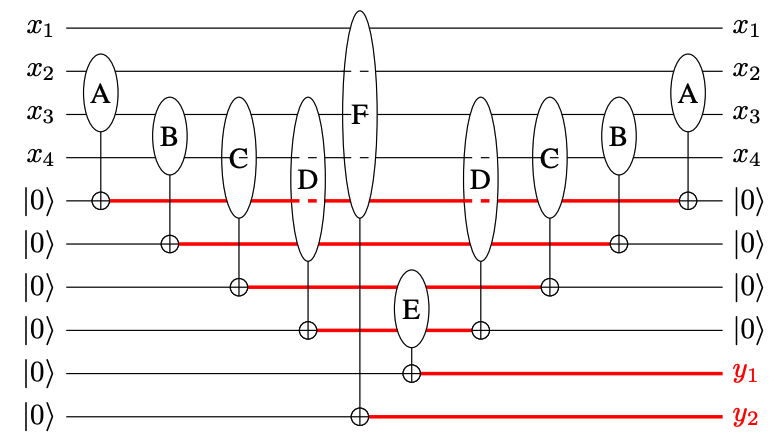
\includegraphics[height=3.5cm]{ms2}
	\raisebox{1.7cm}{\begin{minipage}{1cm}
			$\left . \crule[white]{0cm}{2.5em} \right \}$inputs  \\
			$\left . \crule[white]{0cm}{2.5em} \right \}$ancillas\\
			$\left . \crule[white]{0cm}{1em} \right \}$outputs
			\end{minipage}
	}

\centering 
\onslide<2->{
Do we need one bit per gate?~~~~~~~ Expensive: Space = Time.
}

\onslide<3->{
	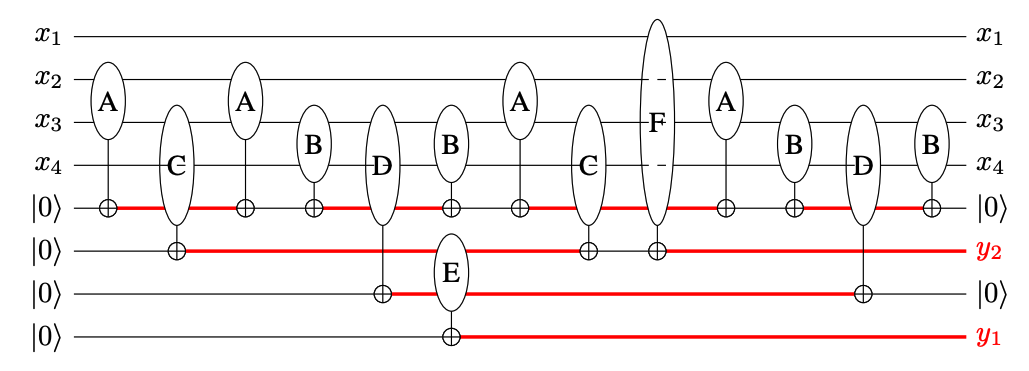
\includegraphics[height=3.cm]{ms3}
}

	\vspace{-1em}
	\textsc{\footnotesize [Meuli et al. (2019) Reversible Pebbling Game for Quantum Memory Management]}

\end{frame}



\begin{frame}{Reversible Circuit Evaluation with Matrices}


\begin{exampleblock}{One-qubit case}

\begin{columns}
\begin{column}{.2\textwidth}
A one bit circuit:\\\vspace{2ex}
\hspace{1em}\Qcircuit @C=1em @R=.7em {
\lstick 0  	& \gate{\neg} 		& \qw & \rstick 1 \\
%\lstick 0   	& \targ\qwx[-1]	& \qw & \qw \\
}
\end{column}
%\begin{column}{.15\textwidth}
%	\tab{0 \\ 1 } \mat{a\\b}
%\end{column}
\begin{column}{.3\textwidth}
\pause
.. with \textit{vectors as states}:\\\vspace{2ex}
~\phantom{ZZZZZ}\Qcircuit @C=1em @R=.7em {
\lstick{\mat{1\\0}}  	& \gate{\neg} 		& \qw & \rstick{\mat{0\\1}} \\
%\lstick 0   	& \targ\qwx[-1]	& \qw & \qw \\
}
\end{column}
\begin{column}{.3\textwidth}
.. not ($\neg$) is a matrix:\\\vspace{1ex}
$X = \mat{0 & 1\\ 1 & 0}$
\end{column}
\end{columns}


\vspace{2em}

\pause
\begin{columns}
\begin{column}{.45\textwidth}
So evaluation becomes matrix-vector multiplication:\\
~
\end{column}
\begin{column}{.45\textwidth}
$\underbrace{\mat{0& 1\\ 1 & 0}}_{X}\cdot \mat{1\\ 0} =  \mat{0\\ 1}$
\end{column}
%\begin{column}{.25\textwidth}
%$\underbrace{\mat{1& 1\\ 1 & 1}}_{?}\cdot \mat{1\\ 0} =  \mat{1\\ 1}$
%\end{column}
\end{columns}



\vspace{1ex}
\vspace{1ex}
\vspace{1ex}
\pause

\alert{We read circuits from left to right, but the linear algebra works the other way around!}

\begin{align*}
\hspace{1em}\Qcircuit @C=1em @R=.7em {
\lstick{\mat{1\\0}}  	& \gate{A} & \gate{B} & \gate{C} 		& \qw & 
%\lstick 0   	& \targ\qwx[-1]	& \qw & \qw \\
}
=   C\cdot B \cdot A \cdot \mat{1\\0}
\end{align*}


\vspace{1ex}
\end{exampleblock}

	
\end{frame}




\begin{frame}{Reversible Circuit Evaluation with Matrices}

\begin{exampleblock}{Multi-qubit case}

\begin{columns}
\begin{column}{.24\textwidth}
\hspace{1em}Three-bit circuit:\\\vspace{2ex}
\hspace{2.5em}\Qcircuit @C=1em @R=.7em {
\lstick 1  	& \multigate{1}{\land}	& \qw & \rstick 1 \\
\lstick 1  	& \ghost{\land}			& \qw & \rstick 1 \\
\lstick 0   & \targ\qwx[-1]			& \qw & \rstick 1 \\
}
\end{column}
\begin{column}{.34\textwidth}
States become vectors..\\\vspace{1ex}
{$ \ket{110} = \smat{0 \\ 0 \\ 0 \\ 0 \\ 0 \\ 0 \\ 1 \\ 0 }\ket{111} = \smat{0 \\ 0 \\ 0 \\ 0 \\ 0 \\ 0 \\ 0 \\ 1 }$}
\end{column}
\begin{column}{.4\textwidth}
.. Tofolli gate becomes a matrix:\\\vspace{1ex}
$CCX = \smat{1 & 0 & 0 & 0 & 0 & 0 & 0 & 0 \\
			0 & 1 & 0 & 0 & 0 & 0 & 0 & 0 \\
			0 & 0 & 1 & 0 & 0 & 0 & 0 & 0 \\
			0 & 0 & 0 & 1 & 0 & 0 & 0 & 0 \\
			0 & 0 & 0 & 0 & 1 & 0 & 0 & 0 \\
			0 & 0 & 0 & 0 & 0 & 1 & 0 & 0 \\
			0 & 0 & 0 & 0 & 0 & 0 & \alert 0 & \alert 1 \\
			0 & 0 & 0 & 0 & 0 & 0 & \alert 1 & \alert 0 \\}$
\end{column}
\end{columns}


\vspace{2em}

\pause
\begin{columns}
\begin{column}{.2\textwidth}
As matrix-vector multiplication:\\
~
\end{column}
\begin{column}{.7\textwidth}
$CCX \cdot \ket{110} = \smat{1 & 0 & 0 & 0 & 0 & 0 & 0 & 0 \\
			0 & 1 & 0 & 0 & 0 & 0 & 0 & 0 \\
			0 & 0 & 1 & 0 & 0 & 0 & 0 & 0 \\
			0 & 0 & 0 & 1 & 0 & 0 & 0 & 0 \\
			0 & 0 & 0 & 0 & 1 & 0 & 0 & 0 \\
			0 & 0 & 0 & 0 & 0 & 1 & 0 & 0 \\
			0 & 0 & 0 & 0 & 0 & 0 & \alert 0 & \alert 1 \\
			0 & 0 & 0 & 0 & 0 & 0 & \alert 1 & \alert 0 \\} \cdot   \smat{0 \\ 0 \\ 0 \\ 0 \\ 0 \\ 0 \\ 1 \\ 0 } =  \smat{0 \\ 0 \\ 0 \\ 0 \\ 0 \\ 0 \\ 0 \\ 1} =  \ket{111}$
\end{column}
\end{columns}


\vspace{1ex}
\end{exampleblock}

\pause
\centering
\alert{Overkill to compute with exponentially sized vectors?}
	
\end{frame}




\begin{frame}{Superpositions}

\begin{exampleblock}{Adding superpositions}
\begin{columns}
\begin{column}{.25\textwidth}
A one bit circuit:\\\vspace{1ex}
\hspace{1em}\Qcircuit @C=1em @R=.7em {
\lstick 0  	& \gate{X} 		& \qw & \rstick 1 \\
%\lstick 0   	& \targ\qwx[-1]	& \qw & \qw \\
}
\end{column}
%\begin{column}{.15\textwidth}
%	\tab{0 \\ 1 } \mat{a\\b}
%\end{column}
\begin{column}{.3\textwidth}
\pause
 .. a `normal' operation:\\\vspace{1ex}
\hspace{1em}\Qcircuit @C=1em @R=.7em {
\lstick{\mat{1\\0}}  	& \gate{X} 		& \qw & \rstick{\mat{0\\1}} \\
%\lstick 0   	& \targ\qwx[-1]	& \qw & \qw \\
}

\end{column}
\begin{column}{.25\textwidth}
\pause
 .. superposition op.:\\\vspace{1ex}
\hspace{1em}
\Qcircuit @C=1em @R=.7em {
\lstick{\mat{1\\0}} 	& \gate{?} 		& \qw & \rstick{\mat{1\\1}} \\
%\lstick 0   	& \targ\qwx[-1]	& \qw & \qw \\
}
\end{column}
\end{columns}

\vspace{2em}

\pause
\begin{columns}
\begin{column}{.2\textwidth}
In linear algebra:\\
~
\end{column}
\begin{column}{.25\textwidth}
$\underbrace{\mat{0& 1\\ 1 & 0}}_{X}\cdot \mat{1\\ 0} =  \mat{0\\ 1}$
\end{column}
\begin{column}{.25\textwidth}
$\underbrace{\mat{1& 1\\ 1 & 1}}_{?}\cdot \mat{1\\ 0} =  \mat{1\\ 1}$
\end{column}
\end{columns}



\vspace{1ex}
\vspace{1ex}
\vspace{1ex}

\vspace{1ex}
\end{exampleblock}


\pause
\begin{alertblock}{Two problems}
\begin{enumerate}
	\item How to make this \alert{reversible}? We have:
$\mat{1& 1\\ 1 & 1}\cdot \alert{\mat{1\\ 0}} =  \mat{1& 1\\ 1 & 1}\cdot 
   \alert{\mat{0\\ 1}} =  \mat{1\\ 1}$
\pause
	\item What does the state \mat{1\\1} mean? Non-determinism? Parallelism? Probability?
\end{enumerate}
\end{alertblock}

\end{frame}




\begin{frame}{Superpositions and reversibility}

\begin{exampleblock}{Making superpositions reversible with a \alert{Hadamard gate}}


Define $\alert H = \nicefrac1{\sqrt 2}  \mat{1& 1\\ 1 & -1}$.

\pause
Note that $H\cdot H = 
%		\nicefrac1{\sqrt 2}  \mat{1& 1\\ 1 & -1} \cdot
%		\nicefrac1{\sqrt 2}  \mat{1& 1\\ 1 & -1} =
		\nicefrac12 \mat{2& 0\\ 0 & 2} = \mat{1& 0\\ 0 & 1} = \id$,
so we have \alert{reversibility:}
~\\

\begin{align*}
\Qcircuit @C=1em @R=.7em {
\lstick{\mat{a\\b}} 	& \gate{H} 		& \gate{H} 	 & \qw & \rstick{\hspace{-1em} \mat{a\\b }} & \\
%\lstick 0   	& \targ\qwx[-1]	& \qw & \qw \\
} 
~~=~~
\Qcircuit @C=1em @R=.7em {
&&\lstick{\mat{a\\b}} 	& \gate{\id}	 & \qw & \rstick{\hspace{-1em} \mat{a\\b }} & \\
%\lstick 0   	& \targ\qwx[-1]	& \qw & \qw \\
}
~~=~~
\Qcircuit @C=1em @R=.7em {
&&\lstick{\mat{a\\b}} 	& \qw & \qw & \qw & \rstick{\hspace{-1em} \mat{a\\b }} \\
%\lstick 0   	& \targ\qwx[-1]	& \qw & \qw \\
}
\end{align*}

~\\
~\\

\pause

\vspace{2ex}
\begin{columns}
\begin{column}{.1\textwidth}
\end{column}
\begin{column}{.4\textwidth}
From `basis state' 0:\\\vspace{2ex}
\hspace{1em} \Qcircuit @C=1em @R=.7em {
\lstick{\mat{1\\0}} 	& \gate{H} 		& \qw & \rstick{\hspace{-1em} \frac1{\sqrt 2} \mat{1\\1}} \\
%\lstick 0   	& \targ\qwx[-1]	& \qw & \qw \\
}
\end{column}
\begin{column}{.4\textwidth}
From `basis state' 1:\\\vspace{2ex}
\hspace{1em}
\Qcircuit @C=1em @R=.7em {
\lstick{\mat{0\\1}} 	& \gate{H} 		& \qw & \rstick{\hspace{-1em}\frac1{\sqrt 2} \mat{1\\-1}} \\
%\lstick 0   	& \targ\qwx[-1]	& \qw & \qw \\
}
\end{column}
\end{columns}

\vspace{2em}

\pause
\begin{columns}
\begin{column}{.02\textwidth}
%In linear algebra:
\end{column}
\begin{column}{.4\textwidth}
$\frac1{\sqrt 2}\mat{1& 1\\ 1 & -1}\cdot \mat{1\\ 0} =  \frac1{\sqrt 2}\mat{1\\ 1}$
\end{column}
\begin{column}{.4\textwidth}
$\frac1{\sqrt 2}\mat{1& 1\\ 1 & -1}\cdot \mat{0\\ 1} = \frac1{\sqrt 2} \mat{1\\ -1}$
\end{column}
\end{columns}


\vspace{1.5em}

\vspace{1ex}
\end{exampleblock}


\end{frame}




\begin{frame}{Superpositions on the superbit plane}


\centering



%\begin{textblock}{6}(.5,.3)
%\only<2->{
	\begin{tikzpicture}[scale=1.9,cap=round,>=latex,font=\scriptsize]

        \draw[-] (1.5cm,0cm) -- (-1.5cm,0cm) node[left,fill=white]
        {\hphantom{$x \text{(basis state 0)} $}};

        % draw the coordinates
        \draw[->] (-1.5cm,0cm) -- (1.5cm,0cm) node[right,fill=white] {$x \text{(basis state 0)} $};
        \draw[->] (0cm,-1.5cm) -- (0cm,1.5cm) node[above,fill=white] {$y \text{(basis state 1)}$};



        % draw the unit circle
        \draw[thick] (0cm,0cm) circle(1cm);

        \foreach \x /\y  [evaluate=\y as \xtext using 180/\y]
          in {45} {
                % lines from center to point
                \draw[gray] (0cm,0cm) -- (\x:1cm);
                \draw[dotted] (0.71cm,0cm) -- node[left] {$\frac 1{\sqrt2}$} (\x:1cm);
                \draw[dotted] (0cm,0.71cm) -- node[above left] {$\frac 1{\sqrt2}$} (\x:1cm);
                % dots at each point
                \filldraw[black] (\x:1cm) circle(0.4pt);
                % draw each angle in degrees
                
                \draw (\x:1.45cm) node[fill=white] (a) {\mat{\nicefrac1{\sqrt2}\\ \nicefrac1{\sqrt2}} };
                
%              \draw[gray] (0cm,0cm) -- (-\x:1cm);              
%
%                \draw[dotted] (0.71cm,0cm) -- node[left] {$\frac 1{\sqrt2}$} (-\x:1cm);
%                \draw[dotted] (0cm,-0.71cm) -- node[above left] {$\frac 1{\sqrt2}$} (-\x:1cm);
%                
%%                \draw (\x:0.6cm) node[fill=white] {$\x^\circ$};
%                \draw (-\x:1.45cm) node[fill=white] (a) {\mat{\nicefrac1{\sqrt2}\\ -\nicefrac1{\sqrt2}} };
%%                \draw (\x:0.6cm) node[fill=white] {$\frac{\pi}{4}$};
        }

        \draw (-1.3cm,0cm) node[above=1pt] {$-1$}
              (1.25cm,0cm)  node[above=1pt] {$1$}
              (0.2cm,-1.25cm) node[] {$-1$}
              (0.2cm,1.25cm)  node[] {$1$};
              
%        \draw[bend left=20,->,dotted] (a)  node {} -- (5.2, 1.5);
    \end{tikzpicture}
%}
%\end{textblock}

\pause
\alert{Not the complex plane!}

\end{frame}



\begin{frame}{Superpositions and measurement}

\begin{exampleblock}{Making superpositions readable through \alert{measurement}}


\vspace{1ex}

\begin{columns}
\begin{column}{.1\textwidth}
\end{column}
%\begin{column}{.15\textwidth}
%	\tab{0 \\ 1 } \mat{a\\b}
%\end{column}
\begin{column}{.4\textwidth}
%From `basis state' 0:\\\vspace{2ex}
\hspace{1em} \Qcircuit @C=1em @R=.7em {
\lstick{\mat{1\\0}} 	& \qw 		& \meter &	\rstick{\tab{p(0) = 1 \\ p(1) = 0  }} \\
%\lstick 0   	& \targ\qwx[-1]	& \qw & \qw \\
}
\end{column}
\begin{column}{.4\textwidth}
%From `basis state' 1:\\\vspace{2ex}
\hspace{1em}
\Qcircuit @C=1em @R=.7em {
\lstick{\mat{0\\1}} 	& \qw		&  \meter &	\rstick{\tab{p(0) = 0\\ p(1) = 1  }}
%\lstick 0   	& \targ\qwx[-1]	& \qw & \qw \\
}
\end{column}
\end{columns}

\pause
\vspace{5ex}


\begin{columns}
\begin{column}{.1\textwidth}
\end{column}
%\begin{column}{.15\textwidth}
%	\tab{0 \\ 1 } \mat{a\\b}
%\end{column}
\begin{column}{.4\textwidth}
%From `basis state' 0:\\\vspace{2ex}
\hspace{1em} \Qcircuit @C=1em @R=.7em {
\lstick{\mat{1\\0}} 	& \gate{H} 		& \meter &	\rstick{\tab{p(0) = \nicefrac12 \\ p(1) = \nicefrac12  }} \\
%\lstick 0   	& \targ\qwx[-1]	& \qw & \qw \\
}
\end{column}
\begin{column}{.4\textwidth}
%From `basis state' 1:\\\vspace{2ex}
\hspace{1em}
\Qcircuit @C=1em @R=.7em {
\lstick{\mat{0\\1}} 	& \gate{H} 		&  \meter &	\rstick{\tab{p(0) = \nicefrac12 \\ p(1) = \nicefrac12  }}
%\lstick 0   	& \targ\qwx[-1]	& \qw & \qw \\
}
\end{column}
\end{columns}

\vspace{2em}

\pause

\begin{columns}
\begin{column}{.02\textwidth}
%In linear algebra:
\end{column}
\begin{column}{.4\textwidth}
$\frac1{\sqrt 2}\mat{1& 1\\ 1 & -1}\cdot \mat{1\\ 0} =  \mat{\nicefrac1{\sqrt2}\\ \nicefrac1{\sqrt2}}$
\end{column}
\begin{column}{.4\textwidth}
$\frac1{\sqrt 2}\mat{1& 1\\ 1 & -1}\cdot \mat{0\\ 1} =  \mat{\nicefrac1{\sqrt2}\\ \alert{-\nicefrac1{\sqrt2}}}$
\end{column}
\end{columns}

\pause

\centering
\vspace{1em}




\onslide<+->{}

In general, we have a state \mat{a \\ b}, which \ul{indirectly} represents a \alert{probability distribution:}

\vspace{1ex}
\begin{tabular}{c|c|c}
\bf Old state &	\bf Outcome 			& \onslide<+->{\bf New state} \\\hline
 \mat{a \\ b}  & 0 = \mat{1\\0}	with $p(0) = a^2$ & \onslide<.->{\mat{1\\0}}
  \rule{0cm}{.6cm}
  \\
 \mat{a \\ b}  & 1 = \mat{0\\1}	with $p(1) = b^2$ & \onslide<.->{\mat{0\\1}}	\rule{0cm}{.6cm}
\end{tabular}

\vspace{1ex}
\vspace{1ex}

\onslide<.->{
\alert{State collapses after measurement to measurement outcome!}
}

\vspace{1ex}
\end{exampleblock}


\end{frame}




\begin{frame}{Quantum State Representation with the
					\alert{Stabilizer Formalism}}

Pauli gates:~~~~ $I = \mat{1&0\\0&1},~~~~X = \mat{0&1\\1&0} ~~~~Y = \mat{0&-i\\i&0}~~~~Z = \mat{1&0\\0&-1}$

\begin{exampleblock}<2->{Stabilizing single-qubit states}

\begin{itemize}
	\item 
All single-qubit states $\ket{\phi}$ are stabilized by $\mathbb{I}$, because $I \cdot \ket{\phi}= \ket{\phi}$.

\item ~~$Z \cdot \ket{0} = \mat{1&0\\0&-1} \cdot \mat{1\\0} = \mat{1\\0} = \ket 0$
\item $-Z \cdot \ket{1} = \mat{-1&0\\0&1} \cdot \mat{0\\1} = \mat{0\\1} = \ket 1$
\pause
\item
\only<+>{ ~~$P \cdot \ket{+} = ~~P \cdot \mat{1\\1} = \mat{1\\1} = \ket +$ for which $P \in \set{\mathbb{I}, X, Y, Z}$?}
\pause
 ~~$X \cdot \ket{+} = ~~X \cdot \mat{1\\1} = \mat{1\\1} = \ket +$ 
\pause
\item
 $-X \cdot \ket{-} = ~~X \cdot \mat{1\\1} = \mat{1\\1} = \ket -$ 
\end{itemize}

\end{exampleblock}



\pause
\begin{exampleblock}{Two-qubit stabilizer states}

\begin{itemize}
	\item  $\ket{00}$ is stabilized by $I \otimes I, Z\otimes I, I\otimes Z$ and $Z\otimes Z$.
	\item The Bell state $
    \ket{\phi} \approx  \ket{00} + \ket{11}
$ is stabilized by $I \otimes I, Z\otimes Z, X\otimes X$ and $-Y\otimes Y$
\end{itemize}

%\begin{columns}
%\begin{column}{.3\textwidth}
%~~~~~~~The Bell state:\\
%~~~~~~$
%    \ket{\phi} \approx  \ket{00} + \ket{11}
%%    \begin{bmatrix*}[c]
%%    1,\\ 0,\\ 0,\\ 1\phantom,\\
%%    \end{bmatrix*}
%$
%\end{column}
%\begin{column}{.18\textwidth}
%\Qcircuit @C=2.3em @R=1.2em {
% & \gate{X} & \qw  \\
%&  \gate{X} & \qw \\ 
%  & \lstick{X \otimes X\hspace{-1cm}} & \dstick{}
%\gategroup{1}{2}{2}{2}{.7em}{--}
%}
%\end{column}
%\begin{column}{.18\textwidth}
%\Qcircuit @C=2.3em @R=1.2em {
% & \gate{Z} & \qw  \\
%&  \gate{Z} & \qw \\
%  & \lstick{Z\otimes Z\hspace{-1cm}} & \dstick{}
%\gategroup{1}{2}{2}{2}{.7em}{--}
%}
%\end{column}
%\begin{column}{.3\textwidth}
%Stabilized by:
%\vspace{3mm}
%
%$
%\ket{\phi} = X \otimes X \cdot \ket { \phi }
%$
%
%$
%\ket{\phi} = Z \otimes Z \cdot \ket { \phi }
%$
%\end{column}
%\end{columns}
\end{exampleblock}

				
\end{frame}	




\begin{frame}{Quantum State Representation with the
					\alert{Stabilizer Formalism}}




\begin{definition}
\begin{itemize}
	\item In general, an $n$-qubit stabilizer state $\ket\phi$ is stabilized by a set $S_\phi$ of $2^n$ stabilizers.

%\centering
\alert{But this is still exponentially sized?!?}

\pause
	\item The set $S_\phi$ forms a group under multiplication.
	
\pause

	\item The group $S_phi$ has generator $G_\phi$ with $n$ elements, i.e., $\gen{G_\phi} = S_\phi$

\pause

\item The generators are referred to as the \alert{(quadratically-sized)} ``stabilizer tableau'':
\[
\begin{bmatrix*}
P_{1,1}~~~ \otimes & P_{1,2}~~~ \otimes & \dots & \otimes~~~ P_{1,n}\\
P_{2,1}~~~ \otimes& P_{2,2}~~~  \otimes& \dots & \otimes~~~ P_{2,n}\\
\vdots  & \vdots  & \ddots& \vdots\\
P_{n,1}~~~ \otimes& P_{n,2}~~~ \otimes & \dots &  \otimes~~~ P_{n,n}\\
\end{bmatrix*} \text{ for } P_{i,j} \in \hspace{-.5em} \underbrace{\set{\id, X, Y, Z}}_{ \text{ single qubit Pauli's}}
\]
\vspace{-1em}
\pause

\item We can obtain the density matrix of $\ket\phi$ from its stabilizer group
\[
\ket{\phi}\hspace{-1mm}\bra{\phi} ~~~~~~~=~~ \underbrace{\frac1{2^n}\cdot \sum_{P \in S_\phi}  P}_{\text{normalized sum of stabilizers}}   \pause ~~~=~~~ \underbrace{\prod_{P\in G_\phi} \frac{(P + I)}2}_{\text{normalized product of generators}}
\]
\vspace{-1em}

\item Applying a (Clifford) gate $U$ to $\ket\phi$ can be done on the stabilizers:
\[
U \cdot \ket{\phi}\hspace{-1mm}\bra{\phi} \cdot U^\dagger ~~~~~~~=~~ {\frac1{2^n}\cdot \sum_{P \in S_\phi}  U \cdot P\cdot U^\dagger}
\]


\end{itemize}
\end{definition}

\pause
\centering
\alert{Used in error correction, etc.}


\end{frame}




\backupend


%\begin{comment}

%\begin{comment}










\end{document}
